\documentclass[11pt,a4paper]{report}
\usepackage[utf8]{inputenc}

%Image-related packages
\usepackage{graphicx}
\usepackage{subcaption}
\usepackage[export]{adjustbox}

%Style
\setlength{\parskip}{1em plus 0.25em minus 0.25em}
\renewcommand{\baselinestretch}{1.5}
\usepackage{setspace}
\usepackage{csquotes}

%Table of contents, figures, tables
\usepackage[nottoc]{tocbibind}

\usepackage{hyperref}
\usepackage{xcolor}
\hypersetup{
    colorlinks,
    linkcolor={blue!50!black},
    citecolor={blue!50!black},
    urlcolor={blue!80!black}
}

\usepackage{cite}
\usepackage{chemformula}
\usepackage{appendix}

%Table style
\usepackage{multirow}
\usepackage{tabularx}
\setlength{\arrayrulewidth}{0.2mm} %The thickness of the borders
\setlength{\tabcolsep}{10pt} %The space between the text and the left/right border
\renewcommand{\arraystretch}{1.5} %The height of each row
\usepackage{colortbl} %Table cell colour
\usepackage{longtable}

%Euro symbol
\usepackage[gen]{eurosym}
\DeclareUnicodeCharacter{20AC}{\euro{}}
%Unit symbol
\usepackage{siunitx}

%Header & footer
\usepackage{fancyhdr}
\setlength{\skip\footins}{4em} %Space between main text and footnotes 
\setlength{\footnotesep}{1em} %The height of a strut placed at the beginning of every footnote

%Redefines the /today command
\renewcommand{\today}{\ifcase \month \or January\or February\or March\or April\or May%
\or June\or July\or August\or September\or October\or November\or December\fi\:%
\number \year}

%Glossary
\usepackage{glossaries}
\makeglossaries

\newglossaryentry{ghg}
{
    name=GHG,
    description={Greenhouse gas}
}

\newglossaryentry{co2}
{
    name=\ch{CO2},
    description={Carbon dioxide}
}

\newglossaryentry{eu}
{
    name=EU,
    description={European Union}
}

\newglossaryentry{pv}
{
    name=PV,
    description={Photovoltaic}
}

\newglossaryentry{ee}
{
    name=EE,
    description={Energy efficiency}
}

\newglossaryentry{sd}
{
    name=SD,
    description={Sustainabe Development}
}

\newglossaryentry{re}
{
    name=RE,
    description={Renewable energy}
}

\newglossaryentry{sems}
{
    name=SEMS,
    description={Smart energy management system}
}

\newglossaryentry{nape}
{
    name=NAPE,
    description={The National Action Plan on Energy Efficiency}
}

\newglossaryentry{dr}
{
    name=DR,
    description={Demand response}
}

\newglossaryentry{hp}
{
    name=HP,
    description={Heat pump}
}

\newglossaryentry{rs}
{
    name=RS,
    description={Recommender systems}
}

\newglossaryentry{nl}
{
    name=NL,
    description={Natural language}
}

\newglossaryentry{iv}
{
    name=IV,
    description={Information Visualisation}
}

\begin{document}

\begin{titlepage}

\begin{center}

\vspace*{-1cm}

\begin{figure}[h]
  \begin{subfigure}{0.50\textwidth}
    
\includegraphics[width=0.8\linewidth, left]{Images/siegen.png}
  \end{subfigure}
  \begin{subfigure}{0.49\textwidth}
    
\includegraphics[width=0.8\linewidth, right]{Images/isi.jpeg}
  \end{subfigure}
\end{figure}

\vfill

%\textbf{\large Research Proposal}\\[10pt]
{\Large \bf Filling the Information Gap of House Owners and Technologies: A Design Case Study of a smart recommender for home energy system} \\

\vfill
In partial fulfilment of the requirement for the degree of\\
{\large \bf MASTER OF SCIENCE}\\
in\\ 
{\large \bf Human Computer Interaction } \\
{\em by} \\
{\large \bf Yanwei Miao} \\
{\large \bf (1627738)}\\

Under the supervision of \\
{\bf \large Prof. Dr. Gunnar Stevens} \\
{\bf \large Dr. Songmin Yu} \\

\vfill

{\it \large \today}

\end{center}

\end{titlepage}

\clearpage
\pagenumbering{roman} \setcounter{page}{2}
\begin{center}
    {\Large{\bf{ACKNOWLEDGEMENT}}}
\end{center}

I would like to express my sincere gratitude to my thesis advisors. First and foremost, I am deeply thankful to Prof. Dr. Gunnar Stevens for his guidance, support, and invaluable insights throughout the research process at Siegen University. 
I also want to convey my appreciation to Dr. Songmin Yu, my supervisor at The Fraunhofer Institute for Systems and Innovation Research. His practical insights, industry knowledge, and support in merging academic research with real-world applications have significantly enriched the quality of this thesis.
Together, their combined guidance has been integral to the completion of this research project, and I am truly grateful for the opportunity to benefit from their expertise and continuous feedback. 
In addition, I extend my thanks to Raphael Schlarb for his indispensable assistance with backend development. Without his expertise, realising the online service in such a short period would not have been possible.
\clearpage
\pagenumbering{roman} \setcounter{page}{2}
\begin{center}
{\Large{\bf{ABSTRACT}}}
\end{center}

\noindent

Climate change is a threat to the environment and society. 
Evidences show human behaviours are the main contributions to the global warming. 
There is an ergent need to slow down the process of global warming. 
The goal has been raised in the Paris Agreement.
And at the EU level, there are 2 goals that should be achieved by 2030 and 2050.  

\clearpage
\tableofcontents
\clearpage
\listoffigures
\listoftables

\newpage
\clearpage % Start a new page

\noindent

{\Huge{\bf{Notations and Abbreviations}}}\
\\[6pt] 

\newglossaryentry{ghg}
{
    name=GHG,
    description={greenhouse gas}
}

\newglossaryentry{co2}
{
    name=\ch{CO2},
    description={carbon dioxide}
}

\newglossaryentry{eu}
{
    name=EU,
    description={European Union}
}

\printglossaries

\newpage

\pagenumbering{arabic}
\setcounter{page}{1}

\chapter{Introduction}

Human-induced climate change is causing dangerous and widespread disruption in nature, thereby affecting billions of lives globally. \cite{ipcc}. 
To tackle climate change and its negative impacts, two main strategies are addressed: climate change mitigation and adaptation.

\begin{itemize}
  \item \textbf{Climate change mitigation} refers to the actions taken to reduce or prevent greenhouse gas (\gls{ghg}) emissions and ultimately stabilize the concentration of these gases in the atmosphere to limit global warming and its adverse effects \cite{handbook}.
  This goal entails a range of related projects, spanning farming, land use, peatland management, renewable energies, and energy efficiency. Integrated projects that implement climate change mitigation strategies and action plans at regional or national levels are also pertinent \cite{ec}.
  Notably, to curb carbon dioxide (\gls{co2}) emissions in the energy system, two main approaches are pursued:
\emph{
  (1) reducing energy consumption on the demand side through efficiency improvement and behavioral changes and
  (2) transitioning to renewable energy sources on the supply side.
}
%These terms go hand-in-hand as we tackle the climate crisis.
  \item \textbf{Climate change adaptation} encompasses measures to manage the adverse impacts of climate change, such as natural disasters, changes in precipitation patterns, and rising sea levels, among others \cite{handbook},
  which includes projects relating to urban adaptation and land-use planning, infrastructure resilience, sustainable water management in drought-prone areas, flood and coastal management, as well as the resilience of the agricultural, forestry, and tourism sectors \cite{ec}.  
\end{itemize}

The work in this thesis belongs to the category of climate change mitigation. 
%Following the work in the newTRENDs project\footnote{https://newtrends2020.eu/}, 
%we look at how the impact of ``new societal trends'' on the future development of the energy demand.
%Then, we apply the HCI techniques in designing a tool to guide decisions on household's investments in energy efficiency and renewables from a techno-economic perspective.  %the basic motivation of this thesis in one sentence.
%Climate change can only be tackled if people actively engage, as consumers and as citizens \cite{clean}.


\section{Mitigating Climate Change through Energy Transition}
The Paris Agreement, a historic international agreement, sets long-term goals to substantially reduce global emissions and limit the global temperature increase to 2 degrees Celsius in this century \cite{paris}.
To achieve this ambitious goal, the world is facing an unprecedented imperative to a rapid transition in the energy sector. 
The European Union (\gls{eu})'s "Energy 2020. A strategy for competitive, sustainable and secure energy" and "Energy Roadmap 2050" are key strategy papers guiding energy developments in the \gls{eu} \cite{roadmap}, aiming to lead in global climate action and achieve net-zero emissions by 2050 through a socially-fair and cost-efficient transition \cite{clean}. 


\section{Households in energy transition}

Households are a crucial component of the energy transition, as they are responsible for a significant proportion of final energy consumption in the \gls{eu}, as highlighted by Eurostat's 2023 report. 
In fact, in 2020, the residential sector accounted for 27.4\% of total final energy consumption or 18.7\% of gross inland energy consumption in the \gls{eu} \cite{eurostat}. 
Therefore, reducing energy consumption in households through energy-efficient building construction and renovations, as well as digitalisation and smart demand-side management, can have a significant impact on achieving the \gls{eu}'s energy and climate targets \cite{building}. 
This underscores the importance of developing and implementing effective policies and strategies to promote energy efficiency and renewable energy use in households to facilitate the energy transition.


\section{Technologies for home energy system}

Technologies for home energy systems have rapidly advanced in recent years, with a growing focus on energy efficiency and renewable energy sources. 
Smart home technologies, such as energy management systems, allow households to optimise their energy consumption and reduce waste. 
Moreover, rooftop solar panels and home battery storage systems enable households to generate and store their own renewable energy, reducing dependence on the grid and lowering electricity bills. 
In addition, the integration of electric vehicles with home energy systems can further reduce household carbon emissions and provide a source of backup power. 
These technologies have the potential to significantly transform the way households consume and generate energy, contributing to a more sustainable and resilient energy system.


\section{Research gaps}

Despite the growing availability and accessibility of home energy technologies, there remains a significant information gap regarding their effective utilisation. 
Government policies aimed at promoting the adoption of these technologies have resulted in an infrastructure that supports the use of electricity and lowers the costs of using renewable energy. 
However, a survey conducted by Palmer et al. identified a lack of knowledge and guidance among homeowners, preventing them from maximising the benefits of these investments in terms of reducing future energy expenses \cite{informationgap}. 
As a result, there is a research gap in exploring effective ways to educate and inform house owners on the utilisation of home energy technologies. 


\section{Research questions and aims}

The following research questions will guide this study: 
\begin{enumerate}
  \item How can HCI help fill the information gap in households' knowledge of energy technology and support decision-making on the adoption of clean energy and energy-efficient technologies?
  \item Is the information making a difference? 
\end{enumerate}
The aim of this study is to address the information gap and support homeowners in their decision-making process regarding the adoption of clean energy and energy-efficient technologies. 
The study also seeks to evaluate the effectiveness of such a nudging approach. 

The following research objectives will aid in answering the research questions: 
\begin{itemize}
  \item Conduct a thorough review of relevant literature to identify existing gaps and opportunities in the field. 
  \item Develop a user-friendly and accessible interface for providing information about energy-efficient technologies and their benefits to households.
  \item Design and implement interactive tools that enable households to estimate the costs and benefits of adopting different energy-efficient technologies and renewable energy sources.
  \item Conduct user studies to evaluate the impact of the developed interventions on households' thoughts of energy-efficient technologies and renewable energy sources, using both quantitative and qualitative methods.
  \item Analyse the data collected from the user studies to gain insights into the users' needs and preferences, as well as the effectiveness of the interventions.
  \item Write the thesis that presents the findings, conclusions and recommendations based on the research conducted. 
%  \item Investigating the data required by the FLEX-Operation model. 
%  \item Identifying the typical European household types and understanding their perceptions of the household energy system. 
%  \item Providing recommendations and evaluations of the technological performance and economic feasibility of household's energy system.
%  \item Designing the web application with user-centred approaches. 
%  \item Using data visualisation techniques to ensure explainability of the recommendations. 
%  \item Developing the frontend and backend web application. 
%  \item Evaluating the explainability of the recommendations from users' perspectives and measuring the impact of the households‘ perceptions towards proposed solutions. 
%  \item Allowing long-term event tracking for design iteration. 
\end{itemize}

%Meanwhile, the following criteria should be taken into consideration 
%while building a software application from a user's perspective: 

%\begin{itemize}
%  \item The software should be easy and effortless to use. 
%  \item The interactions should be intuiative. 
%  \item The assessments should be clear explained to users. 
%\end{itemize}

%Accordingly, three subquestions are raised: 
%\begin{enumerate}
%  \item What are the data required by the FLEX-Operation model from households? 
%  \item What are the typical European household profiles? 
%  \item How to offer trustworthy and user-friendly recommendations to European households from a techno-economic perspective? 
%\end{enumerate}

This thesis aims to contribute to the HCI community by exploring the use of technology to fill the information gap in households' knowledge of energy technology and support decision-making on the adoption of clean energy and energy-efficient technologies. 
It will offer insights into the design and development of personalised and professional home energy system recommendations and their effectiveness in promoting the adoption of those technologies. 
The study will also provide insights into the user experience of the intervention and how it can be further improved to support sustainable energy choices. 
Overall, this thesis seeks to advance the understanding of the role of technology in promoting sustainable energy consumption in households, and its findings can inform the development of future HCI interventions to address environmental challenges. 


\section{Justification and planning} 

\subsection{Justification}

The proposed thesis project will combine research and application aspects, 
which is important because it will allow for a comprehensive understanding of the topic being studied. 
Conducting a thorough literature review will provide a strong foundation for the research, 
while the development of software applications will allow for practical implementation of the findings. 
In addition, interviews with industry professionals and stakeholders will provide valuable insights into the real-world challenges and opportunities in the field. 
Finally, the evaluation process will involve much data analysis, enabling the research to draw valid and reliable conclusions. 
Thus, the proposed thesis project will contribute to a well-rounded and informative study, and is believed to be justified for 30 credits.


\subsection{Supervision}

This master thesis project will be supervised by 
Prof. Dr. Gunnar Stevens (\href{mailto:gunnar.stevens@uni-siegen.de}{gunnar.stevens@uni-siegen.de}) at Siegen University and 
Dr. Songming Yu (\href{mailto:songmin.yu@isi.fraunhofer.de}{songmin.yu@isi.fraunhofer.de}) from The Fraunhofer Institute for Systems and Innovation Research. 


\subsection{Time planning}

The following is the time allocation for the research objectives, which are scheduled to be completed in 26 weeks. \\

\begin{table}[h]
  \begin{center}
    \begin{tabular}{ p{.05\textwidth} p{.80\textwidth} }
      \cellcolor[rgb]{0.94,0.96,0.98}1 & Literature review \\
      \cellcolor[rgb]{0.86,0.90,0.96}2 & Design interfaces\\ 
      \cellcolor[rgb]{0.78,0.84,0.94}3 & Develope the software tool\\
      \cellcolor[rgb]{0.71,0.78,0.92}4 & User studies \\
      \cellcolor[rgb]{0.63,0.73,0.89}5 & Analyse data\\
      \cellcolor[rgb]{0.55,0.67,0.87}6 & Write thesis \\
    \end{tabular}
    \caption{Research objectives}
    \label{tab:objectives}
  \end{center}
\end{table}

\begin{table}[h]
  \begin{center}
    \addtolength{\tabcolsep}{4pt} % new width
    \renewcommand{\arraystretch}{0.8} % new height
      \begin{tabular}{ l c c c c c c c }
        && \textbf{1} & \textbf{2} & \textbf{3} & \textbf{4} & \textbf{5} & \textbf{6} \\ 
        \multirow{4}{*}{\textbf{Feb}} & w1 & \cellcolor[rgb]{0.94,0.96,0.98} \\ & w2 & \cellcolor[rgb]{0.94,0.96,0.98} \\ & w3 & \cellcolor[rgb]{0.94,0.96,0.98} \\ & w4 & \cellcolor[rgb]{0.94,0.96,0.98} \\ 
        \multirow{5}{*}{\textbf{Mar}} & w5 && \cellcolor[rgb]{0.86,0.90,0.96} \\ & w6 && \cellcolor[rgb]{0.86,0.90,0.96} \\ & w7 && \cellcolor[rgb]{0.86,0.90,0.96} \\ & w8 && \cellcolor[rgb]{0.86,0.90,0.96} \\ & w9 && \cellcolor[rgb]{0.86,0.90,0.96} \\ 
        \multirow{4}{*}{\textbf{Apr}} & w10 &&& \cellcolor[rgb]{0.78,0.84,0.94} \\ & w11 &&& \cellcolor[rgb]{0.78,0.84,0.94} \\ & w12 &&& \cellcolor[rgb]{0.78,0.84,0.94} \\ & w13 &&& \cellcolor[rgb]{0.78,0.84,0.94} \\ 
        \multirow{4}{*}{\textbf{May}} & w14 &&&& \cellcolor[rgb]{0.71,0.78,0.92} \\ & w15 &&&& \cellcolor[rgb]{0.71,0.78,0.92} \\ & w16 &&&& \cellcolor[rgb]{0.71,0.78,0.92} \\ & w17 &&&& \cellcolor[rgb]{0.71,0.78,0.92} \\ 
        \multirow{5}{*}{\textbf{Jun}} & w18 &&&&& \cellcolor[rgb]{0.63,0.73,0.89} \\ & w19 &&&&& \cellcolor[rgb]{0.63,0.73,0.89} \\ & w20 &&&&& \cellcolor[rgb]{0.63,0.73,0.89} \\ & w21 &&&&& \cellcolor[rgb]{0.63,0.73,0.89} \\ & w22 &&&&& \cellcolor[rgb]{0.63,0.73,0.89} \\ 
        \multirow{4}{*}{\textbf{Jul}} & w23 &&&&&& \cellcolor[rgb]{0.55,0.67,0.87} \\ & w24 &&&&&& \cellcolor[rgb]{0.55,0.67,0.87} \\ & w25 &&&&&& \cellcolor[rgb]{0.55,0.67,0.87} \\ & w26 &&&&&& \cellcolor[rgb]{0.55,0.67,0.87} \\ 
      \end{tabular}
    \caption{Time planning}
    \label{tab:planning}
  \end{center}
\end{table}
\chapter{Related work} 


%Within the academic community, there exists a concerted effort to address issues related to energy efficiency and the adoption of renewable energy sources. 
%There are numerous research and ongoing projects aimed at establishing a robust social energy infrastructure capable of adapting to the utilisation of renewable energy sources. 
%Studies are also investigating the feasibility and practicalities of establishing zero-emission households and buildings.
%Technological innovations designed to support these goals have also been a focal point in the academic discourse surrounding energy efficiency and the transition to renewable energy.

%In the meantime, Palmer et al. \cite{informationgap} drew attention to the fact that engineering studies have identified various investments in new energy-efficient equipment or building retrofits that would generate savings surpassing their costs in terms of lower future energy expenses. However, homeowners and businesses lack sufficient knowledge and guidance on how to effectively utilize these opportunities to their advantage.

%Empirical results suggest that households' propensity to invest in clean energy technologies depends mainly on home ownership, income, social context and household energy conservation practices,
%in addition, environmental attitudes and beliefs, as manifest in energy conservation practices or membership in an environmental non-governmental organisation, also play a relevant role in technology adoption \cite{determinants}.

This section initiates by examining the current landscape of available methodologies and potential resources enabling homeowners to access information regarding energy technologies, their associated benefits, and other relevant data. 
This examination serves as a driving force behind the creation of an innovative design concept, seeking to address potential limitations inherent in current approaches.
In addition, the significance of theoretical frameworks cannot be understated in shaping design concepts and understanding user behaviour within the HCI domain. 
Constructivism stands as a guiding principle in informing the development of this study.
Expanding upon this exploration, the section delves into the domain of recommendation systems. 
This study aims to underscore the impact of personalised, user-driven recommendation systems, shedding light on their substantial contribution to user learning, trust, and decision-making within the domain of energy technologies and sustainable household practices.


\section{Current practices and potentials}

Currently, homeowners have limited avenues to access information about home energy systems. 
Individuals seeking such information typically have two options. 
One is visiting specific technology providers,
an alternative approach is through professional home energy assessments. 
Furthermore, research-based models offer evidence to aid homeowners in making informed decisions regarding home energy systems.


\subsection{Technology providers}

Exploring the official websites of technology providers or visiting nearby stores specialising in energy technologies can indeed provide valuable information about specific technologies. 
However, this necessitates a prior knowledge of the particular energy technology.
Moreover, the information obtained through this approach may be restricted to the specific technology being explored, 
thus failing to offer a holistic perspective on the overall energy system, as energy technologies often function collaboratively.


\subsection{Energy audits}

Professional home energy assessments, commonly known as home energy audits.
These assessments are conducted by experts who visit the house and perform a comprehensive inspection. 
Following the assessment, these professionals provide recommendations regarding house renovations and advice on suitable energy technologies to optimise energy efficiency. 

Germany has a wide network of advisory centers and municipal institutions, totaling around 740, that provide energy advice to private households \cite{bmwk2023}. 
These centers offer various services aimed at helping households optimise their energy usage and reduce costs. 
One prominent example is the Verbraucherzentrale Energieberatung \cite{VB2023}, 
which offers independent energy consultants, including individual energy advice and funding tips. 
The advice provided by these centers covers various important topics, including saving electricity in households, tips for energy conservation as tenants, guidance on thermal insulation and summer heat protection, advice on proper heating and ventilation practices, insights into renewable energy options, and information on modern heating technologies.
Notably, these services are public funded, ensuring affordability for the general public, with consultation fees capped at a maximum of 30 euros. 
Moreover, low-income households can access these services free of charge.
Furthermore, some advisory centers also provide online consultations for an initial assessment and to address specific energy-related inquiries. 
However, the primary focus of these services remains on providing in-person, on-spot consultations. 

\subsection{PVGIS online tool}
PVGIS \cite{pvgis} is a web-based application by the European Commission's Joint Research Centre, 
that enables users to access comprehensive data regarding solar radiation and the energy production of \gls{pv} systems. 
This service encompasses a wide range of geographical regions, including Europe, Africa, substantial portions of Asia, and America.
Which can be of a great help to house owners when deciding an investment in a \gls{pv} system. 

As shown in the Figure \ref{fig:pvgis}, the interactive tool allows users to navigate through the map and obtain information regarding performance of grid-connected \gls{pv} based on the selected location. 
The visualisation of monthly energy output provides a clear and descriptive representation of the energy generated by a \gls{pv} system throughout a year. 
Additionally, the outcome offers highly precise and specialised data, including detailed parameters such as yearly in-plane irradiation and year-to-year variability as well. 
While this information is highly valuable for researchers, it may pose comprehension challenges for homeowners lacking expertise in the field, thereby hindering their learning process. 
Furthermore, the data provided is only \gls{pv} related, lacking the connection to the specific circumstances of individual households. 
\begin{figure}[h!]
  \centering
  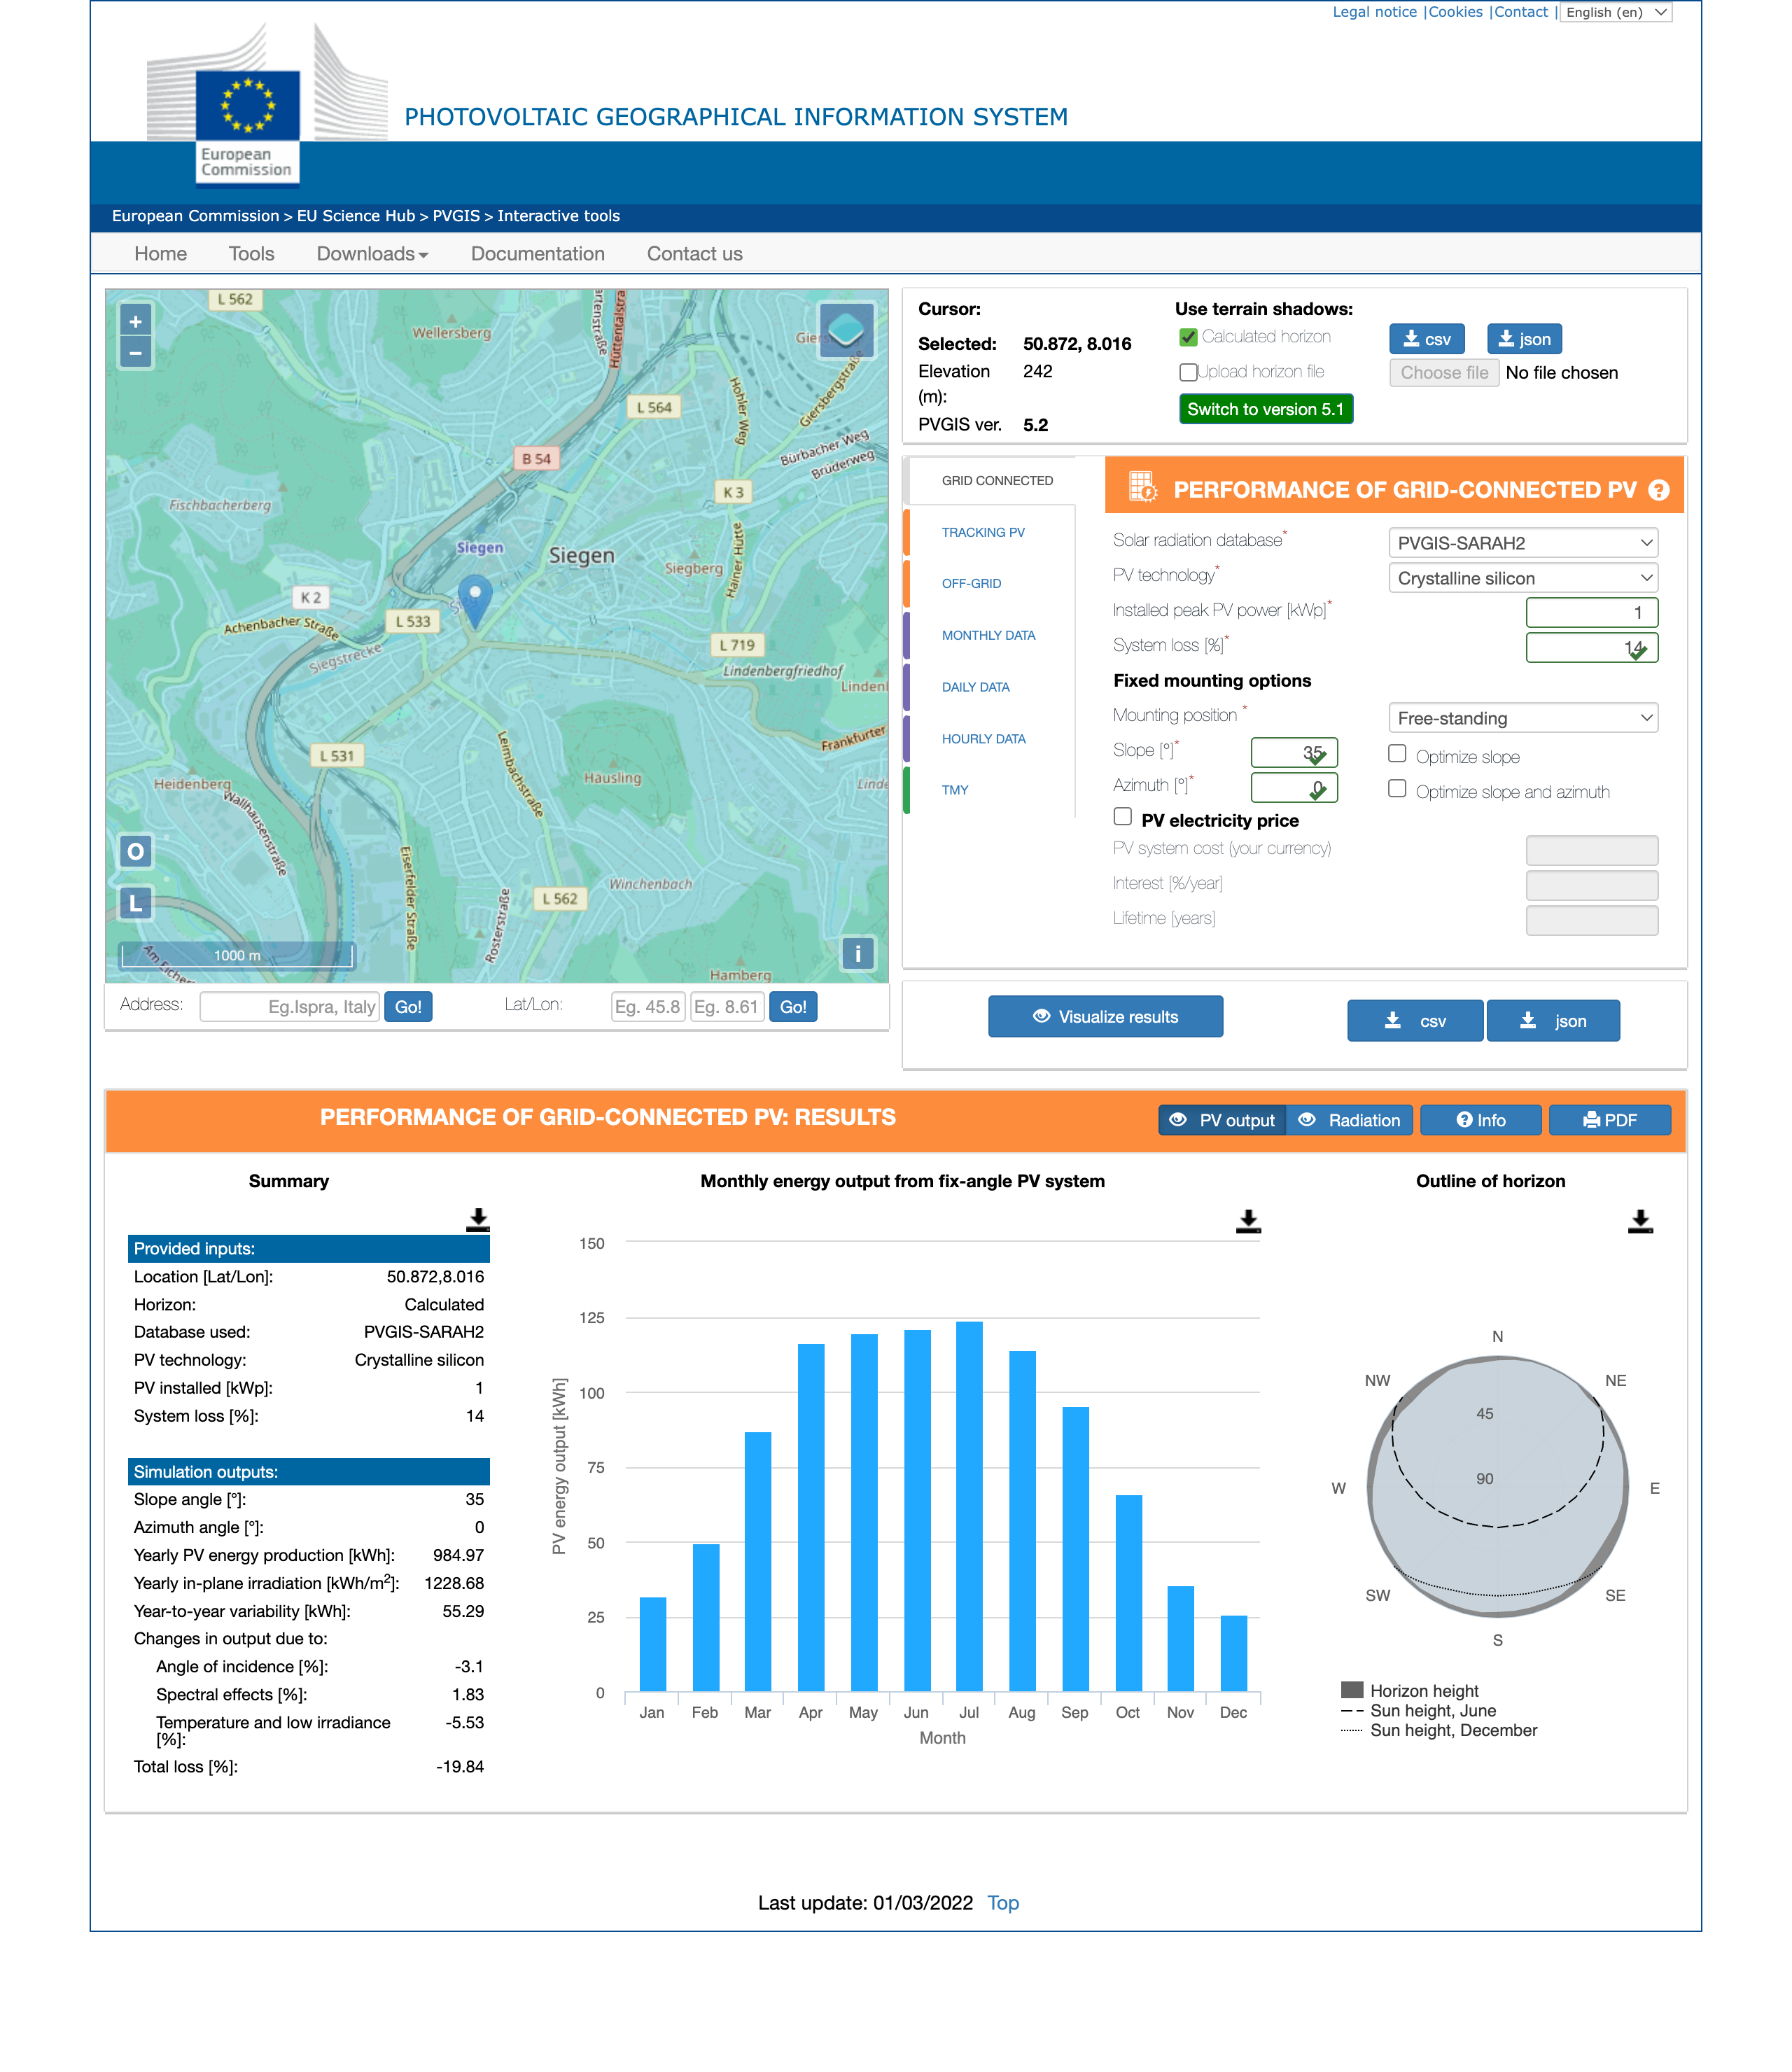
\includegraphics[width=\textwidth]{Images/pvgis.png}
  \caption{Screen of PVGIS online tool}
  \label{fig:pvgis}
\end{figure}


\subsection{FLEX models}

The FLEX models \cite{newtrends}, developed under the newTRENDs project\footnote{https://newtrends2020.eu/} by the Fraunhofer Institute for Systems and Innovation Research, 
aim to improve the building modeling suite and to analyse the societal trends of prosumaging and energy communities, 
are capable of calculating the energy demand of buildings at an hourly resolution,
while considering the impact of household behaviour, \gls{pv} generation, and energy storage (thermal and battery) on energy consumption. 
These models were developed to offer evidence-based information to decision-makers in industry, government, and civil society. 
%By providing a comprehensive assessment of the impacts of emerging technologies and innovation strategies, these models enable stakeholders to make informed decisions concerning policies related to technology and innovation. 

The models take various factors into account, including weather condition, household behaviours and energy technologies, as illustrated in Figure \ref{fig:flex-operation}.
Consequently, it offers a comprehensive evaluation of the energy consumption of a building. 
Moreover, the tool can be used to predict energy bills, enabling comparisons of energy expenses associated with different technology adoptions. 

%The Figure \ref{fig:flex} shows how FLEX interacts with other bottom-up models involved in the newTRENDs project,
%where FLEX-Operation and FLEX-Behaviour models are closely related to the demand and supply of energy for households. 
%\begin{figure}[h]
%  \centering
%  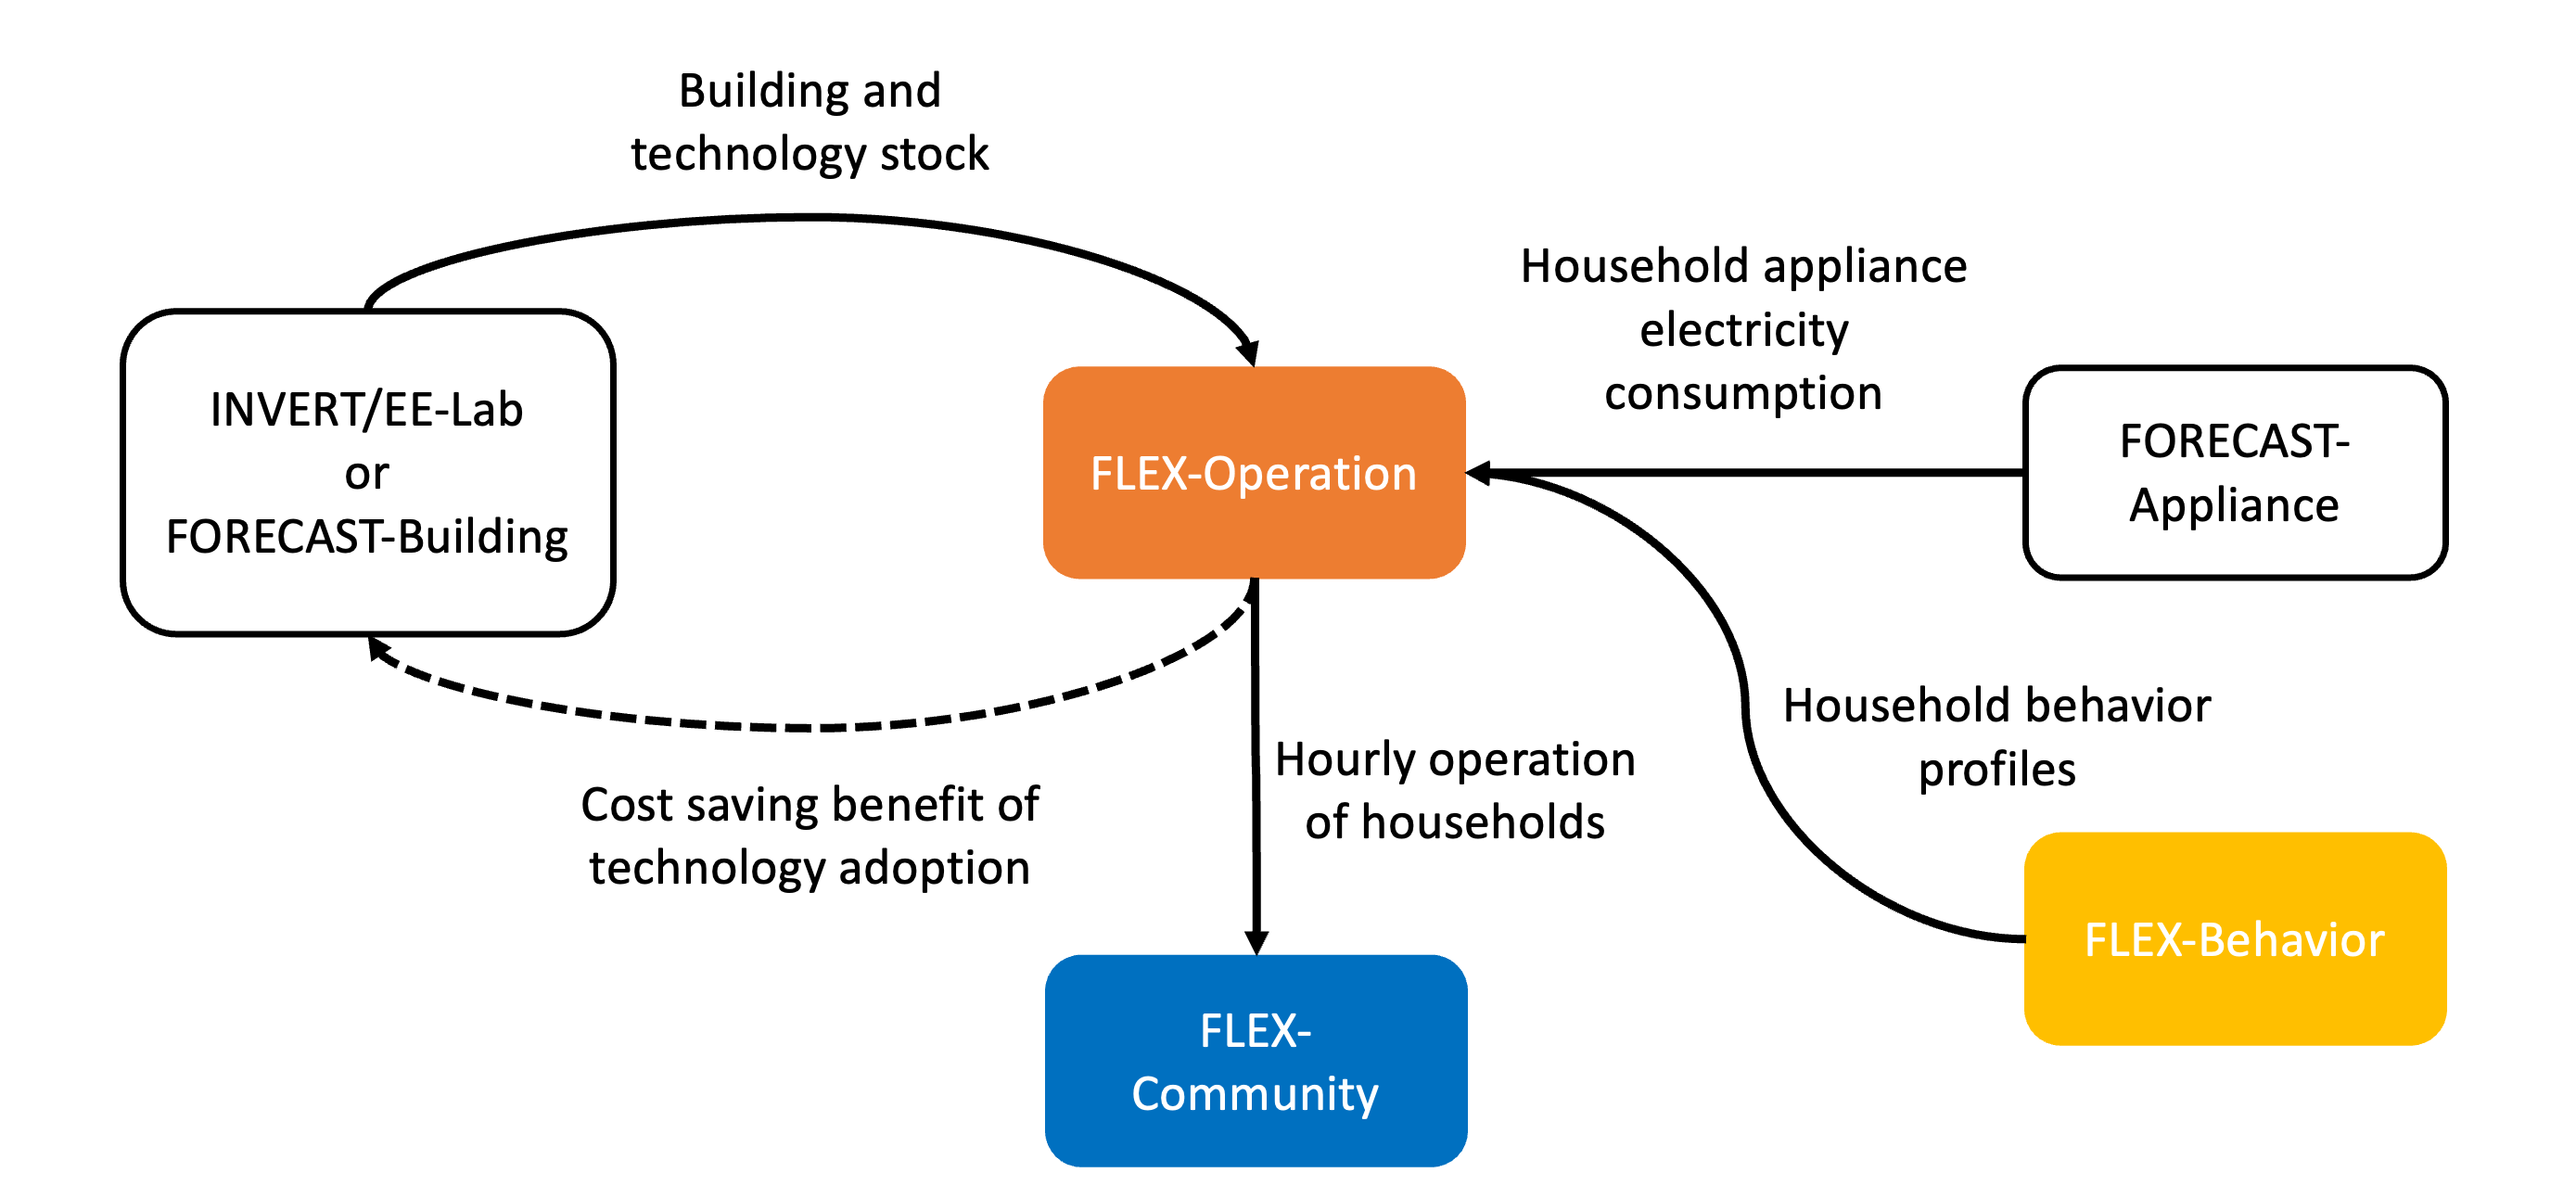
\includegraphics[width=\textwidth]{Images/flex.png}
%  \caption{FLEX modeling suite}
%  \label{fig:flex}
%\end{figure}

%Renewable energy (\gls{re}) and energy efficiency (\gls{ee}) are two central strategies pursued by the \gls{eu} and its Member States concerning the energy system. 
%In 2019, 80.9\% of our total energy supply still depended on burning fossil fuels, namely 26.8\% coal, 30.9\% oil and 23.2\% natural gas \cite{iea}. 
%Investments into low-carbon power generation accounted for 15\% recently are expected to rise to more than 30\% by 2030, corresponding to a quadrupling in absolute volumes \cite{shift}. Solar, wind, and the investments for enabling the integration of these technologies to the grid dominate the investments into low-carbon power generation \cite{shift}. 
%Electrification is playing a major role in the energy transition process. 
%Meanwhile, different electrification strategies rely heavily on energy efficiency \cite{electrification}.
%Measures to increase energy efficiency, including investments in energy savings and the consolidation of consultancy and information services, are promoted by The National Action Plan on Energy Efficiency (\gls{nape}) \cite{bafa}.  

%Transitioning towards a sustainable energy system necessitates significant effort on both the demand and supply sides. 
%However, previous research has shown that in many areas energy efficiency gains were counteracted by societal trends that increased corresponding activities, leading to much smaller decreases (or even increases) of energy demand than technologically feasible \cite{2050}. 
%The aim of newTRENDs is to increase the qualitative and quantitative understanding of impacts of new societal trends on energy consumption and to improve the modelling of energy demand, energy efficiency and policy instruments \cite{fraunhofer}. 


%\subsubsection{The FLEX-Operation model}

%The FLEX-Operation model \cite{newtrends} enables the detailed simulation of energy system operation for individual households at an hourly resolution. 
%This model provides a comprehensive assessment of the energy consumption of a representative building, incorporating technology operation (such as battery, \gls{pv}, and \gls{hp} systems) and load profiles at an hourly resolution. 
%In addition to its capability of modeling energy system operation, FLEX-Operation can also aid in investment decision-making by evaluating the energy-saving benefits associated with technology adoption.
%
%As shown in Figure \ref{fig:flex-operation}, FLEX-Operation considers following services:

%\begin{enumerate}
%  \item electric appliances, e.g., television, refrigerator, lighting, etc.;
%  \item space heating;
%  \item domestic hot water;
%  \item space cooling;
%  \item vehicle. 
%\end{enumerate}

\begin{figure}[h!]
  \centering
  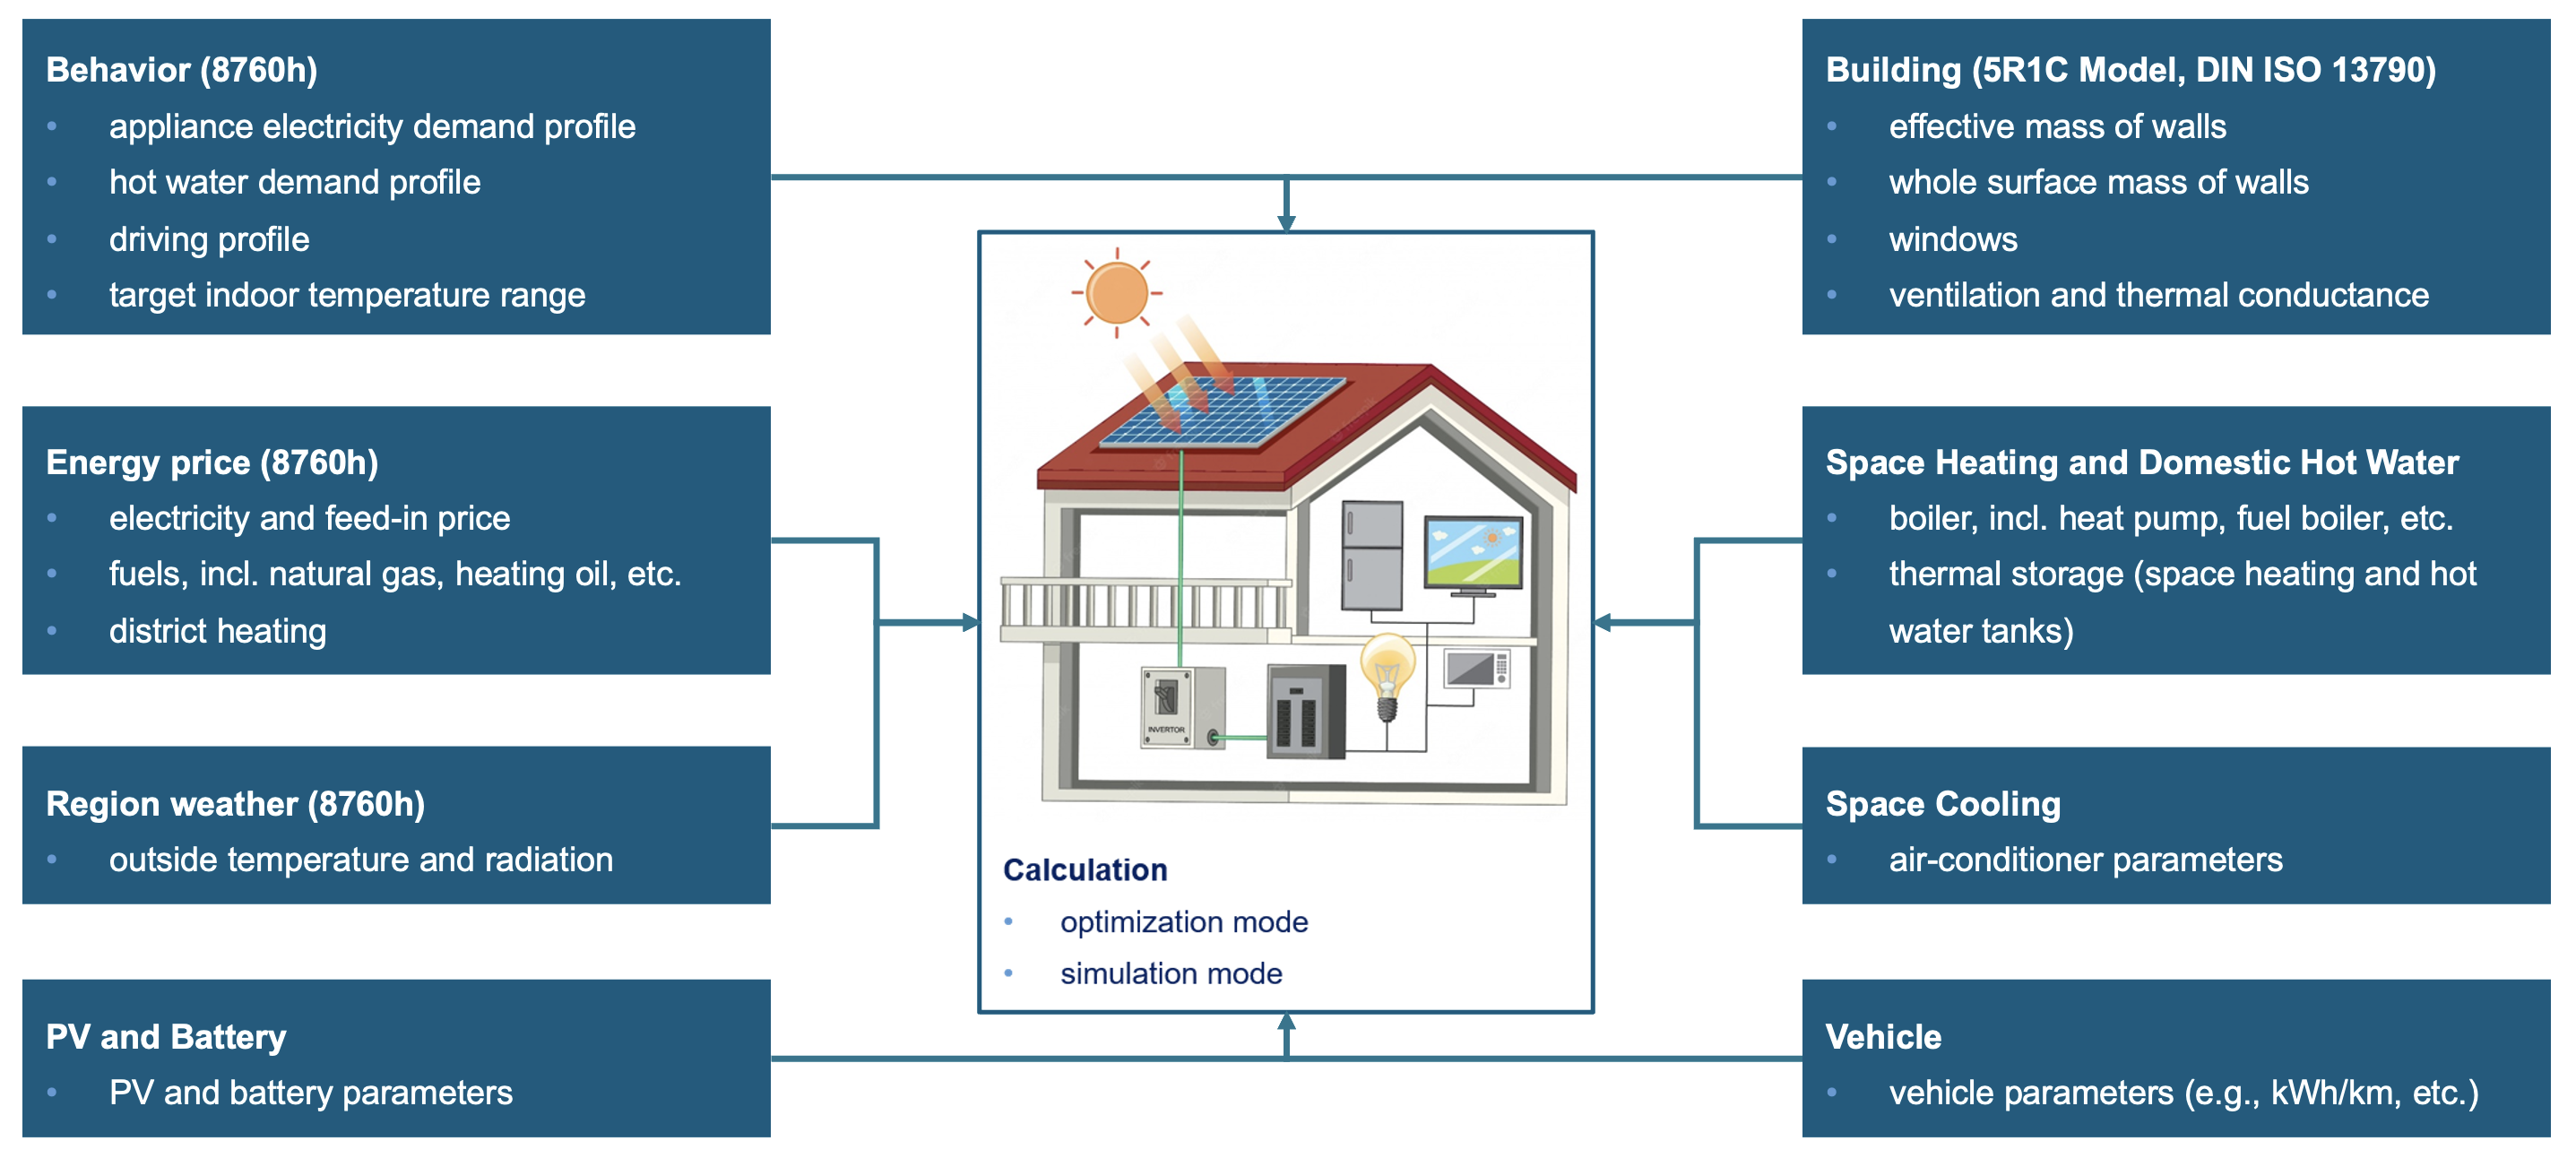
\includegraphics[width=\textwidth]{Images/flex-operation.png}
  \caption{Model structure for individual households}
  \label{fig:flex-operation}
\end{figure}

%Researchers believe new societal trends have the potential to shift energy demands between sectors and might reinforce or diminish one another when they occur at the same time \cite{2050}. 
%Researchers and organisations are paying increasing attention to how new societal trends are affecting energy demand.
%It is therefore important to access current and (foreseeable) future societal trends concerning the impact that they might have on future energy demand \cite{2050}. 

%Four arising societal trend clusters that are likely to shape future energy demand in European countries (and worldwide) were established by Brugger et al. \cite{2050}:  
%\emph{
%  (1) the digitalization of the economy and of private life; 
%  (2) new social and economic models, including the sharing economy and prosumaging (combination of producing, consuming and managing of energy); 
%  (3) industrial transformation, including decarbonization of industrial processes and the circular economy (including a stronger focus on material efficiency); 
%  (4) quality of life, including health effects, urbanization and regionalization. 
%}
%
%\begin{itemize}
%  \item \textbf{Digitalization of life} %\\ the digitalization of the economy and of private life;
%  \item \textbf{New social and economic models} %\\ including the sharing economy and prosumaging (combination of producing, consuming and managing of energy);
%  \item \textbf{Industrial transformation} %\\ including decarbonization of industrial processes and the circular economy (including a stronger focus on material efficiency);
%  \item \textbf{Quality of life} %\\ including health effects, urbanization and regionalization. 
%\end{itemize}
%
%The newTRENDs project develops the analytical basis for a “2050 Energy Efficiency Vision” by considering new societal trends in energy demand modeling \cite{newtrends}. 
%Considering the impact of these new societal trends on energy demand from a closer sectoral perspective,
%Yu et al. \cite{newtrends} identified four energy sectors: 
%
%\begin{itemize}
%  \item industry, 
%  \item transport,  
%  \item tertiary, 
%  \item residential.  
%\end{itemize}

%This proposed thesis will focus on the residential sector while taking scenarios of “consumers” becoming “prosumers” (with \gls{pv}) and “prosumagers” (adding energy storage and \gls{sems}) \cite{consumer} into account.  



%\subsubsection{The FLEX-Behaviour model}

%The FLEX-Behaviour model \cite{newtrends} facilitates the modeling of household behavior, including activity profiles and corresponding load profiles. 
%By generating an hourly activity and energy demand profile for a pre-defined household, this model provides a comprehensive assessment of the energy consumption patterns of an individual household.
%
%The estimates generated by the FLEX-Behaviour model refer to: 
%\begin{itemize}
%  \item appliance electricity demand,
%  \item domestic hot water demand,
%  \item driving profile, and
%  \item building occupation.
%\end{itemize}

%\subsubsection{INVERT/EE-Lab and FORECAST-Appliance}
%
%INVERT/EE-Lab and FORECAST-Appliance are the two models that can cover the energy consumption of residential buildings. The two models complement each other and cover the total energy consumption of households. 
%However, both INVERT/EE-Lab and FORECAST-Appliance calculate the energy consumption at the annual resolution and cannot model the prosumaging behavior and energy community, which requires an hourly resolution to consider the impact of household behavior, \gls{pv} generation, and energy storage (thermal and battery) on energy consumption. 
%In this regard, the FLEX-Operation and FLEX-Community models were developed to improve the building modeling suite and support relevant policy analysis \cite{newtrends}. 

%\subsubsection{FLEX-Community}
%
%FLEX-Community models the operation of an energy community, i.e., household interaction, aggregator optimisation. 
%It can be applied to support the aggregators designing and evaluating business models, as well as making investment decisions, for example, the self-owned battery, \gls{pv} panels, etc. \cite{newtrends}.


It is important to note that the FLEX models are designed to estimate for single building structures, meaning buildings that do not share walls with other buildings. 
Furthermore, the FLEX models are implemented in Python. 
To execute these models, users would need to have Python installed on their systems. 
Additionally, since the FLEX models involve complex optimisation problems, a solver is required. 
Users would need to download and set up the appropriate solver to run the FLEX models effectively.
Moreover, the outputs generated by the FLEX models are in the form of SQL files, 
which might not be immediately interpretable to non-technical users.


\section{Relevant theories}

The understanding of energy technologies and their implications in domestic settings can be regarded as a form of knowledge claims \cite{Bolisani2018}.
Given this, the process of obtaining this knowledge can be likened to a learning journey.
To enhance the dissemination of this knowledge to homeowners, learning theories are integrated into the design concept.


\subsection{Constructivism}

Constructivism, a psychological learning theory, delineates how individuals acquire knowledge and learn. 
It regards the learner as an active participant in knowledge assimilation.
This theory emphasises that individuals construct knowledge and meaning from their experiences. 
It advocates for an approach to teaching and learning where cognition (learning) is the result of "mental construction",
in essence, students learn by connecting new information to their existing knowledge \cite{Bada2015}. 

The integration of constructivist concepts aims to bridge the information gap by tailoring personalised recommendations to the unique contexts of individual households.
These theoretical frameworks propose that users are more inclined to grasp information about technologies and their advantages when they can relate the knowledge to their specific home energy systems.
By aligning information with their unique situations, users are more likely to engage and retain knowledge due to the contextual relevance of the recommendations.


\section{Transition to recommendation systems}

Recommender systems (\gls{rs}) are software tools and techniques designed to provide users with suggestions for items that might be of interest, 
assisting in various decision-making processes \cite{Ricci2011}. 
\gls{rs}s primarily target individuals who may lack the personal experience or expertise to evaluate an extensive range of alternatives \cite{Ricci2011}. 
In the context of homeowners seeking insights into energy technologies, 
\gls{rs} becomes particularly valuable, aiding those who are not well-versed in this domain to navigate the vast array of available options.

Building upon Constructivist theories of learning \cite{Bada2015}, 
this study emphasises a user-centric approach, aiming to bridge the information gap for homeowners.
Incorporating the learning theory, the focus is on linking new knowledge to existing experiences. 
Through \gls{rs} integration, users can merge the new knowledge of energy technologies with their present home energy systems, 
enabling a more comprehensive understanding and fostering a contextualised learning process.
Integrating \gls{rs} into the design concept aligns with the principles of Constructivism,
as it empowers users by enabling them to construct their understanding by associating new energy technology knowledge with their current home systems.

\gls{rs}s have a variety of properties that may affect user experience, 
such as accuracy, robustness, scalability, and so forth \cite{Shani2011}. 
However, in this study, our primary focus lies on the aspect of trustworthiness, 
recognised as an important consideration in \gls{rs} design \cite{Donovan2005}.

Drawing from Kirsten Swearingen and Rashmi Sinha's research \cite{rs},
specific recommendations are suggested to cultivate trust within a recommendation system.
Their proposed measures aim to promote trust by:
\emph{
  ensuring transparent system logic; 
  suggesting novel items; 
  offering comprehensive information about recommended items; 
  and enabling users to refine their recommendations by specifying preferred or excluded genres.
}

In summary, the integration of \gls{rs} within the design concept stands as an attempt to bridge the information gap 
by combining theoretical learning frameworks with a personalised recommendation system. 
This aims to enhance user learning experiences and foster more informed decisions regarding sustainable energy technologies for households.


\section{Conclusion}

%financial aspects play a significant role in guiding homeowners' decisions when considering upgrades to their home energy systems. 
Our exploration of the current practices and potentials within the domain of energy technologies and homeowner accessibility to information has revealed a noticeable information gap. 
Homeowners face limitations in obtaining comprehensive insights into energy technologies and their potential benefits.
The current approach, energy audits, can be quite laborious, 
involving booking appointments with experts, conducting house inspections, and investing considerable time in the assessment process. 
While government financial support might make the audits affordable, 
the effort required can discourage homeowners from seeking information and exploring energy-efficient options for their homes.

On the other hand, research-based models, particularly the FLEX models, 
are powerful tools that offer valuable insights through their detailed data and precise estimations of energy consumption and associated energy bills. 
These models consider various factors, including the house's characteristics, location, and energy technologies configuration. 
However, running these models demands professional knowledge, making them less accessible to general homeowners.
This creates an opportunity for the development of an innovative IT artefact that could revolutionise the way homeowners access information about energy technologies. 

The foundational principles of constructivism demonstrate the importance of contextual relevance in understanding and retaining knowledge.
These theories underpin the approach of personalising recommendations to individual home situations.
This artefact aims to empower homeowners with easy access to information, enhancing their understanding and fostering informed decisions regarding sustainable energy technologies for their homes.
\chapter{Methodology} 

The study uses Design Case Studies \cite{dcs} as the research framework. 

In the pre-study phase, 
the primary focus was to investigate existing practices and tools that can aid homeowners in gaining knowledge about renewable energy and energy-efficient technologies, as well as their benefits. 
To achieve this, we conducted searches online and reviewed relevant literature to gather information. 
As there were limited successful initiatives available in the market, we identified two related options: energy audits and research models. 
We studied both options to identify effective methods that can support homeowners in understanding renewable energy and energy-efficient technologies, along with their associated benefits.

Following the pre-study, 
we recognised a suitable approach aligned with the learning theory, 
and developed an innovative design concept: a personalised home energy system recommender.
To ensure its effectiveness, 
we started by investigating homeowners' motivations for investing in energy technologies through literature. 
Next, our focus was on providing recommendations that are aligned with user needs, 
and we placed great emphasis on enhancing the explainability of the system.

Furthermore, during the IT artefact design process, 
multiple factors were taken into account, including usability, user experience, and the chosen medium. 
Additionally, 5 formative evaluations were conducted on high-fidelity wireframes, 
which helped identify some issues that were then addressed through design iterations. 

After the service was programmed and made available online, 
we conducted a summative investigation to assess the appropriation of the artefact,
with a specific focus on two aspects:
\begin{enumerate}
    \item Do users enhance their knowledge about energy technologies and the advantages of their adoption through the service?
    \item Do users have trust in the recommendations provided by the system?
\end{enumerate}
6 qualitative evaluations were performed with 7 actual house owners. 
These evaluations were conducted through semi-structured interviews, 
each lasting approximately one to three hours. 

After conducting the evaluations, a thematic analysis was performed to gain deeper insights into users' experiences and perceptions. 
This analysis provided valuable feedback and insights that can be used for the next design iteration, allowing for further improvements and enhancements to the artefact. 

%The methodology adopted in this study is based on the Design Case Studies framework. 
%The pre-study phase will begin by conducting a comprehensive review of the literature to identify best practices for providing households with personalised and professional home energy system recommendations, as well as techno-economic assessments.
%Based on the findings from the pre-study, I will then design the interfaces of the intervention. 
%The interfaces will be developed to provide an intuitive and user-friendly experience that can easily be understood by households. 
%Following the development phase, real users will be invited to use the intervention, and feedback will be collected both qualitatively and quantitatively. 
%The qualitative data will be collected through interviews with participants, while the quantitative data will be collected through surveys. 
%Finally, the collected data will be analysed to evaluate households thoughts about the recommendations and energy technologies. 
%The entire process will be documented and reported in the form of a thesis. 
\chapter{Design} 

In order to bridge the information gap regarding home energy systems, this study aims to provide households with knowledge of available technologies in the market. 
To address the potential issue of information overload, the study proposes a home energy system recommender to present households with a tailored selection of technologies that better fit their unique home situations, 
such as by learning the location of the house, in order to estimate the amount of sunlight it is likely to receive over the course of a year, to evaluate whether installing a \gls{pv} system would be a viable and effective way for the household.
The learning theory suggests that individuals learn new knowledge by connecting it with existing knowledge and experiences, as this helps to create a framework for understanding and retention of the new information.
Therefore, by focusing on personalised recommendations, the study hypothesises that households may be more receptive to learning about home energy technologies. 
Additionally, with the intention of nudging house owners towards making informed decisions. 

\section{Design concept}
The design concept of the home energy system recommender involves the utilisation of personalised recommendations based on the unique situations of households. 
By gaining a deep understanding of the household's energy demands and supply dynamics, the recommender can offer tailored recommendations to optimise energy efficiency and costs. 
Through this approach, the recommender not only provides guidance on these technologies but also educates the house owners on the potential benefits of transitioning to more sustainable energy sources. 
To ensure the effectiveness of the recommendations, clear and concise explanations are provided to enable users to make informed decisions.


\section{Input to the system}


\subsection{Household profiles}

The concept of household profile has been developed to gain insights into the energy demand and supply dynamics of households. 
To ensure the accuracy of this profile, various factors that may impact the household's energy consumption must be taken into consideration, as shown in Figure \ref{fig:profile}, including 
\emph{
    the external environment, 
    building materials, 
    energy consumption behaviors, 
    and the current home energy system. 
}
By creating such a profile, a comprehensive understanding of the household's situation can be attained, enabling the offering of more tailored and effective recommendations.
\begin{figure}[h]
    \centering
    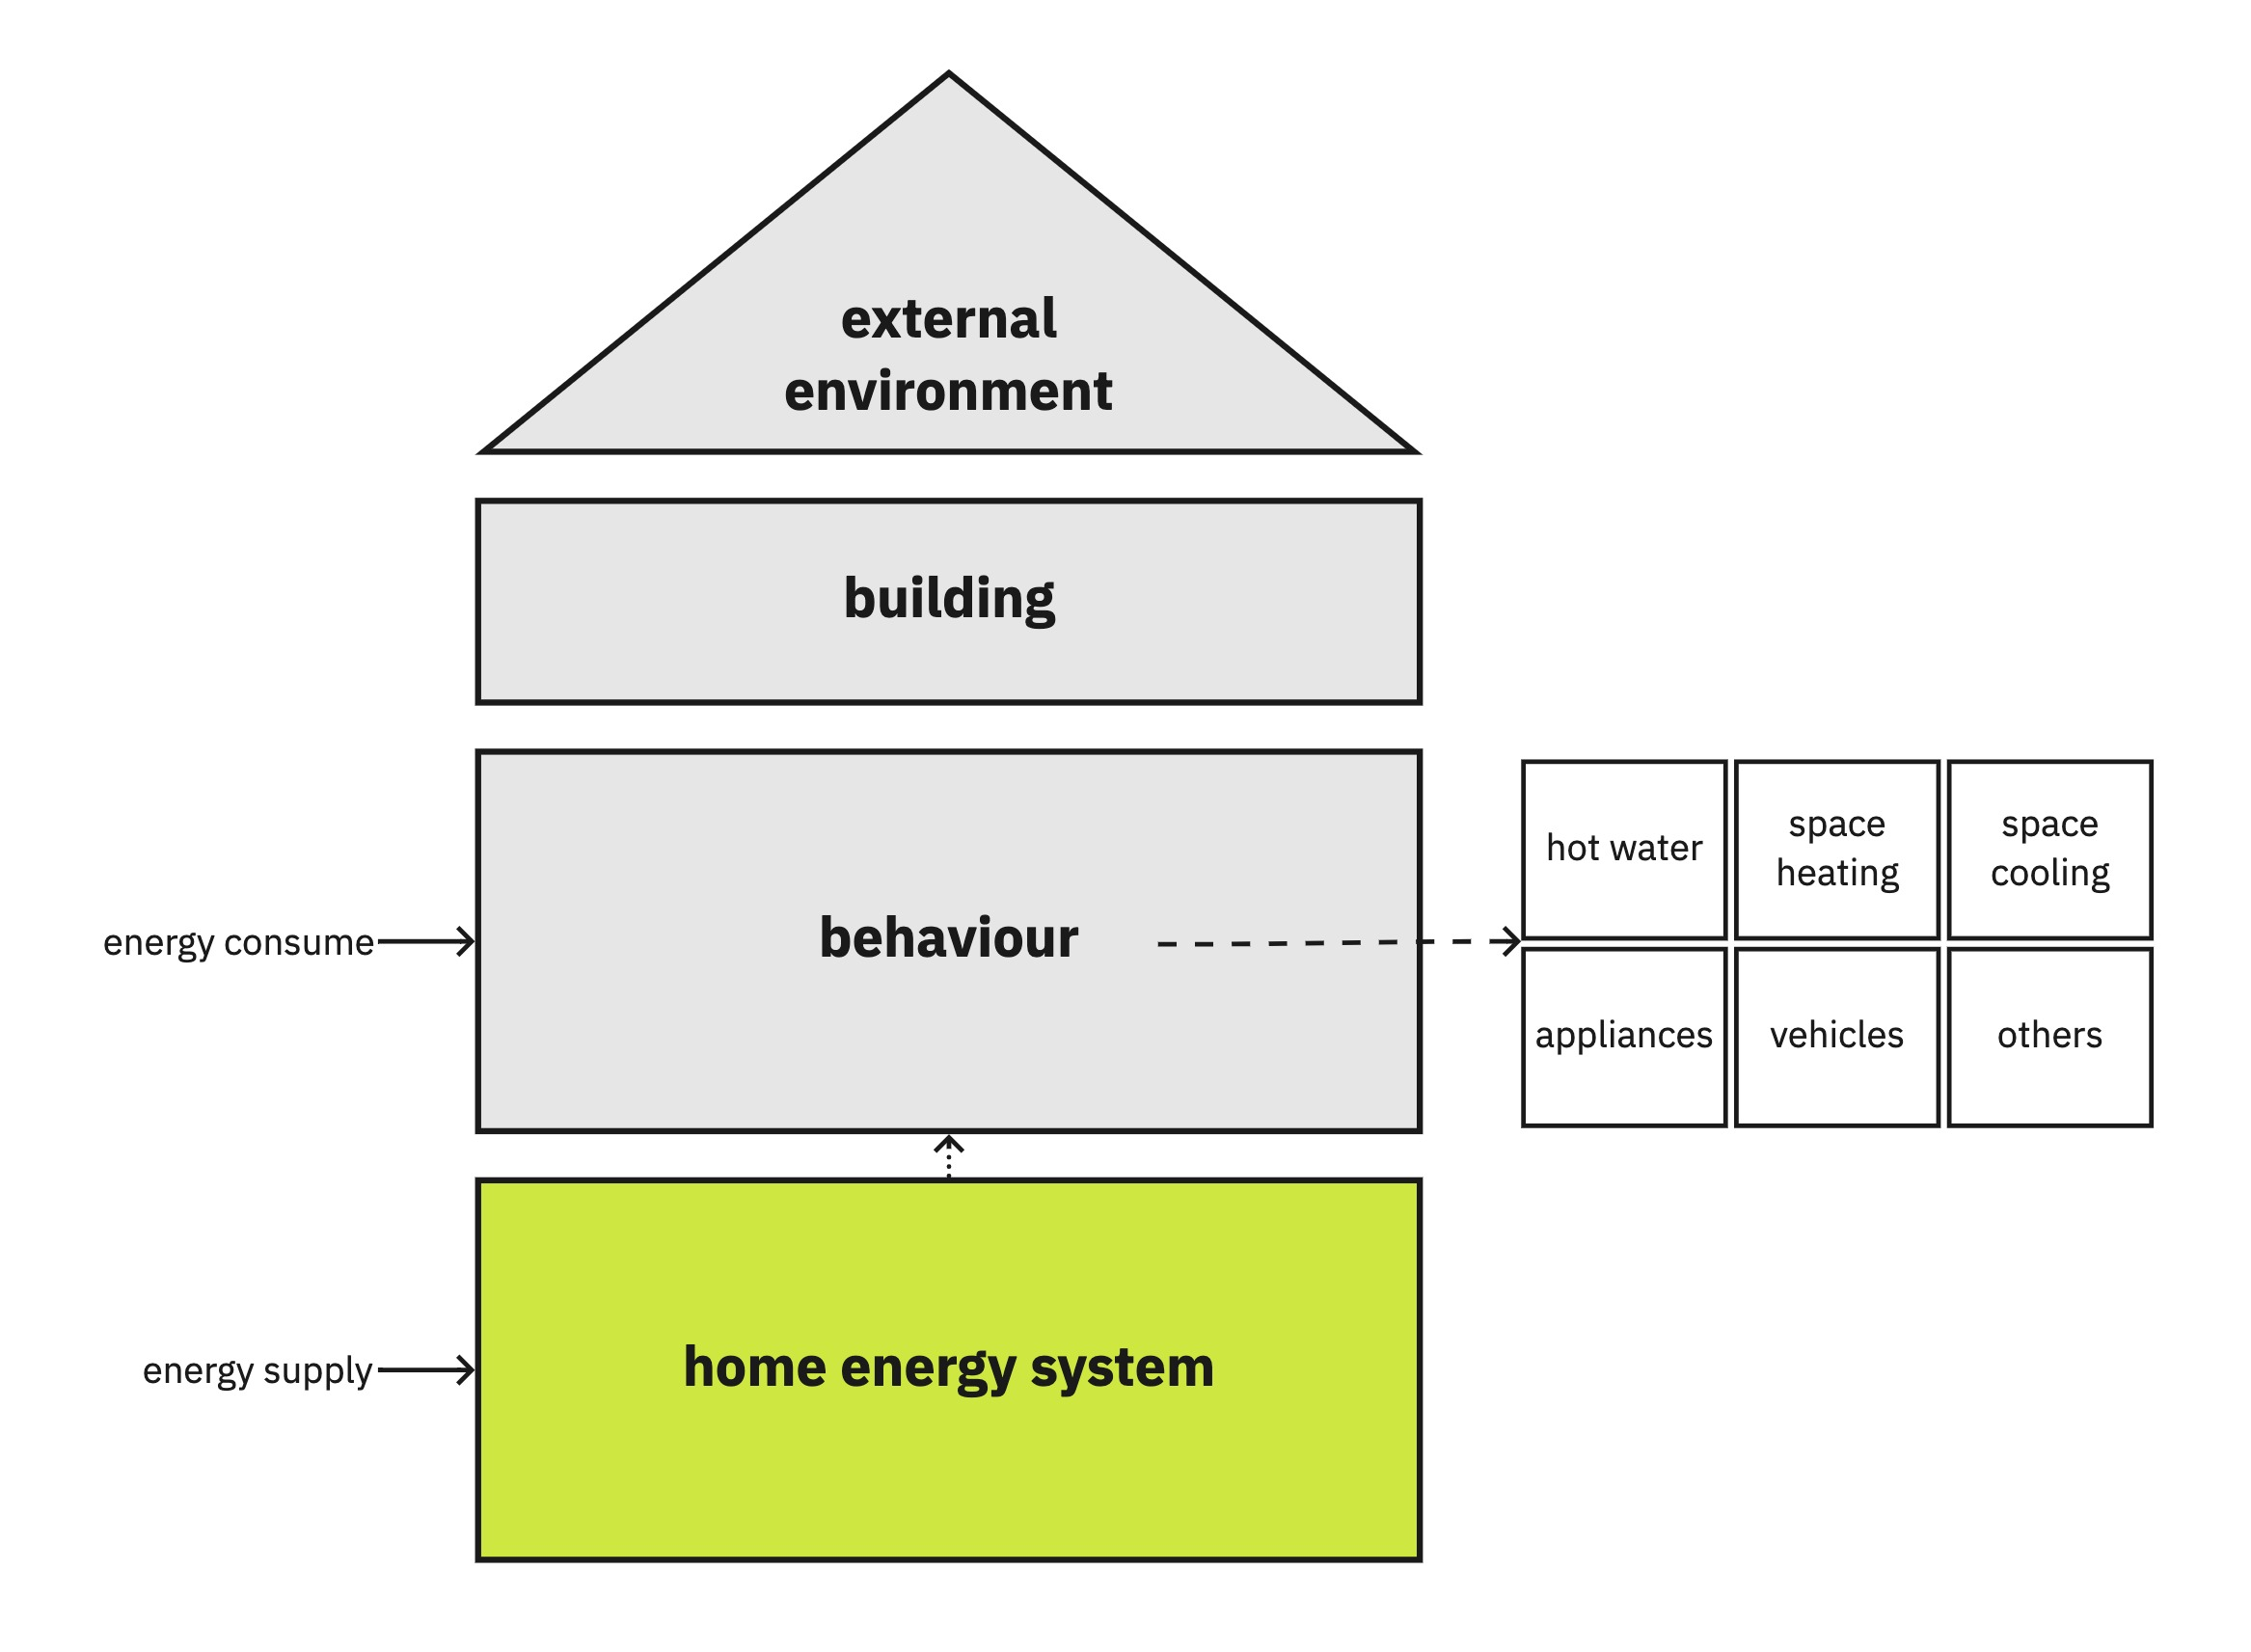
\includegraphics[width=\textwidth]{Images/household_profile.jpg}
    \caption{Household profile}
    \label{fig:profile}
  \end{figure}

\subsubsection{Input data by FLEX models}

In order to accurately anticipate household's energy costs,
the FLEX-Operation model takes a set of variables into account,
and they can be divided into following 15 categories: 
\emph{
    behaviour profile,
    battery,
    behaviour, 
    boiler,
    building,
    energy price,
    heating element, 
    hot water tank,
    \gls{pv},
    region,
    space cooling technology,
    space heating tank,
    vehicle,
    energy price,
    region weather. 
}
Furthermore, the specific data required by the FLEX-Operation model within each category can be found in Appendix \ref{appendix:inputdata}. 


\subsection{Decision trees for asking questions}

A total of 14 questions, see Table \ref{tab:questions}, were raised to collect all the relevant information necessary for the household profile analysis. 
In order to optimise the user experience, a decision tree approach was employed, allowing users to navigate through the questionnaire without the need to answer all the questions. 

\begin{center}
    \small
    \begin{longtable}{ | p{.15\textwidth} | p{.35\textwidth} | p{.35\textwidth} | }
        \hline
        Category & Question & Note \\
        \hline
        External environment & Where is the house located? & Understanding the location of the house can provide valuable insight into its environmental factors, such as the amount of sunlight it receives. \\
        \hline
        House condition & When was the house built? & Knowing the year a house was built can provide insight into its construction materials, such as the composition of the walls. \\
          & Has the house ever been renovated before? & Renovations can include upgrading insulation, replacing windows with energy-efficient ones, installing high-efficiency HVAC systems, sealing air leaks, etc. \\
          & What have been renovated in the house? &   \\
        \hline
        Energy use & How many people are living in the house? &   \\
          & How often does each adult work from home? &   \\
          & Is there any air conditioner in the house? &   \\
          & What type of heating energy is used in the house? &   \\
        \hline
        Home energy system  & Is there a photovoltaic (PV) system in the House? & A PV system is a system that uses solar panels to convert sunlight into electricity for use in a building. \\    
          & What is the size of the \gls{pv} system? &  The average size of a \gls{pv} system is 5 kilowatt-peak. \\
          & Is there a battery system in the house? & A home battery system is a device that stores energy produced by solar panels or other sources to be used later when needed. \\
          & What is the capacity of the battery? & The average capacity of a home battery system is around 7 kilowatt-hours. \\
          & Is there a smart energy management system in the house? &   \\
        \hline
    \caption{Survey questions}
    \label{tab:questions}
    \end{longtable}
\end{center}



\section{Output to the system}

\subsection{Recommendations}

An effective home energy system should prioritize minimizing energy waste, reducing dependence on non-renewable fossil fuels, and lowering overall energy costs. Our recommendations are aligned with these fundamental principles and aim to promote sustainable energy practices while also reducing household energy expenditures. 

The objectives of the recommendation system are multi-fold. 
Firstly, the system aims to support homeowners in making informed decisions regarding investments in home energy systems. 
Additionally, the system intends to encourage behavior change among homeowners by promoting the utilization of renewable energy sources. 
Finally, the recommendation system seeks to continuously refine and improve the accuracy of its predictive model, ensuring that the recommendations provided are up-to-date and effective. 
By providing users with tailored recommendations, the system aims to facilitate the adoption of energy technologies, ultimately leading to reduced energy demand and associated costs. 

As noted by Karen Palmer et al. \cite{informationgap}, financial considerations are of primary importance to homeowners when making decisions about energy investments. 
In line with this understanding, the recommendation system places a strong emphasis on providing transparent cost estimates for energy bills as well as recommended home energy system configurations. 
Additionally, the system seeks to encourage behavior change by providing information and education on climate change and renewable energy sources, aimed at increasing user awareness and understanding of the benefits of sustainable energy practices. 
To facilitate ongoing improvement and refinement of the recommendation system, a feedback survey button will be incorporated, allowing users to provide both short-term and long-term feedback on the system's performance and recommendations. 

\subsection{Explainability}

In order to provide more comprehensive and understandable recommendations, we have chosen to explain our recommendations from multiple perspectives beyond just cost estimates. 
Specifically, we have identified 4 key objectives, including \emph{trust, effectiveness, education, and debugging}, as key aspects to incorporate into our explanations. 
\emph{Trust}, we build trust with our users by using reliable data sources and providing transparent services. 
\emph{Effectiveness}, we strive to enhance the effectiveness of our service by offering recommendations that could actually benefit users economically. 
\emph{Education}, we seek to educate our users on the importance of environmental protection by sharing relevant knowledge and insights. 
\emph{De-bugging}, we value user feedback as an important tool for identifying and resolving any issues or bugs in our system, allowing us to continuously improve and refine our service.
The reasons for offering such explanations are to familiarise users with these technologies, establish accountability in the decision-making process, and encourage a shift towards environmentally conscious behaviour.
By incorporating these concepts into our explanations, we aim to provide recommendations that are transparent, trustworthy, understandable, and user-centred. 

Our recommendation system employs a three-level explainability framework to enhance user understanding of the recommended home energy system configurations. 
At the first level, the system provides an explanation in terms of the expected energy bill for the household. 
At the second level, the system offers a behavioural explanation of energy consumption patterns and the factors driving them. 
Finally, at the third level, the system aims to increase users' awareness and understanding of renewable energy and environmental protection.

Furthermore, the explanation is divided into three layers. 
At the first layer, users are provided with a comprehensive summary of their current energy consumption patterns. 
At the second layer, users are introduced to the various functionalities and benefits of the recommended energy technologies, including cost-saving potential and environmental impact. 
Finally, at the last layer, users are presented with simulated energy demand and supply data, allowing them to see the potential energy savings that could result from adopting the recommended configurations. 

Through the implementation of a comprehensive approach to explainability, our objective is to offer users an overview of energy technologies, enabling them to gain insight into their energy consumption patterns and to recognize the advantages of shifting towards more sustainable energy systems.


\subsection{Investments}

\begin{center}
    \begin{table}[h]
    \small
        \begin{tabular}{ | p{.30\textwidth} | p{.15\textwidth}  p{.15\textwidth}  p{.15\textwidth}  p{.15\textwidth} | }
            \hline
            Technology & \multicolumn{4}{ c | }{Cost (\euro{})} \\
             & Lowest & Highest & Installation & Maintenance \\
            \hline
            \gls{pv} system & \SI[per-mode=symbol,bracket-unit-denominator = false]{1957,68}{\per\kW}p & \SI[per-mode=symbol,bracket-unit-denominator = false]{2231,76}{\per\kW}p & included & 0 \\
            Battery system & \SI[per-mode=symbol,sticky-per,bracket-unit-denominator = false]{790,80}{\per\kWh}  & \SI[per-mode=symbol,sticky-per,bracket-unit-denominator = false]{2520,00}{\per\kWh} & included & 0 \\
            \gls{sems} & / & 1516,11 & 379,03 & 0 \\
            \gls{hp}& \SI[per-mode=symbol,bracket-unit-denominator = false]{432,15}{\per\kW} & \SI[per-mode=symbol,bracket-unit-denominator = false]{2370,31}{\per\kW} & included & 0 \\
            Hot water tank & 1 & 1 & 1 & 0 \\
            Space heating tank & 1 & 1 & 1 & 0 \\
            Air conditioner & 1 & 1 & 1 & 0 \\
            Basement renovation & \SI[per-mode=symbol]{132,12}{\per\metre\squared} & \SI[per-mode=symbol]{157,64}{\per\metre\squared} & included & 0 \\
            Roof renovation & \SI[per-mode=symbol]{40,95}{\per\metre\squared} & \SI[per-mode=symbol]{409,38}{\per\metre\squared} & included & 0 \\
            Wall renovation & \SI[per-mode=symbol]{67,57}{\per\metre\squared} & \SI[per-mode=symbol]{408,93}{\per\metre\squared} & included & 0 \\
            Window renovation & \SI[per-mode=symbol]{364,63}{\per\metre\squared} & \SI[per-mode=symbol]{958,92}{\per\metre\squared} & included & 0 \\
            \hline
        \end{tabular}
    \caption{Investment costs of different technologies}
    \label{tab:investments}
    \end{table}
\end{center}


\section{Interactions}

\subsection{Interfaces}

To facilitate user understanding of the recommended home energy system configurations and associated costs, our recommendation system will employ a visual and natural language explanation interface. 
Specifically, an interactive visualization tool will be implemented to enable users to explore and compare different energy system configurations in terms of energy consumption patterns and costs. 
Additionally, natural language explanations will be provided to further enhance user understanding and engagement with the recommended configurations. 


\subsection{Data visualisation}



\chapter{Development} 

The web application is designed, 
with the frontend responsible for collecting user data and presenting recommendations and explanations, 
while the backend handles the database generated by the FLEX models. 


\section{Frontend}

The frontend of the web application is responsible for creating an engaging and user-friendly interface using HTML, CSS, and JavaScript. 
They were used to structure the content, define the visual styles, and add interactivity to the application.
HTML is used to create the structure of the webpages, CSS is employed to style the visual appearance of the application. 
JavaScript plays a crucial role in adding interactivity and dynamic functionality to the web application. 
Additionally, JavaScript is responsible for making asynchronous requests to the server, facilitating communication with the backend.
To ensure a responsive design, the web application utilises the Bootstrap framework. 
Although the service is not intended for mobile screens, a responsive user interface that adapts to various devices and screen sizes has been taken into account. 


\subsection{Questionnaire}

To incorporate questionnaires into the web application, we integrated SurveyJS, an open-source JavaScript form builder library \cite{surveyjs}. 
SurveyJS simplifies the process of creating and embedding surveys.
It supports logic and branching, allowing for dynamic survey behaviour based on user responses, 
that fulfils our need of presenting corresponding questions according to the answers, as decribed in the design section. 


\subsection{Charts}

For chart building, we initially opted for Google Charts, a charting library provided by Google \cite{googlecharts}. 
However, we encountered difficulties in building multiple columns using Google Charts. 
As a result, we switched to Highcharts \cite{highcharts}, another powerful charting library written in JavaScript. 


\section{Backend}

The backend of the web application utilises Flask, a Python-based web framework \cite{flask}, to serve as the intermediary between the frontend and the FLEX models. 
This choice was made based on the fact that the FLEX models are implemented in Python. 
Originally, our intention was to enable direct communication between the backend and the models using Python. 
However, during the development process, we realised that the models' calculations, especially when finding recommended configurations, could be time-consuming. 
Each scenario takes approximately seven seconds to calculate, and considering the need to identify multiple scenarios that could save energy costs for the household, 
it would be impractical to make the user wait for the results. 
To address this issue, we decided to pre-process the data in the FLEX models and store it in a database. 
This approach significantly reduced the time required to identify energy-saving scenarios, allowing for a more efficient user experience.


\subsection{JSON Schema Documentation}

The API design for the service follows a RESTful architecture and adheres to the JSON schema presented in this section. 
This JSON schema defines the structure and properties of a household's energy system and recommendation.


\subsubsection{Household's energy system and recommendation}


\subsubsection{Properties}

The documentation consists of three main components: profile, current, and recommendation as displayed in table \ref{tab:properties}. 

\begin{table}[h!]
    \centering
    \small
    \begin{tabular}{ | p{.10\textwidth} | p{.10\textwidth} | p{.35\textwidth} | p{.10\textwidth} | p{.10\textwidth} | } 
      \hline
      Name & Type & Description & Required & Default value \\
      \hline
      profile & object & An object describing the house's location and number of people. & Yes & - \\
      \hline
      current & object & An object describing the house's current energy system configurations, energy data, and costs. & Yes & - \\
      \hline
      recom-men-dation & array & A list of recommended configurations that improve the house's energy efficiency. & Yes & - \\
      \hline
    \end{tabular}
    \caption{Properties}
    \label{tab:properties}
\end{table}


\subsubsection{Properties of profile}

As table \ref{tab:properties_profile} shows, the profile component provides information about the house's location and the number of people residing in it. 
It includes properties such as location and person.

\begin{table}[h!]
    \centering
    \small
    \begin{tabular}{ | p{.10\textwidth} | p{.10\textwidth} | p{.35\textwidth} | p{.10\textwidth} | p{.10\textwidth} | } 
    \hline
    Name & Type & Description & Required & Default value \\
    \hline
    location & string & The location of the house. & Yes & - \\
    \hline
    person & integer & The total number of people residing in the house. & Yes & - \\
    \hline
    \end{tabular}
    \caption{Properties of profile}
    \label{tab:properties_profile}
\end{table}


\subsubsection{Properties of current}

The current component describes the house's current energy system configurations, energy data, and costs. 
It consists of two properties: config and energy\_data. 
See table \ref{tab:properties_current}.

\begin{table}[h!]
    \centering
    \small
    \begin{tabular}{ | p{.10\textwidth} | p{.10\textwidth} | p{.35\textwidth} | p{.10\textwidth} | p{.10\textwidth} | } 
    \hline
    Name & Type & Description & Required & Default value \\
    \hline
    config & object & An object describing the house's current energy system configurations. & Yes & - \\
    \hline
    \makecell{energy\_\\data} & object & An object describing the energy demand, PV generation, and energy cost. & Yes & - \\
    \hline
    \end{tabular}
    \caption{Properties of current}
    \label{tab:properties_current}
\end{table}


\subsubsection{Properties of config}

The config property, as shown in table \ref{tab:properties_config}, captures the current energy system configurations, including parameters such as pv\_size, battery\_capacity, sems, heating\_system, heating\_system\_type, and building\_renovation.

\begin{table}[h!]
    \centering
    \small
    \begin{tabular}{ | p{.10\textwidth} | p{.10\textwidth} | p{.35\textwidth} | p{.10\textwidth} | p{.10\textwidth} | } 
    \hline
    Name & Type & Description & Required & Default value \\
    \hline
    pv\_size & integer & Determine the size of the PV system. & Yes & - \\
    \hline
    \makecell{battery\_\\capacity} & integer & Determine the capacity of the battery system. & Yes & - \\
    \hline
    sems & boolean & Determine the state of a SEMS system. & Yes & - \\
    \hline
    \makecell{heating\_\\system} & boolean & Determine the state of the heating system used.	 & Yes & - \\
    \hline
    \makecell{boiler\_\\type} & string & Determine the type of heating system used. & Yes & - \\
    \hline
    \makecell{building\_\\renovation} & boolean & Determine the state of the renovation. & Yes & - \\
    \hline
    \end{tabular}
    \caption{Properties of config}
    \label{tab:properties_config}
\end{table}


\subsubsection{Properties of energy\_data}

The energy\_data property contains data related to energy demand, PV generation, and energy cost. 
It includes properties like energy\_demand, energy\_generate, heating, cooling, appliance, hotwater, pv, and energy\_bill\_year.
See table \ref{tab:properties_energydata}. 

\begin{table}[h!]
    \centering
    \small
    \begin{tabular}{ | p{.10\textwidth} | p{.10\textwidth} | p{.35\textwidth} | p{.10\textwidth} | p{.10\textwidth} | } 
    \hline
    Name & Type & Description & Required & Properties in Database \\
    \hline
    \makecell{energy\_\\demand} & integer & The total energy demand in a year. & Yes & - \\
    \hline
    \makecell{energy\_\\generate} & integer & The total energy generated by PV in a year. & Yes & - \\
    \hline
    heating & array & The energy demanded for heating in the house for each month. & Yes & \makecell{E\_\\Heating\_\\HP\_out \\+ Q\_\\Heating\\Element} \\
    \hline
    cooling & array & The energy demanded for cooling in the house for each month. & Yes & \makecell{E\_\\Room\\Cooling} \\
    \hline
    appliance & array & The energy demanded by all appliances in the house for each month. & Yes & \makecell{BaseLoad\\Profile} \\
    \hline
    hotwater & array & The energy demanded for hot water in the house for each month. & Yes & \makecell{E\_DHW\_\\HP\_out} \\
    \hline
    pv & string & The energy generated from PV in the house for each month. & Yes & \makecell{Photo\\voltaic\\Profile} \\
    \hline
    \makecell{energy\_\\bill\_\\year} & integer & The total yearly energy cost. & Yes & - \\
    \hline
    \end{tabular}
    \caption{Properties of energy\_data}
    \label{tab:properties_energydata}
\end{table}


\subsubsection{Properties of recommendation}

The recommendation component represents a list of recommended configurations that can improve the house's energy efficiency. 
As listed in table \ref{tab:properties_recommendation}, each recommendation includes properties similar to the config and energy\_data properties in the current component. 
Additionally, it includes an investment\_cost property indicating the annualised investment cost for the recommended configuration. 

\begin{table}[h!]
    \centering
    \small
    \begin{tabular}{ | p{.10\textwidth} | p{.10\textwidth} | p{.35\textwidth} | p{.10\textwidth} | p{.10\textwidth} | } 
    \hline
    Name & Type & Description & Required & Default value \\
    \hline
    config & object & An object describing the recommended energy system configurations. & Yes & - \\
    \hline
    \makecell{energy\_\\data} & object & An object describing the energy demand, PV generation, and energy cost. & Yes & - \\
    \hline
    \makecell{investm\\ent\_cost} & integer & The annualised investment cost for the recommended configuration. & Yes & - \\
    \hline
    \end{tabular}
    \caption{Properties of recommendation}
    \label{tab:properties_recommendation}
\end{table}


\subsubsection{Example JSON data}

\begin{verbatim}
"energy_data": {
    "total_generate": <int>,
    "total_demand": <int>,
    "boiler": <int[12]>,
    "cooling": <int[12]>,
    "appliance": <int[12]>,
    "hotwater": <int[12]>,
    "pv": <int[12]>
},
\end{verbatim}

The JSON data example can be found in the appedix \ref{appendix:example_JSON}. 

\subsection{Endpoints}

The API exposes five endpoints to retrieve data,
they are survey\_scenario, scenario, recommendation, energy\_data, and eenergy\_cost.
The endpoints accept HTTP GET requests and returns JSON responses. 
\chapter{Evaluation}

In this chapter, we present the evaluation of our IT artefact. 
The evaluation study focuses on two main aspects. 
Firstly, we assess the effectiveness of the explanations provided to users in helping them understand why specific configurations were recommended for their home energy systems.
Secondly, we evaluate whether the information presented through the explanations has an impact on users' attitudes, such as increased awareness of energy-efficient technologies or a stronger inclination to adopt them. 
 
As highlighted in Nunes and Jannach's summary \cite{Nunes2020}, 
there is no universally accepted definition of what constitutes a correct or best explanation, 
evaluating the quality of explanations relies on capturing the subjective perceptions of users and monitoring the impact of these explanations on user behaviour, 
and user studies have been the predominant research method for assessing explanations in recommender systems.
Aligned with this understanding, our goal of capturing the subjective perceptions of users regarding the explanations provided and assessing any changes in their attitudes, 
we have made the decision to conduct real-user studies. 

Due to time constraints imposed by the university's requirements for a master's thesis, we conducted qualitative user studies with \textcolor{cyan}{6} participants in the \textcolor{cyan}{South Germany} region. 
While the sample size was small, qualitative studies provide valuable insights into rusers' perceptions, attitudes, and experiences.


\section{Semi-structured interviews}

The interview will follow the structured format to gather insights from the participants. 
\begin{enumerate}
  \item Express gratitude to the interviewee for their willingness to participate and introduce myself briefly.
  \item Provide a brief recap of the project, emphasising its purposes, and clarify the specific objectives of the interview.
  \item Inform the interviewee about the expected duration of the interview (approximately 40 minutes) and assure them that the recording will be used solely for transcription purposes, ensuring confidentiality.
  \item Explain that the interview will involve participants using the web service to explore and discover recommendations tailored to their home energy systems.
  \item Prior to participants using the service, they will be asked a series of questions pertaining to their demographic information and initial perceptions of energy technologies.
  \item Allow participants to utilise the service using a laptop.
  \item Once the participants have interacted with the service, other questions will be asked.
  \item Inquire if the interviewee has any remaining questions or uncertainties.
  \item Express appreciation once again for their participation and inform them that they can reach out with any further concerns or inquiries they may have.
\end{enumerate}


\subsubsection{Target groups}

The target users of this study are individuals residing in Germany who own single-family houses.
The participants were recruited using a convenient sampling approach. 
We employed a snowball technique by reaching out to acquaintances to inquire about their residence in a single-family house or their knowledge of individuals residing in such properties. 
Additionally, we extended our recruitment efforts to colleagues within Fraunhofer ISI.

The interview invitation is:

Are you a homeowner in Germany with a single-family house? 
Do you want to make informed investment decisions about energy technologies for your home? 
If so, we invite you to participate in a 40-minute interview for our web service developed in collaboration with the University of Siegen.
Don't miss out on the opportunity to test our web service, which provides personalised techno-economic investment recommendations tailored to your unique home situation. 
During the interview, you will use our online service and share your experience.
Rest assured that all information shared will be kept confidential and anonymised. 
The interview will be conducted remotely for your convenience.
If you are interested, please choose your preferred time slot by clicking on the following link: https://calendar.app.google/F8RnWSKmnofz3cHf6. 
If you have any questions, feel free to contact us.
Thank you for considering this exciting opportunity to collaborate on our project!

Every participant took part in the evaluation signed a consent form (Appendix \ref{appendix:consentform}) before starting. 

\begin{table}[h!]
  \centering
  \begin{tabular}{ | p{.10\textwidth} | p{.10\textwidth} | p{.10\textwidth} | p{.20\textwidth} | p{.20\textwidth} | } 
    \hline
    ID & Gender & Age & Nationality & Occupation \\
    \hline
    PA & M & 60 & Germany & Constructor \\
    \hline
    PB & M & 30 & Germany & Researcher \\
    \hline
    PC & F & 28 & Taiwan & HCI student \\
    \hline
  \end{tabular}
  \caption{Participants}
  \label{tab:participants}
\end{table}


\subsubsection{Goals}

\begin{itemize}
  \item Evaluate the effectiveness of explanations in helping users understand the rationale behind recommended configurations for their home energy systems.
  \item Assess the impact of the provided information on users' attitudes, including increased awareness of energy-efficient technologies and a higher propensity to adopt them. 
\end{itemize}


\subsubsection{Material}

\begin{itemize}
  \item \textbf{Laptop:} Participants will be provided with a laptop to access and use the web service before the interview. 
  \item \textbf{Recording Device:} A mobile phone for instance, will be used to capture and record the interview session to enable accurate transcription of the interview responses for analysis and reference.
  \item \textbf{Interview Guideline:} A printed copy of the interview guideline.
  \item \textbf{Pen and Papers:} A pen and some papers to jot down any notes or additional information during the session. 
  \item \textbf{Translator:} In the event that participants are not comfortable with the English language, a German speaker will be present to assist in facilitating communication and ensuring a clear understanding of the questions and responses.
\end{itemize}


\subsubsection{Welcome}

Thank you for participating in this interview. 
My name is Yanwei Miao, and I am currently working on my master's thesis project in collaboration with Fraunhofer ISI.
We developed a web service to help homeowners like you make informed decisions about investing in energy technologies for your homes. 
Our aim is to provide personalised recommendations based on your specific circumstances, enabling you to determine the economic feasibility of implementing these technologies. 
To proceed, we kindly request your cooperation in answering a few questions about your background. 
This will help us gain a better understanding of your knowledge and perspective on AI and energy. 
Once is complete, we will guide you through the web service to obtain personalised recommendations for your home energy system. 
While using the service, we encourage you to think out loud and share your thoughts and observations. 
Afterward, we will conduct a 30-minute interview to gather your feedback and insights. 
If you have any questions at any point, please don't hesitate to ask. 
Are you ready to begin?


\subsubsection{Questions}

The interview questions can be categorised into four main categories: \emph{demography, explainability, attitude change, and additional questions}.
Demography questions focus on gathering information about the background of the interviewees, aiming to identify any demographic factors that may influence their interest in more detailed explanations.
Explainability questions are designed to assess the clarity and comprehensibility of the provided explanations, aiming to determine if they are clear and understandable to the participants. 
Attitude change questions are divided into two parts: before using the service and after using the service. 
These questions aim to capture any changes in participants' attitudes towards energy technologies and their perception of the recommendations after using the service.
Lastly, additional questions or thoughts may arise during the interview. 
They could be an opportunity to explore additional insights or address any specific concerns during the conversation. 

\begin{center}
  \small
  \begin{longtable}{ | p{.20\textwidth} | p{.70\textwidth} | }
    \hline
    \textbf{Category} & \textbf{Questions} \\
    \hline
    \multicolumn{2}{|l|}{\cellcolor{lightgray}Before using the web service} \\
    \hline
    \multirow{6}{4em}{Demography} & Gender \\
    & Age \\
    & Educational background \\
    & Occupation \\
    & Knowledge and interest in AI \\
    & Knowledge and interest in the energy domain \\
    \hline
    \multirow{4}{4em}{Altitudes} & Have you heard of energy-efficient appliances or renewable energy technologies for households? \\
    & Have you ever considered implementing energy-efficient technologies, such as solar panels and smart thermostats in your house? \\
    & What is your understanding regarding the benefits of energy-efficient technologies? \\
    & Do you know climate change and why it is important for individuals to save energy and utilise renewable energy sources? \\
    \hline
    \multicolumn{2}{|l|}{\cellcolor{lightgray}After using the web service} \\
    \hline
    \multirow{4}{4em}{Altitudes} & How do you feel about the recommendations provided? \\
    & Do you find the recommendations useful or valuable? \\
    & Are you considering investing in any of the recommended technologies now? Why or why not? \\
    & What factors influence your decision to adopt or reject the recommendations? \\
    \hline
    \multirow{7}{4em}{Explainability} & Do you know why the recommendations were recommended to you? \\
    & Do you trust the recommendations? Why or why not? \\
    & What factors contribute to your trust or lack of trust in the recommendations? \\
    & Were you familiar with these technologies before using the system? \\
    & Did the system provide enough information for you to understand the technologies? \\
    & Has your knowledge of energy efficient technologies improved as a result of using the system? \\
    & Do you believe adopting these technologies can lead to lower energy costs? Why or why not? \\
    \hline
    \multirow{2}{4em}{Additionals} & Give participants an opportunity to share any additional thoughts, concerns, or suggestions regarding the system and its recommendations. \\
    & Ask if they have any questions for you or if there's anything else they would like to discuss. \\
    \hline
  \caption{Interview guideline}
  \label{tab:interview}
  \end{longtable}
\end{center}


\subsubsection{Closure}

Thank you so much for taking the time to participate in this interview session. 
I truly appreciate your willingness to share your thoughts and experiences with us. 
If you have any further questions, concerns, or additional insights that you would like to share, please don't hesitate to reach out.


\section{Future work: Kano survey}

The Kano model \cite{Sauerwein1996} is a commonly used framework in quantitative research to understand customer satisfaction and prioritise features or attributes. 
In our project, we aim to also incorporate the Kano model survey (Table \ref{tab:kanomodel}) as part of our future work. 
We plan to integrate this survey directly into the web service, allowing individuals who have interacted with the service online to voluntarily complete the survey.
Through the integration of the Kano survey into the web service, we have the opportunity to collect insights from users who engage with the service online. 
This will enable us to assess whether the inclusion of specific features in the service brings delight to our users.
This assessment will help us determine the necessity of explanations in the service. 

\begin{center}
  \small
  \begin{longtable}{ | p{.40\textwidth} | p{.06\textwidth} | p{.06\textwidth} | p{.06\textwidth} | p{.06\textwidth} | p{.06\textwidth} |}
    \hline
    Features & I like it & I expect it & I'm neutrual & I can tolerate it & I dislike it \\
    \hline
    Show corresponding yearly energy bill &&&&& \\
    \hline
    Don't show corresponding yearly energy bill &&&&& \\
    \hline
    Show detailed simulated yearly energy consumption &&&&& \\
    \hline
    Don't show detailed simulated yearly energy consumption &&&&& \\
    \hline
    Show detailed simulated daily energy consumption &&&&& \\
    \hline
    Don't show detailed simulated daily energy consumption &&&&& \\
    \hline
    Show climate change information &&&&& \\
    \hline
    Don't show climate change information &&&&& \\
    \hline
    Allow exploring and adjusting configurations of the recommended technologies &&&&& \\
    \hline
    Don't allow exploring and adjusting configurations of the recommended technologies &&&&& \\
    \hline
    Show comparison with current situation &&&&& \\
    \hline
    Don't show comparison with current situation &&&&& \\
    \hline
    Show explanation of each technology &&&&& \\
    \hline
    Don't show explanation of each technology &&&&& \\
    \hline
    Show total investment costs of each technology &&&&& \\
    \hline
    Don't show total investment costs of each technology &&&&& \\
    \hline
    Show annualised investment costs of each technology &&&&& \\
    \hline
    Don't show annualised investment costs of each technology &&&&& \\
    \hline
  \caption{Kano survey}
  \label{tab:kanomodel}
  \end{longtable}
\end{center}


\section{Analysis}

Table \ref{tab:participants_perceptions} summarises the participants' overall knowledge and interest in AI and energy, 
as well as their perspective on the altitude change and trust in the recommendations following their use of the service.  
In addition, all transcripts can be found in the appendix \ref{appendix:transcription}.

\begin{table}[h!]
  \centering
  \begin{tabular}{ | p{.10\textwidth} | p{.15\textwidth} | p{.15\textwidth} | p{.15\textwidth} | p{.15\textwidth} | } 
    \hline
    ID & Interest in AI & Interest in energy & Altitude change & Trust \\
    \hline
    PA & No & Yes & No & Yes \\
    \hline
    PB & No & Yes & No & Yes \\
    \hline
    PC & No & No & Yes & Not much \\
    \hline
  \end{tabular}
  \caption{Participants' perceptions about AI and energy}
  \label{tab:participants_perceptions}
\end{table}


\subsubsection{Participant A}

Before using the service, 
Participant A, who works in the house construction industry, 
displayed knowledge of EU energy policy and familiarity with energy-efficient appliances and renewable energy technologies. 
He had implemented solar panels in one of his houses and believed in their ability to reduce energy costs for households. 
Participant A emphasised the rising energy prices and the importance of addressing climate change, expressing dissatisfaction with Germany's continued use of coal. 

During the service usage, 
Participant A found the service to work smoothly, receiving a comprehensive list of around 50 recommendations to lower energy costs. 
While he agreed with most configurations, he felt overwhelmed by the extensive list and preferred to focus on specific options such as installing a heat pump and conducting a house renovation, given his expertise in his own house's needs. 
Despite not finding recommendations for biomass utilisation, Participant 1 relied on his professional experience and personal resources in considering biomass as the most cost-effective option. 
Although he missed the last level of explanation on renewable energy benefits, he clicked to view more details on the specific recommendation he sought.

After using the service, 
Participant A appreciated the recommendations but felt they were more suited for general houses rather than his unique situation. 
Financial considerations and environmental impact guided his energy technology decisions. 
Trusting the recommendations due to his familiarity with them, he acknowledged the service provided an overwhelming amount of information and a surplus of recommendations.


\subsubsection{Participant B}

Before using the service, 
Participant B, who works in the renewable energy industry, 
expressed a strong awareness of climate change and a desire to implement energy-efficient technologies and measures in his house primarily for economic reasons.

During the service usage, 
Participant B found the service to be simple, clean, and straightforward, which he appreciated. 
Although the service did not consider his electric car, he believed the estimation of the remaining energy bill to be accurate. 
He found the information on investment costs to be useful and liked the ability to adjust settings to see changes in energy demand and bill. 
While he noticed the "why turn to renewable energy" card, he did not click to view it.

After using the service, 
Participant B found it particularly helpful in determining the appropriate sizes for investment consideration. 
He believed that implementing these technologies could lead to energy cost savings, 
but expressed concern about the upfront investment amount, which posed a barrier for him. 
He suggested that government assistance in the form of support for monthly payments or other financial incentives could make green living more accessible. 
Participant B also suggested that the service should offer more comprehensive guidance on getting started 
and allow for more detailed inputs, such as providing options to enter specific details like roof size and receive insulation recommendations. 
He expressed trust in the recommendations, as the energy bill was accurate when not considering the electric car. 
The well-programmed and responsive website service contributed to his trust as well, and he appreciated that the interface was not overly complicated.


\subsubsection{Participant C}

Before using the service, 
Participant C, a current master's student in human-computer interaction, 
admitted that she doesn't have much knowledge or interest in artificial intelligence, energy, or energy technologies. 
She does have a smart thermostat installed on her heater, which was provided by her landlord, and she is familiar with how it operates. 
Additionally, her colleagues at work have also shared their experiences with smart thermostats, as many of them have one. 
She holds the belief that the concept of ,,energy efficiency" does not necessarily mean conserving energy but rather generating energy more efficiently, while ensuring human comfort.

During the service usage, 
Participant C carefully read all the explanation texts for each technology while providing the current configuration of her house. 
She wanted to ensure that she answered correctly. 
When selecting the battery capacity, she wasn't entirely sure about the size of the battery in her house, but with only two options available, she quickly made her choice, believing that the battery in her house should be a larger one.
After receiving the estimates of her current annual energy bill, Participant C calculated the monthly bill herself and was pleasantly surprised to find that it was very precise. 
She then proceeded to choose a recommendation and closely examined the accompanying energy graphs. 
Noticing that the energy demand bars for each month showed variations, with less demand in the summer and more in the winter, she found this pattern to be logical and sensible.
However, she also encountered a confusing aspect when she noticed an energy bar for cooling, even though she didn't have an air conditioner in her house. This information puzzled her. 
Participant C also clicked on the climate change education card to quickly scan its content and appreciated the information being presented in that section.

After using the service, 
Participant C found it to be a potential replacement for the Energieausweis, a nation-wide recognised standard in Germany for displaying a house's energy-efficiency level, which people usually need to pay professionals for. 
She appreciated that the recommendations were presented in a neutral manner, 
but suggested that more eye-catching visuals could make her feel the significant impact of potential savings and encourage her to make changes.

Participant C felt that the recommendations might not perfectly align with her own situation,
because the questions asked in terms of her energy consumption behaviours, were relatively general. 
She believed that more detailed and private questions could lead to a more personalised calculation. 
Regarding trust, she initially believed in the service, 
especially after seeing that the estimated energy bill was accurate. 
However, when she encountered confusion in the graph, her trust in the system wavered. 
Participant C had concerns that the service might be promoted by business companies with the intention to sell their products. 
This led her to believe that the algorithm behind the model might be biased and pushing users to spend money. 
However, after it was clarified that the project was solely a research-driven initiative sponsored by the EU without any commercial influence, she gained more trust in the service.
To further validate her trust in the system, she decided to test it by inputting the best energy configuration. 
The service did not provide any recommendation for this situation, which reinforced her belief that the system was not solely focused on pushing users to spend money. 
This positive experience increased her trust in the service and the recommendations. 

Participant C also mentioned that her investment willingness was influenced by various factors, 
including how long she planned to stay in her current house and whether she could take the technologies with her when moving. 
In her background, households were not allowed to privately install \gls{pv} systems without obtaining a certificate from authorities, 
and selling excess electricity back to the grid was prohibited. 
which differs from Europe where governments encourage \gls{pv} installations. 
Upon learning about these differences, she became enthusiastic about installing a PV system, 
recognising its benefits in both cost savings and contributing to environmental preservation.

Despite not having much prior knowledge of energy technologies, 
Participant C was able to answer all questions about her current house after reading the descriptions provided. 
She mentioned that the service allowed her to gain a rough understanding of these technologies but expected to learn more detailed benefits and information through the platform.
\chapter{Conclusion}

Our exploration to bridge the gap in knowledge about energy technologies and the associated benefits for homeowners has yielded valuable insights. 
The journey began with an initial phase of pre-study, where our goal was to uncover existing tools and practices that could empower homeowners to embrace sustainable energy solutions. 
This initial investigation paved the way for the development of an innovative home energy system recommender, anchored in the FLEX models. 
These models assist in identifying technology configurations tailored to specific situations, leading to potential energy cost savings that directly benefit homeowners financially. 
Throughout the development process, we placed significant emphasis on explainability, ensuring the recommendations were trusted.  
By engaging with real participants through user testing, we have gained a deeper understanding of their expectations, concerns, and attitudes. 
The insights gathered from the feedback lead us to a conclusive observation.


\section{Filling the information gap}

The provision of such information has a significant impact on the decision-making process of homeowners, even though there are slight variations in how different users respond. 
These differences are indicative of varying perspectives of positive attitudes towards investing in such technologies. 
For instance, users who had limited knowledge about energy technologies before using the service expressed that they gained a better understanding of various technologies, their functionalities, and the potential financial benefits.
On the other hand, participants who were already knowledgeable in this field learned about the advantages of different configurations and sizes of technologies tailored to their unique situations.
Moreover, trust remains a pivotal factor within a recommender system, consistently highlighting its critical role in nurturing user confidence and promoting well-informed decisions.

Furthermore, in line with findings from previous studies and surveys, our research also underscores the significance of financial considerations as a primary motivating factor. 
Nevertheless, a notable shift has been observed in our study, where participants express an increasing desire to contribute to environmental protection.
It is noteworthy that this ``green" inclination, while supportive, remains secondary to the financial aspect due to the substantial investment required. 
However, this change in attitude is distinct from the situation observed in a survey conducted in 2013 \cite{informationgap}. 
This evolving perspective suggests a growing awareness and willingness among individuals to embrace more sustainable energy decisions.

In accordance with Fogg's Persuasive Design framework \cite{Fogg2009}, 
where he outlined how technology can effectively influence and change behaviours by considering three key factors: 
\emph{motivation, promot, and ability}. 
Our study reveals that a considerable number of households exhibit strong ``motivations" to embrace energy-efficient technologies. 
The introduced home energy system recommender functions effectively as a ``promot," providing valuable insights and recommendations that facilitate their decision-making processes. 
Although, there is room for improvement in this artefact, as discussed in the previous chapter,
for instance, users with varying levels of knowledge about energy technologies express their specific informational needs.
We envision a promising future for tools like ours.
These tools not only provide valuable information to households, fostering financial benefits and sustainable energy investments, while also potentially aiding in mitigating climate change. 
However, a prevalent ``ability" constraint emerges among many households,
primarily associated with financial challenges that impede one-time investments in these technologies. 
This underscores the necessity for policy interventions aimed at improving accessibility and affordability. 
We believe that through the provision of accessible information and collaborative efforts from governing bodies, this trend of embracing sustainable energy choices will continue to grow, encouraging more individuals to take meaningful steps toward a greener and more energy-efficient future.  


\section*{Explainability of the recommender}

Explainability has consistently held a prominent role in recommendation system design, as it greatly contributes to fostering trust in the system. 
As discussed in the previous chapter, user feedback has revealed various factors that influence trust and distrust in both recommendations and the system. 
Our recommender system incorporates three levels of explanations, each eliciting responses from users. 

The first level of explanation, which focuses on annual energy bills and provides a comparison with their estimated current bills, garners appreciation from all users. 
This aspect contributes to building trust in the system, as it aligns with their financial concerns as well as enabling a comparison with their real-world situations.
The second level of explanation, which visualises energy consumption patterns, is also well-received by users. 
This visualisation resonates with their understanding of consumption habits and further bolsters their trust.
Additionally, the ability to freely modify configurations and compare results plays a vital role in enhancing trust. 
Witnessing the differences between configurations fosters the belief that the system tailors recommendations to individual situations, rather than offering one-size-fits-all suggestions.
However, the third level of explanation appears to be less appealing to many users, potentially may due to its less user-friendly interaction design, involving extensive text. 
Furthermore, as many users are already familiar with the concept of climate change, this section often serves as a self-checklist rather than a trust-building element.
Consequently, this level of explanation may not significantly contribute to user trust in the recommendations or the system. 
Nevertheless, it serves as valuable supplementary information, allowing users to reflect on their current behaviors and potentially consider more sustainable alternatives.


\section{Limitations}

This study encompasses certain limitations that need to be considered when interpreting the findings.
\begin{description}
    \item[Small sample size:] The study was conducted with a limited number of participants, which might affect the generalisability of the results.
    \item[Limited knowledge background:] Due to many reasons, approximately half of the participants possessed related knowledge in the energy domain. This could potentially introduce bias into their perceptions and responses.
    \item[Restricted age range:] The age distribution of participants was concentrated around two main age groups: approximately 30 and 60 years old. This might limit the representation of perspectives across a wider age spectrum.
    \item[Age-related technology challenges:] The study revealed that participants aged 65 and above encountered challenges when engaging with the online tool. Older participants indicated a preference for face-to-face consultations and demonstrated a higher level of trust in human experts rather than in an AI system. This could affect the overall user experience and willingness to adopt the recommendations, particularly among older demographics.
    \item[Neglect of rebound effect:] The study does not account for the rebound effect \cite{Herring2007}, which refers to potential changes in household behavior that could result from adopting energy-efficient technologies. This omission could lead to an oversight in estimating the actual impact on energy consumption and subsequent energy bills. While the model assumes a certain comfort lifestyle as a baseline, any significant behavioral shifts induced by the recommended changes might not be accurately captured. Nevertheless, given the reference to comfort lifestyle, it is assumed that the rebound effect's influence would likely be minimal.
\end{description}
These limitations highlight areas for further investigation and potential refinement of the home energy system recommender to accommodate a broader range of users and contexts.

\appendix

\appendixpage
\addappheadtotoc
\chapter{Input of the FLEX models}
\label{appendix:inputdata}

\begin{center}
    \small
    \begin{longtable}{ | p{.10\textwidth} | p{.80\textwidth} | }
        \hline 
        \multicolumn{1}{|c|}{\textbf{Category}} & \multicolumn{1}{c|}{\textbf{Data}} \\ 
        \hline 
        \endfirsthead

        \multicolumn{2}{l}
        {{\bfseries \tablename\ \thetable{} -- continued from previous page}} \\
        \hline \multicolumn{1}{|c|}{\textbf{Category}} &
        \multicolumn{1}{c|}{\textbf{Data}} \\  
        \endhead

        \multicolumn{2}{|r|}{{Continued on next page}} \\ 
        \hline
        \endfoot

        \endlastfoot
            Behaviour profile & id\_hour, people\_at\_home\_profile\_1, hot\_water\_demand\_profile\_1, appliance\_electricity\_demand\_profile\_1, vehicle\_at\_home\_profile\_1, vehicle\_distance\_profile\_1. \\
            \hline 
            Battery & ID\_Battery, capacity, capacity\_unit, charge\_efficiency, charge\_power\_max, charge\_power\_max\_unit, discharge\_efficiency, discharge\_power\_max, discharge\_power\_max\_unit. \\
            \hline 
            Behaviour & ID\_Behavior, id\_people\_at\_home\_profile, target\_temperature\_at\_home\_max, target\_temperature\_at\_home\_min, target\_temperature\_not\_at\_home\_max, target\_temperature\_not\_at\_home\_min, shading\_solar\_reduction\_rate, shading\_threshold\_temperature, temperature\_unit, id\_hot\_water\_demand\_profile, hot\_water\_demand\_annual, hot\_water\_demand\_unit, id\_appliance\_electricity\_demand\_profile, appliance\_electricity\_demand\_annual, appliance\_electricity\_demand\_unit, id\_vehicle\_at\_home\_profile, id\_vehicle\_distance\_profile. \\
            \hline 
            Boiler & ID\_Boiler, type, power\_max, power\_max\_unit, carnot\_efficiency\_factor. \\
            \hline 
            Building & ID\_Building, type, construction\_period\_start, construction\_period\_end, person\_num, Af, Hop, Htr\_w, Hve, CM\_factor, Am\_factor, internal\_gains, effective\_window\_area\_west\_east, effective\_window\_area\_south, effective\_window\_area\_north, grid\_power\_max, supply\_temperature. \\
            \hline
            Energy price & ID\_EnergyPrice, id\_electricity, id\_electricity\_feed\_in, id\_gases, price\_unit. \\
            \hline
            Heating element & ID\_HeatingElement, power, power\_unit, efficiency. \\
            \hline 
            Hot water tank & ID\_HotWaterTank, size, size\_unit, surface\_area, surface\_area\_unit, loss, loss\_unit, temperature\_start, temperature\_max, temperature\_min, temperature\_surrounding, temperature\_unit. \\
            \hline 
            \gls{pv} & ID\_PV, size, size\_unit. \\
            \hline
            Region & ID\_Region, code, year, norm\_outside\_temperature. \\
            \hline 
            Space cooling technology & ID\_SpaceCoolingTechnology, efficiency, power, power\_unit. \\
            \hline 
            Space heating tank & ID\_SpaceHeatingTank, size, size\_unit, surface\_area, surface\_area\_unit, loss, loss\_unit, temperature\_start, temperature\_max, temperature\_min, temperature\_surrounding, temperature\_unit. \\
            \hline 
            Vehicle & ID\_Vehicle, type, capacity, capacity\_unit, consumption\_rate, consumption\_rate\_unit, charge\_efficiency, charge\_power\_max, charge\_power\_max\_unit, discharge\_efficiency, discharge\_power\_max, discharge\_power\_max\_unit, charge\_bidirectional. \\
            \hline 
            Energy price & Region, year, id\_hour, electricity\_1, electricity\_2, electricity\_feed\_in\_1, gases\_1. \\
            \hline 
            Region weather & region, year, id\_hour, pv\_generation, pv\_generation\_unit, temperature, temperature\_unit, radiation\_south, radiation\_east, radiation\_west, radiation\_north, radiation\_unit. \\
            \hline 
        \caption{Input data of the FLEX-Operation model}
        \label{tab:inputdata}
    \end{longtable}
\end{center}
\clearpage % Start a new page

\chapter{Privacy Policy}
\label{appendix:privacy}

This Privacy Policy outlines how University of Siegen and The Fraunhofer Institute for Systems and Innovation Research (ISI) collect, use, and protect data for research purposes.

\section*{Data Collection}

When you use our service, we collect data for research purposes. All data will be anonymous, meaning that we will not collect any personal information that can identify you. The data we collect may include, but is not limited to, information about your usage of the service, your location, and demographic information. 

\section*{Data Use}

We will use the data collected to conduct research and may publish papers based on the findings. The data will be used only for research purposes and will be safely taken care of by and only by all the parties involved in this research, which are University of Siegen and The Fraunhofer Institute for Systems and Innovation Research (ISI).

\section*{Data Retention}

Please note that once you have used our service, you cannot delete your data. This is because your data will become part of a larger pool of data that will be analysed anonymously. The data will be retained for as long as is necessary for research purposes.

\section*{Data Security}

We take appropriate measures to protect the data we collect from unauthorized access, use, or disclosure. We use industry-standard security protocols and techniques to safeguard the data from unauthorized access, use, or disclosure. All the parties involved in this research, which are University of Siegen and The Fraunhofer Institute for Systems and Innovation Research (ISI), will have access to the data.

\section*{Data Sharing}

We do not share the data we collect with third parties, except as required by law or with your explicit consent.

\section*{Changes to this Policy}

We reserve the right to modify this Privacy Policy at any time, so please review it frequently. If we make any changes to this Privacy Policy, we will post the revised version on our website.

\section*{Contact Us}

If you have any questions or concerns about this Privacy Policy or our data collection and processing practices, please contact us.
\clearpage % Start a new page

\chapter{Formative testing survey responses}
\label{appendix:responses}

\begin{table}[h!]
  \centering
  \scriptsize
  \begin{tabular}{ | p{.15\textwidth} | p{.75\textwidth} | }
    \hline  
    \rowcolor{lightgray} \multicolumn{2}{|c|}{Q1. What do you think this website is about?} \\
    \hline
    P1 & suggesting some better ways to save energy at home and decrease the cost of that \\
    \hline
    P2 & Energy saving \\
    \hline
    P3 & Calculating how much energy is used per/sqr \\
    \hline
    P4 & I think it is about helping individuals to understand strategies to save money while supporting climate change. It seems to be a hybrid between educate visitors and sell "green energy" services/products. \\
    \hline
    P5 & getting energy-related information in my household \\
    \hline
  \end{tabular}
  \caption[]{Question 1}
  \label{tab:question_1}
\end{table}

\begin{center}
    \begin{table}[h!]
    \scriptsize
    \begin{tabular}{ | p{.15\textwidth} | p{.15\textwidth} | p{.15\textwidth} | p{.15\textwidth} | p{.15\textwidth} | }
      \hline  
      \rowcolor{lightgray} \multicolumn{5}{|c|}{Q2. How clear were the instructions on the website for you to follow?} \\
      \hline
      P1 & P2 & P3 & P4 & P5 \\
      \hline
      10/10 & 8/10 & 8/10 & 7/10 & 5/10 \\
      \hline
    \end{tabular}
    \caption[]{Question 2}
    \label{tab:question_2}
    \end{table}
\end{center}

\begin{center}
  \begin{table}[h!]
  \scriptsize
  \begin{tabular}{ | p{.15\textwidth} | p{.15\textwidth} | p{.15\textwidth} | p{.15\textwidth} | p{.15\textwidth} | }
    \hline  
    \rowcolor{lightgray} \multicolumn{5}{|c|}{Q3. Did you find the website visually appealing?} \\
    \hline
    P1 & P2 & P3 & P4 & P5 \\
    \hline
    10/10 & 10/10 & 6/10 & 8/10 & 4/10 \\
    \hline
  \end{tabular}
  \caption[]{Question 3}
  \label{tab:question_3}
  \end{table}
\end{center}

\begin{center}
  \begin{table}[h!]
  \scriptsize
  \begin{tabular}{ | p{.15\textwidth} | p{.15\textwidth} | p{.15\textwidth} | p{.15\textwidth} | p{.15\textwidth} | }
    \hline  
    \rowcolor{lightgray} \multicolumn{5}{|c|}{Q4. Was the website easy to use and understand?} \\
    \hline
    P1 & P2 & P3 & P4 & P5 \\
    \hline
    10/10 & 8/10 & 7/10 & 5/10 & 4/10 \\
    \hline
  \end{tabular}
  \caption[]{Question 4}
  \label{tab:question_4}
  \end{table}
\end{center}

\begin{center}
  \begin{table}[h!]
  \scriptsize
  \begin{tabular}{ | p{.15\textwidth} | p{.15\textwidth} | p{.15\textwidth} | p{.15\textwidth} | p{.15\textwidth} | }
    \hline  
    \rowcolor{lightgray} \multicolumn{5}{|c|}{Q5. How long do you think it took you to complete the questions? } \\
    \hline
    P1 & P2 & P3 & P4 & P5 \\
    \hline
    1-5 min & 1-5 min & 1-5 min & 5-10 min & 1-5 min \\
    \hline
  \end{tabular}
  \caption[]{Question 5}
  \label{tab:question_5}
  \end{table}
\end{center}

\begin{center}
  \scriptsize
  \begin{longtable}[h!]{ | p{.15\textwidth} | p{.75\textwidth} | }
    \hline  
    \rowcolor{lightgray} \multicolumn{2}{|c|}{Q6. What would you change about the website to make it more user-friendly?} \\
    \hline
    P1 & adding a "back" button, in case of returning to the previous page to edit something \\
    \hline
    P2 & 1. I didn't realize if one step moved to the next in the tracker (top left), make you could use a color gradient (i.e. the circles go from light to dark green gradually)  to highlight the progress. 2. Is a little weird that the Children's age is 0-25 (is that the standard in Germany?). 3. It would be great if, in the drop-down menus, there is an "I don´t know" option. And then provide some guidance for the users to find that out (I saw you already have some questions to support the user, I think that's very helpful!). \\
    \hline
    P3 & More explanation, cues \\
    \hline
    P4 & "I felt the need for a back button on the interface. For instance, when I clicked on "more details" on the last page, I couldn't go back to check the other options. I ended up clicking on the logo that lead to the start of the questionnaire.
    I also had to Google the PV meaning. It would be more clear if it was written photovoltaic system. I saw there was a link to explain what PV is, but I think it would be more clear for me if it was written photovoltaic because I know what that means. 
    The steps tracker was not that useful as well. It was not reflecting the number of questions. So I was not sure how many questions would be asked until moved to the next step.
    I am also concerned about the question of the max and min home temperature for me. I never know that as I don't measure it in my home. I would prefer the questionnaire to provide me with a suggestion based on the "ideal" temperature. 
    I don't know if I would decide on an option only by the website usage. Maybe I would like to see more info about the final investment and how much time it would be required to "get that money back" by saving energy consumption from the power provider.
    In the PV system, I would like to be able to see how many I would be able to add to my home to understand how much energy it could generate. At first glance, 3.321 kwh seems to be not much.
    The graphic comparing the current and possible options is not clear. What does it represent? Are the green bars showing how much the PV would generate? Maybe rather than showing many elements (Heating, cooling etc) It would be easier to understand if it don't show that information too granular." \\
    \hline
    P5 & "This is difficult to explain in writting. I would rather speak about this. However, here are few things that can be communicated in a written form. 
    The start pages looks nice! but it can be further improved to make it more appealing and gives better vibes. If this was an interview, I would have showed some examples of what I think would improve it. 
    The questions seemed more like a normal survey. I would rather design it so that it looks more like a friendly inquiry rather than a very serious questionnaire. I would include a more friendly language or even use some slang. Also I would  include few emojies or even illustations where appropriate.
    The 'please wait' page after the questions, gives the impression that the page is not responsive anymore. A more dynamic/moving illustration is expected to know that something is happening and avoid the feeling that the page is lagging. 
    Am I supposed to know information about the battery and PV systems in my house? I was asked for these informations and I am not sure where can I get this information from, if I don't know it. 
    'What is a PV system' and 'What is a battery system' is not active. So I couldn't understand what is that." \\
    \hline
  \caption[]{Question 6}
  \label{tab:question_6}
  \end{longtable}
\end{center}

\begin{center}
  \begin{table}[h!]
  \scriptsize
  \begin{tabular}{ | p{.15\textwidth} | p{.15\textwidth} | p{.15\textwidth} | p{.15\textwidth} | p{.15\textwidth} | }
    \hline  
    \rowcolor{lightgray} \multicolumn{5}{|c|}{Q7. Were the recommendations easy to understand?} \\
    \hline
    P1 & P2 & P3 & P4 & P5 \\
    \hline
    10/10 & 9/10 & 7/10 & 5/10 & 9/10 \\
    \hline
  \end{tabular}
  \caption[]{Question 7}
  \label{tab:question_7}
  \end{table}
\end{center}

\begin{table}[h!]
  \centering
  \scriptsize
  \begin{tabular}{ | p{.15\textwidth} | p{.75\textwidth} | }
    \hline  
    \rowcolor{lightgray} \multicolumn{2}{|c|}{Q8. Was there anything about the recommendations that you found confusing or unclear?} \\
    \hline
    P1 & about PV or SEM systems which I could not see what they are \\
    \hline
    P2 & I love your data visualisation! I would make sure all axis have their respective unit of measure. Just to be extra clear \\
    \hline
    P3 & No \\
    \hline
    P4 & Yes, the bar chart. I think it is also important to understand more clearly the cost of each suggestion and the time to implement such a system. \\
    \hline
    P5 & "In the 'recommendation configuration' page, the word 'current' at the top left is not very clear. I stopped for a second and looked at the information below to know what 'current' referes to here. Also, for a first glance, I was expecting a 'results' page, before the recommendation appears. Here, all is presented in one page.
      For the second page, the axes in the 'energy use' bar chart needs to be named. Also, the annual energy bill is the same for all options. I think it's a typo here..
      Other than that, I think the follow in which the information is presened could be improved." \\
    \hline
  \end{tabular}
  \caption[]{Question 8}
  \label{tab:question_8}
\end{table}

\clearpage % Start a new page

\chapter{Consent form}
\label{appendix:consentform}

Thank you very much for collaborating with us on this exciting project!

\textbf{Principal Investigator:} Yanwei Miao

\textbf{Affiliation:} Siegen Univeristy, The Fraunhofer Institute for Systems and Innovation Research

\textbf{Date:}


\subsection*{Purpose of the Study}

The study aims to develop a web service that provides personalised recommendations to homeowners, 
assisting them in making informed decisions regarding energy investments. 


\subsection*{Procedures}

If you choose to participate, you will be asked to engage with our web service and answer questions regarding your experience and opinions. 
The interview is estimated to take approximately 40 minutes, 
and can be conducted both in person and remotely. 


\subsection*{Confidentiality}

Your privacy and the confidentiality of your information are of utmost importance to us. 
Any information collected during the study will be anonymised, and your identity will remain confidential.


\subsection*{Contact Information}

If you have any questions, concerns, or require further information, 
please feel free to contact Yanwei Miao (yanwei.miao@student.uni-siegen.de).


\subsection*{Consent}

By proceeding with the study, you acknowledge that you have read and understood the information provided in this consent form. 
Your participation is entirely voluntary, and you may withdraw at any time without consequences. 


\textbf{Participant Name:}

\textbf{Participant Signature:}

\textbf{Date:} 


Thank you again for considering participating in our study. 
Your contribution is greatly appreciated! 
\clearpage % Start a new page

\chapter{Consent form}
\label{appendix:consentform}

Thank you very much for collaborating with us on this exciting project!

\textbf{Principal Investigator:} Yanwei Miao

\textbf{Affiliation:} Siegen Univeristy, The Fraunhofer Institute for Systems and Innovation Research

\textbf{Date:}


\subsection*{Purpose of the Study}

The study aims to develop a web service that provides personalised recommendations to homeowners, 
assisting them in making informed decisions regarding energy investments. 


\subsection*{Procedures}

If you choose to participate, you will be asked to engage with our web service and answer questions regarding your experience and opinions. 
The interview is estimated to take approximately 40 minutes, 
and can be conducted both in person and remotely. 


\subsection*{Confidentiality}

Your privacy and the confidentiality of your information are of utmost importance to us. 
Any information collected during the study will be anonymised, and your identity will remain confidential.


\subsection*{Contact Information}

If you have any questions, concerns, or require further information, 
please feel free to contact Yanwei Miao (yanwei.miao@student.uni-siegen.de).


\subsection*{Consent}

By proceeding with the study, you acknowledge that you have read and understood the information provided in this consent form. 
Your participation is entirely voluntary, and you may withdraw at any time without consequences. 


\textbf{Participant Name:}

\textbf{Participant Signature:}

\textbf{Date:} 


Thank you again for considering participating in our study. 
Your contribution is greatly appreciated! 
\clearpage % Start a new page

\chapter{transcription}
\label{appendix:transcription}

\section*{Participant B}

{\parindent0pt
\tiny
\singlespacing
Miao, Yanwei 00:00:00.739 -- 00:00:15.500 \\
Okay, I think you have received the information that it's recording right now and for your demographical information, I would like to ask about your gender.

Participant B 00:00:16.100 -- 00:00:20.580 \\
A male.

Miao, Yanwei 00:02:17.700 -- 00:02:20.860 \\
Do you mind letting me know your age?

Participant B 00:02:20.940 -- 00:02:22.700 \\
30.

Miao, Yanwei 00:02:24.420 -- 00:02:29.700 \\
And your educational background.

Miao, Yanwei 00:02:40.100 -- 00:02:43.300 \\
And like, what, what did you study, what is your subject?

Participant B 00:02:43.340 -- 00:02:51.100 \\
So I started geography, which is the main topic and it was about environmental and climate change.

Miao, Yanwei 00:02:55.460 -- 00:02:59.020 \\
And your occupation right now.

Participant B 00:03:00.060 -- 00:03:03.740 \\
So I'm working for the ISI, It's like.

Participant B 00:03:06.740 -- 00:03:09.540 \\
I don't know the English expression actually, so it's wissenschaftliche Mitarbeiter.

Miao, Yanwei 00:03:15.660 -- 00:03:23.540 \\
Okay, that's, that's fine. And May, I know whether you have a bit of knowledge or interesting, AI.

Participant B 00:03:25.100 -- 00:03:28.820 \\
The first part of the thing was, was a little bit.

Miao, Yanwei 00:03:31.420 -- 00:03:35.780 \\
Do you have any knowledge or do you have any interest in AI?

Miao, Yanwei 00:03:37.060 -- 00:03:38.340 \\
Artificial intelligence.

Participant B 00:03:39.220 -- 00:03:49.220 \\
Not really no, not more than like, the, the basic interest in I just tried out the new tools which are available, but not more than that.

Miao, Yanwei 00:03:49.220 -- 00:03:55.980 \\
Okay, and do you have any knowledge or interest in the energy domain?

Participant B 00:03:57.180 -- 00:03:58.780 \\
Since I.

Participant B 00:04:00.180 -- 00:04:14.820 \\
A lot of time into researching for my masters thesis I have a little bit experience in the field of district heating and, and a wind power as I worked as a wind power company before.

Miao, Yanwei 00:04:15.460 -- 00:04:16.579 \\
Okay.

Miao, Yanwei 00:04:19.299 -- 00:04:38.500 \\
Sounds good, thank you. So maybe also I would like to know something about your attitudes towards energy efficient technologies. Have you heard of energy efficient appliances or renewable energy technologies for households.

Participant B 00:04:44.300 -- 00:04:56.420 \\
So you mean like installation measures or new technologies regarding eat production or on water production. Something like that, or what do you mean?

Miao, Yanwei 00:04:56.500 -- 00:05:00.900 \\
Yes, basically like, very general, have you ever heard of any.

Miao, Yanwei 00:05:03.460 -- 00:05:13.660 \\
And have you ever considered implementing energy efficient technologies such as solar panels or smart thermostats.

Participant B 00:05:15.220 -- 00:05:34.180 \\
We're talking about installing smart term as we also have an electric car, we would like to use it to better plan the charging procedure, and then we also are talking about getting our roof insulated better insulation.

Participant B 00:05:34.940 -- 00:05:41.220 \\
It's hardly insulated now, but we want to increase the installation and.

Participant B 00:05:41.980 -- 00:05:47.500 \\
Also thinking about buying a footable tank.

Participant B 00:05:49.740 -- 00:05:56.860 \\
Tags, but the lack of money right now can afforded, but it's, we have plans for it.

Miao, Yanwei 00:05:57.220 -- 00:06:06.580 \\
Sounds good, and what is your understanding regarding the benefits of energy efficient technologies.

Participant B 00:06:10.100 -- 00:06:25.940 \\
Reduction of the needs. So we, we would need less energy consumed and obviously also for, for example, the roof insulation, it's in the summertime or during the winter, it's less.

Participant B 00:06:27.340 -- 00:06:32.420 \\
Strong changes in the room temperature, which is beneficial as well.

Miao, Yanwei 00:06:33.780 -- 00:06:39.140 \\
And do you know climate change And why is it important to individuals?

Miao, Yanwei 00:06:42.660 -- 00:06:55.060 \\
Climate change and why is climate change important for individuals to save energy or utilize renewable energy resources.

Participant B 00:06:55.820 -- 00:07:15.940 \\
You mean why it is important to everybody, and why everybody should, I think everybody should do what, what he or she can do in order to reduce their demand so that in, in total, the demand decreases and the targets, which are set for.

Participant B 00:07:16.140 -- 00:07:19.780 \\
For the entire community can be reached so...

Participant B 00:07:20.660 -- 00:07:23.220 \\
Play its small part. I think.

Miao, Yanwei 00:07:25.700 -- 00:07:27.700 \\
Know a lot about that.

Miao, Yanwei 00:07:29.380 -- 00:07:38.180 \\
Sounds good, so I, I've already finished the pre-questions and now I will send you a link.

Miao, Yanwei 00:07:39.860 -- 00:07:44.100 \\
You should have received a link in our chat now.

Miao, Yanwei 00:07:46.660 -- 00:07:50.500 \\
If you click the link and then you are landing our service.

Miao, Yanwei 00:07:53.060 -- 00:08:05.220 \\
And do you mind to share your screen so that I can see how you operate through the website, but if you don't want to eat, you can also just say no, and just let me know which step you are.

Miao, Yanwei 00:08:59.220 -- 00:09:03.540 \\
As long as it's comfortable for you to see, then it's fine.

Participant B 00:09:04.740 -- 00:09:06.580 \\
Okay, so.

Miao, Yanwei 00:09:09.860 -- 00:09:10.500 \\
You can think out loud.

Miao, Yanwei 00:09:11.900 -- 00:09:14.340 \\
When you are navigating through it.

Participant B 00:09:14.380 -- 00:09:22.660 \\
Okay, so, so what shall I look for shall. I look for like the UI or what, what is the main topic to look at?

Miao, Yanwei 00:09:23.300 -- 00:09:25.100 \\
Everything basically.

Participant B 00:09:25.300 -- 00:09:25.860 \\
Everything.

Miao, Yanwei 00:09:26.500 -- 00:09:30.220 \\
You can just share any thoughts when you are navigating.

Participant B 00:09:30.460 -- 00:09:34.780 \\
Great, so I like the look, it's really clean. That's the first impression.

Participant B 00:09:54.020 -- 00:09:56.780 \\
So I just need to select.

Participant B 00:10:01.700 -- 00:10:07.620 \\
So I think it's pretty straightforward. You, there's not much going on on the screen. I like that.

73
Participant B 00:10:40.660 -- 00:10:42.100 \\
Okay, so.

Participant B 00:10:48.340 -- 00:10:52.580 \\
Okay, so what's, what's the screen about?

Miao, Yanwei 00:11:02.460 -- 00:11:07.420 \\
You can ask me if you think you don't understand which part.

Participant B 00:11:07.540 -- 00:11:12.620 \\
So I, I will just click here to see more details how this calculated.

Participant B 00:11:16.500 -- 00:11:17.940 \\
Maybe I just.

Participant B 00:11:36.980 -- 00:11:41.700 \\
It's this for, for, it's for.

Participant B 00:11:42.780 -- 00:11:47.780 \\
An energy build, so this is for, and electricity.

Miao, Yanwei 00:11:50.420 -- 00:11:52.980 \\
You mean the price, the total price price.

Participant B 00:11:53.020 -- 00:11:53.620 \\
Yes, yes.

Miao, Yanwei 00:11:53.940 -- 00:11:59.380 \\
For all the energy, your whole house could consume.

Participant B 00:12:00.820 -- 00:12:01.940 \\
So.

Participant B 00:12:04.260 -- 00:12:06.660 \\
And electricity might take.

Participant B 00:12:30.900 -- 00:12:32.020 \\
Yes, makes sense.

Participant B 00:12:39.060 -- 00:12:41.060 \\
So it's for.

Participant B 00:12:42.900 -- 00:12:54.020 \\
For electricity and, and leading. So I just just quickly checked, but it's, it's underestimating already price.

Participant B 00:12:58.060 -- 00:13:09.140 \\
Yeah, but I think it's because we have electric car and it doesn't ask if we have an electric car in charge at home. So our electricity Bill is alone is really high. so.

Participant B 00:13:10.420 -- 00:13:14.220 \\
Do not have then fuel costs other than the electricity.

Participant B 00:13:16.180 -- 00:13:26.500 \\
So maybe it could ask for a car if, if someone has a car, then should have a higher demand for electricity.

Participant B 00:13:52.020 -- 00:14:00.140 \\
Already it was not not that much for this. I only have the numbers for last year, so.

Participant B 00:14:06.740 -- 00:14:09.300 \\
It was like, they had electricity Bill of.

Participant B 00:14:14.580 -- 00:14:19.500 \\
Three thousand, six hundred, but that's only electricity.

Participant B 00:14:21.500 -- 00:14:22.820 \\
Also, gas.

Participant B 00:14:25.340 -- 00:14:31.300 \\
Whether he was one thousand eight hundred, so.

Participant B 00:14:55.380 -- 00:15:00.060 \\
Okay, and then on the right side, you see, I can see some suggestions.

Participant B 00:15:03.940 -- 00:15:05.940 \\
Let me check. Let's see.

Participant B 00:15:10.100 -- 00:15:20.980 \\
Annualized cost, okay, and does it also show, like total costs or it like the total investment costs.

Participant B 00:15:33.900 -- 00:15:35.700 \\
Yeah, that's good.

Participant B 00:16:33.940 -- 00:16:39.660 \\
IZED investment costs of two thousand something. Yes, so I would.

Participant B 00:16:41.660 -- 00:16:44.820 \\
In total, I would pay like a hundred more.

Participant B 00:16:45.860 -- 00:16:46.100 \\
Okay.

Participant B 00:17:13.740 -- 00:17:24.500 \\
Or will there be the, or is there going to be the opportunity to enter my own figures, like, if I- if I see, okay, this doesn't fit perfectly...

Participant B 00:17:25.339 -- 00:17:30.260 \\
Can I then alter the estimations to my demand, for example.

Miao, Yanwei 00:17:30.900 -- 00:17:38.580 \\
And you can click the more detail on the recommendation cards if you want to like, see one of these.

Participant B 00:17:38.580 -- 00:17:39.220 \\
Oh, okay.

Participant B 00:17:50.740 -- 00:17:53.540 \\
And you also program this website.

Participant B 00:17:57.780 -- 00:18:00.980 \\
It's really nice. I like, it's really clean.

Miao, Yanwei 00:18:03.580 -- 00:18:06.100 \\
Very happy, it's my first.

Participant B 00:18:06.260 -- 00:18:08.980 \\
No, I can. Yeah, I can.

Participant B 00:18:09.940 -- 00:18:12.500 \\
For example, take this away and then.

Participant B 00:18:13.820 -- 00:18:14.940 \\
Okay.

Participant B 00:18:48.340 -- 00:18:50.300 \\
Okay, that's cool.

Participant B 00:19:10.100 -- 00:19:15.860 \\
Yeah, I, I think this, this website looks as I said, it looks really good.

Participant B 00:19:19.700 -- 00:19:26.740 \\
That you can alter some things and, and see what it makes, what kind of differences it makes.

Participant B 00:19:34.420 -- 00:19:42.220 \\
That's really cool. And so what is, what is your plan going forward with this?

Miao, Yanwei 00:19:42.740 -- 00:19:52.980 \\
This is already actually.

Miao, Yanwei 00:19:53.860 -- 00:19:55.100 \\
The results.

Miao, Yanwei 00:19:58.100 -- 00:20:01.940 \\
Yeah, you've already reached the last phase.

Miao, Yanwei 00:20:03.860 -- 00:20:20.500 \\
Thank you, and there's actually one more page, but it, you, you didn't notice it, but it's fine. It's for like, yes, it's the green bar. It says why should we turn to renewable energy?

Participant B 00:20:21.640 -- 00:20:24.440 \\
Before it was on the first page as well.

Miao, Yanwei 00:20:24.680 -- 00:20:27.880 \\
Yes, but it.

Participant B 00:20:28.760 -- 00:20:32.360 \\
That's like a, like a FAQ for.

Participant B 00:20:33.640 -- 00:20:35.080 \\
Why it's important.

Miao, Yanwei 00:20:35.560 -- 00:20:50.200 \\
Yes, it's for people who may want to the energy technologies, but they, they might mainly focus on the financial aspect.

Miao, Yanwei 00:20:51.120 -- 00:21:00.520 \\
Provide a little bit more information regarding like climate change, so it's just, someone doesn't.

Participant B 00:21:03.720 -- 00:21:05.200 \\
That it's also.

Participant B 00:21:06.400 -- 00:21:13.800 \\
Issue of like the human society in its core and not only about the numbers.

Miao, Yanwei 00:21:17.160 -- 00:21:25.520 \\
But according to my research financial reason, it's still the main reasons for.

Miao, Yanwei 00:21:27.520 -- 00:21:29.800 \\
To choose their energy technologies.

Participant B 00:21:33.200 -- 00:21:44.040 \\
Especially in times where other energies are really expensive, it's, it would, or it could be a huge benefit to produce your own energy as well, and, and do.

Participant B 00:21:46.080 -- 00:22:04.640 \\
Something good with it as well. So I think it will always be, or it should be, maybe should be different than everybody should be doing it because it's better for the environment, but I think the, the main driver will still be the economics at the end.

Miao, Yanwei 00:22:09.720 -- 00:22:14.120 \\
You have seen everything from the website, then.

Participant B 00:22:16.200 -- 00:22:17.320 \\
Fully.

Participant B 00:22:18.640 -- 00:22:25.000 \\
Haven't come fully into it now, but I can, I can do it via the link again and play around with.

Miao, Yanwei 00:22:28.200 -- 00:22:39.080 \\
And now the port is eighty eighty, but maybe later we will remove the eighty eight port. We will make it global so that you don't need to type the eighty eighty in the end.

Miao, Yanwei 00:22:40.400 -- 00:22:42.280 \\
Flex model dot org.

Miao, Yanwei 00:22:44.200 -- 00:22:46.680 \\
And, but before.

Miao, Yanwei 00:22:48.760 -- 00:23:08.400 \\
There are still some more questions after you operate with the system. Okay, I would still like to ask some questions regarding your attitude. So firstly, like, how do you feel about the recommended recommendations provided.

Participant B 00:23:09.800 -- 00:23:16.840 \\
So, as I already said in the beginning, we already thought about applying some of those recommend.

Participant B 00:23:20.320 -- 00:23:27.080 \\
In a sense, like at the moment, they're just too expensive to, to afford to implement, but.

Participant B 00:23:29.120 -- 00:23:47.040 \\
Fact that you get to play around with them and maybe you can, you can then check which size and you should go for or you get an idea at least, and then you can take that idea and go and look for solutions like technical solutions, for example, for Bettery size and the, the perfect.

Participant B 00:23:48.840 -- 00:24:06.120 \\
Recommendation for someone who can really put it in your home and then get get some offers about that thing, and then you have a number in mind, what, what we expect, I think that's a really good overview, if you are just starting, it's like the first step is go there.

Participant B 00:24:08.080 -- 00:24:13.800 \\
What can I do and how much will it be? Roughly, that's really good like that.

Miao, Yanwei 00:24:14.520 -- 00:24:30.440 \\
And, and you said you were worrying because you were worrying about the financial aspect, but after you seeing some of the recommendations where it says actually you will pay less every year.

Miao, Yanwei 00:24:31.120 -- 00:24:32.360 \\
Comparing to the.

Participant B 00:24:32.480 -- 00:24:38.760 \\
Well, the electric car you pay, you have to pay a little upfront and then you save.

Participant B 00:24:40.080 -- 00:24:53.000 \\
I think still the, the thing is to invest the money in the first place, you, you need to have some money to do the to do, So, so I think that's still.

Participant B 00:24:54.160 -- 00:25:00.520 \\
A little prevents many people from doing it. I think so, maybe they're.

Participant B 00:25:01.360 -- 00:25:04.880 \\
Be more easier accessible.

Participant B 00:25:07.560 -- 00:25:09.480 \\
How to say bottom.

Miao, Yanwei 00:25:09.480 -- 00:25:10.120 \\
Well, the big.

Participant B 00:25:10.400 -- 00:25:12.040 \\
Support from the government for.

Participant B 00:25:13.320 -- 00:25:13.960 \\
Yeah, yeah.

Participant B 00:25:13.960 -- 00:25:21.000 \\
So that, that people can do it more easily or even can pay for it on a monthly basis or something like...

Participant B 00:25:21.640 -- 00:25:27.840 \\
And that way it would be easier for, for many people to do it.

Miao, Yanwei 00:25:28.680 -- 00:25:37.000 \\
Yes, you are right? And do you find the recommendations useful or valuable?

Participant B 00:25:39.120 -- 00:25:49.160 \\
And I also, yeah, as I said, I like how it's presented it also. I think it plays a huge role, how you get the information back if it's like.

Participant B 00:25:50.640 -- 00:26:04.160 \\
If it's not like providing a good overview and it's like, you have to search for the results, then it will be, it will not be used. So I really like it that it's really clean and lightweight so to say.

Miao, Yanwei 00:26:04.520 -- 00:26:07.640 \\
Thank you, so.

Miao, Yanwei 00:26:09.760 -- 00:26:17.320 \\
What factors influence your decision to adopt or reject the recommendations. I think you just answered that.

Miao, Yanwei 00:26:19.240 -- 00:26:23.720 \\
And, you know, why the recommendations were recommended to you.

Participant B 00:26:25.080 -- 00:26:41.640 \\
Yeah, it depends on the, on the situation of the home. What would be interesting for me, for example, be like, but that's, I think that's too too deep for for a website, which ones just to make some recommendations to.

Participant B 00:26:42.360 -- 00:26:59.560 \\
Give you information to start with. Would then be like you need to know. Okay, is my building really, is it an option would be able to put a system on it because of the shape of the roof and stuff like that, but.

Miao, Yanwei 00:27:06.000 -- 00:27:07.880 \\
More detailed information about.

Participant B 00:27:08.280 -- 00:27:24.520 \\
But I don't know how to apply to that website because then you would need to do them calculations on how your roof is suitable for a, for a photo TIG system and how much energy you could expect from it. For example.

Participant B 00:27:25.800 -- 00:27:32.960 \\
How large is the roof and what's the insulation and stuff? I think that's maybe out of scope.

Miao, Yanwei 00:27:33.480 -- 00:27:47.560 \\
No, actually the model it provides everything, but during our first version we didn't put so much numbers in it so much data that you cannot change or you can adjust.

Participant B 00:27:48.240 -- 00:27:48.840 \\
Yeah.

Miao, Yanwei 00:27:48.840 -- 00:27:50.760 \\
But that's possible.

Miao, Yanwei 00:27:51.560 -- 00:27:53.960 \\
Could be future work. Yes.

Participant B 00:27:53.960 -- 00:27:55.080 \\
So.

Miao, Yanwei 00:27:55.920 -- 00:27:56.520 \\
Consider.

Participant B 00:27:56.560 -- 00:28:08.160 \\
It's really interesting, like, if it develops into a one stop opportunity to do all your calculations there. I really think that's a great thing.

Participant B 00:28:09.560 -- 00:28:16.360 \\
I work with a software for district heat planning and they also tried.

Participant B 00:28:19.600 -- 00:28:26.680 \\
Also really accelerates how people approach that. So I think that's a good thing to develop stuff like that.

Miao, Yanwei 00:28:27.880 -- 00:28:34.360 \\
I also believe so, and so you, do you trust the recommendations.

Participant B 00:28:35.880 -- 00:28:56.040 \\
Since for, for example, the first thing I rec, I noticed is that the only based on your, some of your questions and then the estimations were quite accurate now leaving behind that didn't ask for the car and that's why the recommendations don't fit perfectly, but I think.

Participant B 00:28:56.160 -- 00:29:12.680 \\
They are quite good other than that, so that makes very good impression. must be a good model behind it. So I think it's, it's good. I couldn't click on the details page on that for that, but I would like to see.

Participant B 00:29:14.720 -- 00:29:26.200 \\
Behind it, so not not for an end user, I think not the real detailed calculations, but like, split into the numbers, but probably you have that as well. So.

Miao, Yanwei 00:29:26.760 -- 00:29:34.440 \\
You, you could also when you click the recommendation detail, you could also see the current data on the left side.

Participant B 00:29:34.720 -- 00:29:37.000 \\
Oh, okay, that was the current. yeah.

Miao, Yanwei 00:29:37.000 -- 00:29:37.640 \\
Yes, yes.

Miao, Yanwei 00:29:41.480 -- 00:29:46.600 \\
Yeah, there, there's sort of like a comparison with your current situation. Yeah.

Miao, Yanwei 00:29:47.400 -- 00:29:58.800 \\
It was my fault that I've, I've only put all the links on the right side. I forgot it. I mean, thank you for, for noticing that, and I, I need to adapt my usability.

Miao, Yanwei 00:30:02.840 -- 00:30:08.680 \\
I was considered also to be shown there of the current detail as well.

Miao, Yanwei 00:30:12.200 -- 00:30:14.240 \\
Yes, and.

Miao, Yanwei 00:30:15.520 -- 00:30:20.680 \\
What factors contribute to your trust or a lack of trust in the recommendations.

Participant B 00:30:24.060 -- 00:30:30.460 \\
So, yeah, as I said, in the first place, the numbers so that the estimations work, right? Quite correct. I think.

Participant B 00:30:32.460 -- 00:30:42.620 \\
That's the, the main reason why you can trusted if you, so, I mean, if you put in your personal data and then the calculation is quite accurate, then.

Participant B 00:30:43.540 -- 00:30:52.860 \\
Then you can rely on it in a sense that it will give you a recommendation that is not completely out of scope, like, then.

Miao, Yanwei 00:30:52.900 -- 00:30:53.500 \\
Then you can.

Participant B 00:30:53.780 -- 00:31:13.980 \\
A little more and as well, what contribute, what contributes I think is the, the periods of the website is really well programmed and it works quickly smoothly. So I think that's also a part that plays an important role if you are a consumer that looks at the page and if it's.

Participant B 00:31:14.060 -- 00:31:31.900 \\
Responsive if it's not like too many options, but you can go through it very quickly. So then you will do it more likely than going through a website which takes you like two hours to complete and you will, you will never do that. So, but.

Participant B 00:31:32.700 -- 00:31:42.780 \\
Fast and responsive and looks looks good and is experiment explanations that are understandable for everyone. I think that's.

Participant B 00:31:43.420 -- 00:31:46.700 \\
A good contribution as well to trust it.

Miao, Yanwei 00:31:47.380 -- 00:31:51.020 \\
Thank you is understandable all those information provided.

Participant B 00:31:52.380 -- 00:32:12.220 \\
Yeah, at least for me, it was, but I, I'm also a little bit into the topic so I think for, for someone who owns the house and thought about it a while and has some, some of the vocabulary down, I think then it's no issue. I don't know how it.

Participant B 00:32:12.860 -- 00:32:17.340 \\
For someone who has never been in touch with a topic. I don't know, but.

Participant B 00:32:18.260 -- 00:32:22.020 \\
Doesn't seem too over complicated to me.

Miao, Yanwei 00:32:23.100 -- 00:32:30.140 \\
Great and, and did the system provide enough information for you to understand the technologies. You think.

Participant B 00:32:30.780 -- 00:32:50.620 \\
There's more descriptive text. I, I really like that as well there. I think it's better to have a small or short descriptive text that mentions the main things and not too much detail because then it also could make people not read it at all. if it's too long.

Participant B 00:32:50.620 -- 00:32:51.900 \\
So I think.

Participant B 00:32:53.180 -- 00:33:02.140 \\
It's a good balance between a short text information and keeping people on track and to do it.

Miao, Yanwei 00:33:03.540 -- 00:33:07.140 \\
Do you mean having some short.

Miao, Yanwei 00:33:08.620 -- 00:33:12.700 \\
Generalized information as well for the current technologies.

Participant B 00:33:15.660 -- 00:33:18.460 \\
Sorry, I didn't get the first part.

Participant B 00:33:41.220 -- 00:33:53.980 \\
My case is not because I already looked into it, but yeah, as I said, for someone who didn't have any contact with the topic before it might be the case, I don't know.

Miao, Yanwei 00:33:57.180 -- 00:34:14.460 \\
And maybe do you have anything you would like to share this is the last question, like, besides what I have asked you any extra thoughts about the system or anything can be IMPRO.

Participant B 00:34:17.659 -- 00:34:26.620 \\
Yeah, as I said, only the thing that you might want to enter your own figures like your own.

Participant B 00:34:27.540 -- 00:34:40.700 \\
Or the, the last, if you have a utilities, Bill and, you know, your demand you could enter it so that would make the calculations even better. I assume. so I think that would be an option for someone who.

Participant B 00:34:41.460 -- 00:34:45.940 \\
Wants to deprint it, and maybe you can also.

Participant B 00:34:47.740 -- 00:35:07.580 \\
Some values for, for offers you got from, from a company, for example, who wants to, to build your photobal tax system or something like that. Maybe you can put it into that into your system as well. Maybe that is also a good thing, but I think that's more for the advanced US.

Participant B 00:35:07.780 -- 00:35:10.780 \\
Some sort of thing like you really want.

Participant B 00:35:14.220 -- 00:35:18.980 \\
Assimulation to the, to the most accurate point, maybe.

Miao, Yanwei 00:35:21.020 -- 00:35:24.860 \\
Maybe I'm trying to find out.

Miao, Yanwei 00:35:27.420 -- 00:35:38.260 \\
Thank you so much. These are all the info, all the questions and I, I think we are actually, I'm, I'm three minutes exceeding my.

Miao, Yanwei 00:35:39.620 -- 00:35:44.340 \\
But no, I'm sorry that I, I spent.

Miao, Yanwei 00:35:48.740 -- 00:35:55.740 \\
It's really very informative information that I get from you and I, I would really like to show my appreciations.

Participant B 00:35:56.260 -- 00:35:56.860 \\
Thank you very.

Miao, Yanwei 00:35:57.180 -- 00:35:58.140 \\
Thank you.
}


\section*{Participant C}

{\parindent0pt
\tiny
\singlespacing
Miao, Yanwei 00:15:05.080 -- 00:15:11.280 \\
Before we begin, I would like to know some of your demographical information.

Miao, Yanwei 00:15:12.040 -- 00:15:24.080 \\
Don't mind, but if you mind, you could also just like, say that you don't want to provide such information. All right, so what is your gender?

Participant C 00:15:24.240 -- 00:15:25.360 \\
Female.

Miao, Yanwei 00:15:25.680 -- 00:15:27.400 \\
And your age.

Participant C 00:15:27.400 -- 00:15:29.120 \\
Twenty-eight.

Miao, Yanwei 00:15:29.320 -- 00:15:33.080 \\
And what is your major and your education?

Participant C 00:15:33.800 -- 00:15:35.600 \\
Major is.

Participant C 00:15:37.040 -- 00:15:43.400 \\
Human computer interactions in my masters, but industrial design is my bachelor.

Miao, Yanwei 00:15:43.400 -- 00:15:51.720 \\
Okay, the same with me and your occupation right now it's a master student, right?

Miao, Yanwei 00:15:53.000 -- 00:16:00.000 \\
And do you have any knowledge or do you have any interest in artificial intelligence?

Participant C 00:16:00.040 -- 00:16:02.680 \\
Not really not much.

Miao, Yanwei 00:16:03.880 -- 00:16:08.480 \\
And do you have knowledge or interest in energy domain?

Participant C 00:16:10.320 -- 00:16:16.920 \\
No, I would rate myself very low because I don't really know that much based on my background.

Miao, Yanwei 00:16:19.400 -- 00:16:28.840 \\
And I would like to know, have you heard of any energy efficient appliances or renewable energy technologies for households?

Participant C 00:16:30.200 -- 00:16:49.320 \\
As far as I know from my landlord and as Linda, where I left, they have artificial intelligent appliance on my, on our heater systems. So when the detector or the sensor. So called sensors, they sense that the degrees of seventeen degrees is more than in a row.

Participant C 00:16:49.480 -- 00:16:55.080 \\
For five days, they will switch completely off the heater for month.

Miao, Yanwei 00:16:55.280 -- 00:16:56.360 \\
Seventeen degrees.

Participant C 00:16:56.360 -- 00:16:57.640 \\
Yeah, for seventeen degrees.

Participant C 00:16:58.960 -- 00:17:18.520 \\
And I don't have seventeen or, or nine nineteen, but it's not over twenty. So when it's seventeen in a row and then they switch off the heating systems and then they will switch it on again in September. So this heating systems is totally controlled by the.

Participant C 00:17:19.400 -- 00:17:21.959 \\
Is not someone who set it off and.

Participant C 00:17:23.959 -- 00:17:27.959 \\
This year and Spring, we have the heating.

Miao, Yanwei 00:17:29.680 -- 00:17:30.280 \\
Which means.

Participant C 00:17:30.520 -- 00:17:36.680 \\
We don't have it even though the weather become like, eight degrees at night, the other day.

Participant C 00:17:37.400 -- 00:17:47.560 \\
We have the seventeen degrees in a row for a week and then the AI think. Oh, now it's very warm, but it's kind of a false detections. I would say.

Miao, Yanwei 00:17:52.040 -- 00:18:03.560 \\
Okay, and have you ever considered implementing energy efficient technologies such as solar panels and smarts and your home?

Participant C 00:18:03.560 -- 00:18:14.440 \\
Yes, I've heard one and, and Bosch, so it's very common that I think my colleagues they all buy this stuff, You can put it on your heat heater, turning stuff, you know, you can.

Participant C 00:18:15.200 -- 00:18:24.680 \\
And then you don't have to turn it. You just say I want the room always add twenty-one. Yeah, Celsius.

Participant C 00:18:25.480 -- 00:18:28.400 \\
They would help you to make it stable.

Miao, Yanwei 00:18:32.480 -- 00:18:34.920 \\
You also want to like, buy that thing.

Miao, Yanwei 00:18:35.080 -- 00:18:36.200 \\
For your home, if you.

Miao, Yanwei 00:18:38.160 -- 00:18:43.600 \\
And what is your understanding regarding the benefits of energy efficient technologies.

Participant C 00:18:47.080 -- 00:19:03.280 \\
I think it is in the compensation of human comfort and energy saving because if we always talk about saving savings, then we just don't use it, but I think Energy Savings should always in the balance of.

Participant C 00:19:05.720 -- 00:19:08.840 \\
Human comforts, like, you know what I mean? Yeah.

Participant C 00:19:11.400 -- 00:19:14.600 \\
But do you want me to say a definition of it? Or what, what's?

Participant C 00:19:15.320 -- 00:19:17.160 \\
Do you want me to answer from your question?

Miao, Yanwei 00:19:19.720 -- 00:19:26.720 \\
Overall, your understanding regarding the benefits of like, using such technologies.

Participant C 00:19:27.440 -- 00:19:30.600 \\
Then I would say it's more like...

Participant C 00:19:32.520 -- 00:19:33.720 \\
You, you.

Participant C 00:19:33.960 -- 00:19:42.760 \\
It's independent, it's not so not independent. It's dependent on the location. The weather condition, the wind.

Participant C 00:19:42.760 -- 00:19:51.720 \\
Or the Suns where the sun hits like the, the angle I mean, so it depends on this, and then you can make use of the.

Participant C 00:19:52.400 -- 00:20:12.840 \\
Nature resources in order to gain the last energy cost from your location, I would define like this, and I think it's very clever because I've heard that in Taiwan my country, a lot of people are promoting us to use the, the wave, the, the way.

Participant C 00:20:16.980 -- 00:20:19.540 \\
The water goes high and low. What's that called?

Participant C 00:20:22.740 -- 00:20:23.860 \\
Tide.

Participant C 00:20:24.860 -- 00:20:26.580 \\
Will go one, one month, like.

Participant C 00:20:28.100 -- 00:20:31.060 \\
And then the tide will go up to low, right?

Participant C 00:20:32.340 -- 00:20:35.460 \\
We make this into energy.

Participant C 00:20:37.460 -- 00:20:57.300 \\
Very efficient and it's also very clean, so we don't have to burn the call and I think every country or location have to think about what is the best way for them to produce energy, which is clean and efficient at the same time. So that's why I think it's good that.

Participant C 00:20:58.620 -- 00:20:59.860 \\
This, this stuff, so.

Participant C 00:21:00.500 -- 00:21:05.620 \\
Every single apartment or every single location has its.

Participant C 00:21:06.460 -- 00:21:08.820 \\
Encies like it's different.

Miao, Yanwei 00:21:13.300 -- 00:21:15.500 \\
So you, you think.

Miao, Yanwei 00:21:16.540 -- 00:21:20.820 \\
Those energy efficient technologies, they, they help.

Miao, Yanwei 00:21:22.260 -- 00:21:25.820 \\
They help like reduce energy use.

Participant C 00:21:26.740 -- 00:21:47.220 \\
No, I would say produced energy in a way that time the environment less. I wouldn't say that use less because if we want to reach a comfortable temperature or comfortable feeling, we need to use anyway at March of energy, right?

Participant C 00:21:48.740 -- 00:22:08.980 \\
Energy efficiency doesn't mean that we said, okay, now we don't switch on the heater anymore. It's that, we still have the comforts in winter times, but how do we make the energy in the most efficient way, how do we use it in the most efficient way or how do we produce it in a more, in most efficient way? So it's more like.

Participant C 00:22:10.900 -- 00:22:19.860 \\
Not compensate for our comforts, but we think about better solutions to reaching the goal of human comfort. I would say.

Miao, Yanwei 00:22:20.860 -- 00:22:24.980 \\
For environmental protection, like the ultimate goal.

Participant C 00:22:25.620 -- 00:22:35.220 \\
Yeah, that's part of the goal, but in my perspective, the main goal is still we have, we, we don't compensate for our living quality.

Miao, Yanwei 00:22:35.900 -- 00:22:36.500 \\
Yes.

Participant C 00:22:36.500 -- 00:22:39.060 \\
But we care about the environment of course.

Miao, Yanwei 00:22:40.980 -- 00:22:57.460 \\
Make sense, okay, the last one before we start to use the service do you know, climate change and why is it important for individuals to save energy and utilize renewable energy sources?

Participant C 00:22:57.620 -- 00:23:04.020 \\
I heard about this topic of climate change when I was like, nine years old.

Participant C 00:23:05.460 -- 00:23:22.580 \\
A topic, I think a lot of movies and papers and people are talking about this that humans we imagine, we emissions a lot of co two on the globe, which is very bad and the global and the global become very warm.

Participant C 00:23:24.100 -- 00:23:26.420 \\
In the polar areas, the ice would meld.

Participant C 00:23:27.540 -- 00:23:38.580 \\
The land being less and less because the water would go higher and since we live on the island, it's possible that we would no longer be there anymore. So.

Participant C 00:23:39.380 -- 00:23:46.260 \\
When I was around nine or ten, I start to have this sense of global climate change stuff.

Participant C 00:23:47.540 -- 00:23:51.380 \\
Then may I know your question again.

Miao, Yanwei 00:23:53.500 -- 00:23:58.420 \\
It's do you know, climate change and why is it important for individuals?

Participant C 00:23:58.540 -- 00:24:00.340 \\
And I think I answered that two questions.

Miao, Yanwei 00:24:00.700 -- 00:24:06.500 \\
Yes, you did. Okay, so now I will send you a link.

Miao, Yanwei 00:24:09.940 -- 00:24:13.740 \\
And I will send it by chat.

Miao, Yanwei 00:24:16.340 -- 00:24:34.380 \\
Please open it with your browser and try to find those recommendations for your house. You can refer to the house that you, you currently are living in.

Participant C 00:24:35.540 -- 00:24:37.460 \\
Should I share my screen?

Miao, Yanwei 00:24:37.540 -- 00:24:46.780 \\
That would be good. Thank you and you can like, meanwhile, when you are operating it, you can think out loud.

Participant C 00:24:52.220 -- 00:25:09.460 \\
This is a homepage of your home energy could be cheaper and greener. We help you decide what to invest in your home. Okay, so now I, I guess this is something that I can check of how energy efficient my house is...

Participant C 00:25:09.500 -- 00:25:29.940 \\
And then maybe I click on this to check if there's something. No, so I click on answer some questions in a few minutes, help us understand your current. Okay, this is like a survey to understand what might own houses and this is received personalized improvement.

Participant C 00:25:29.980 -- 00:25:34.060 \\
So this kind of some suggestions from the professional.

Participant C 00:25:35.060 -- 00:25:38.780 \\
Starting you agree to share you. Okay, yeah, start.

Participant C 00:25:42.740 -- 00:25:43.860 \\
Country.

Participant C 00:26:00.300 -- 00:26:01.900 \\
Right in German.

Participant C 00:26:07.700 -- 00:26:22.900 \\
Yes, when was the house built know the year of the house? Build can provide insight into its constructions. material such as compositions of the walls. Okay, I, as far as I know, our houses before.

Participant C 00:26:25.780 -- 00:26:32.140 \\
Has the house been renovated? Yes, renovation can include up, yes, exactly.

Participant C 00:26:34.580 -- 00:26:35.700 \\
Yes.

Participant C 00:26:37.140 -- 00:26:43.540 \\
How many people live in a house, So it's including my neighbors upstairs or only me, and my roommate?

Miao, Yanwei 00:26:44.220 -- 00:26:46.660 \\
It's everyone in the house.

Participant C 00:26:58.260 -- 00:27:02.020 \\
What type of heating system is used in a house?

Participant C 00:27:04.660 -- 00:27:13.620 \\
Biomass boiler district heating heat pump all the boiler. This one gas boiler.

Participant C 00:27:14.900 -- 00:27:28.340 \\
It's still a hot water tank in the house, a hot water tank or a space heating tank is a device that is used to store hot water for the domestic user to particular my boyfriend also used this one.

Miao, Yanwei 00:27:28.380 -- 00:27:28.980 \\
Oh, okay.

Participant C 00:27:29.020 -- 00:27:29.620 \\
Yeah.

Participant C 00:27:31.540 -- 00:27:42.500 \\
It's a different one. Next, is there a PV system in a house, a PV system is a system that uses solar panels to convert online. No.

Participant C 00:27:44.340 -- 00:27:49.380 \\
Next a battery system, so energy is produced by Solavanos.

Participant C 00:27:50.100 -- 00:28:00.980 \\
Other sources to be used later when needed, we have a battery system for the House of heating up the water to the shower that is also c- included.

Miao, Yanwei 00:28:01.740 -- 00:28:04.180 \\
Yes, you can consider that.

Participant C 00:28:04.820 -- 00:28:12.620 \\
What is the capacity of this? I'm not so sure, but I guess it's the high, it's around this.

Participant C 00:28:15.700 -- 00:28:23.300 \\
Let me choose this one and see what would happen. Is there a smart energy management systems and a house?

Participant C 00:28:24.020 -- 00:28:25.940 \\
Otherwise consumption.

Participant C 00:28:27.220 -- 00:28:34.260 \\
I think definitely, yes, but it does not belong to me. It will also landlord because I think they definitely have one in the basement.

Participant C 00:28:35.220 -- 00:28:52.180 \\
Yes, okay, recommend. Oh, it's on the recommendation coming out your curr currently energy bills estimate to be wow three's for almost four thousand a year. So let me calculate four thousand.

Participant C 00:28:53.180 -- 00:28:59.220 \\
By twelve, which let me see. Let me calculate. that's a real.

Participant C 00:29:00.540 -- 00:29:05.620 \\
That is my payment so that I know how real this.

Participant C 00:29:10.180 -- 00:29:17.140 \\
Invited by twelve months and also depends on the summer and winter because wintertime always consume more energy.

Participant C 00:29:18.540 -- 00:29:22.900 \\
So each month re- okay, it's very, it's, it's very true.

Participant C 00:29:25.500 -- 00:29:45.300 \\
Systems battery system. Very good. It has a thing that shows me what I click on like an overview to check if I did something wrong, so I can change it five people household Germany. Okay, so if I lowest and investment in the flowing configurations are applied.

Participant C 00:29:45.460 -- 00:30:05.780 \\
The annual energy Bill is estimated B- two thousand. Let me see if there's more detail current. Yeah, it's cool that you also talk about the, month differences because of energy consumption during summer. It's any way lower.

Participant C 00:30:06.420 -- 00:30:12.180 \\
And that's why it went at times. I always like to Defin a house which have to post on me to.

Participant C 00:30:12.820 -- 00:30:26.260 \\
So you just only have to pay a certain range, but this heating cooling, ah, it also include cooling, but I don't have a cooling system. Why is it included?

Miao, Yanwei 00:30:28.740 -- 00:30:38.900 \\
To be honest, I'm not so sure, but this is how the model has calculated, but I noted it down, your confusion I will ask the expert.

Participant C 00:30:39.620 -- 00:30:48.580 \\
That's cool. Okay, so the hot water. Okay, so I think one thing it's very special for me, is that the hot water.

Participant C 00:30:49.860 -- 00:30:53.980 \\
Why is the hot water doesn't have any hot water.

Participant C 00:30:55.660 -- 00:30:57.220 \\
Winter times.

Participant C 00:31:06.500 -- 00:31:14.700 \\
And so weird home because in winter times you, you always shower hot, but in summer times you show a cold, sometimes I mean, sometimes.

Participant C 00:31:30.820 -- 00:31:35.300 \\
But I think in our house, the heating systems are heating systems.

Participant C 00:31:36.060 -- 00:31:44.260 \\
Water boilers with a water boiler. It's different energies and resources, and because the water border uses electricity.

Participant C 00:31:46.380 -- 00:31:48.100 \\
Systems use gas. So.

Participant C 00:31:48.740 -- 00:31:50.020 \\
Two different.

Participant C 00:31:51.940 -- 00:31:57.700 \\
But anyway, anyway, I, I just got confused by this graphic because.

Participant C 00:31:58.980 -- 00:32:18.820 \\
Of course, according to the system, doesn't exist in Germany or at least in my house and also the hot water should be more in December and January, February, March, April, May. Summertimes should be almost equal because we, as a female, we still shower, but not that warm.

Participant C 00:32:19.460 -- 00:32:20.740 \\
Still use it...

Participant C 00:32:21.380 -- 00:32:36.740 \\
According to this one, it's appliances. Okay, I think appliances, for example, like fridge is something that always takes up a lot of energy in our house.

Participant C 00:32:37.380 -- 00:32:57.860 \\
Open it through the year, but I, I learned from my dream roommate is that then Summertimes, we always switch the fridged into a cooler temperature. So we use less energy. I think that also makes a change because as far as I know the fridge is one of the best.

Participant C 00:32:59.420 -- 00:33:01.060 \\
A lot of energy resources.

Participant C 00:33:02.060 -- 00:33:22.180 \\
So I agree with this graphic and I want to see what it recommends me to do. Okay, this is just our estimation of my energy resources. I guess. So what can I do? This is my current one. I want to see what's gre PV means again, I think you, you have.

Participant C 00:33:22.300 -- 00:33:23.460 \\
Explain me in.

Miao, Yanwei 00:33:24.420 -- 00:33:27.940 \\
Yes, it's solar panels.

Participant C 00:33:29.020 -- 00:33:30.500 \\
So if I use solar panels.

Participant C 00:33:31.980 -- 00:33:35.620 \\
Get more energy and.

Participant C 00:33:37.540 -- 00:33:46.220 \\
Okay, I want to understand what's the difference between this growing stuff and the, the stuff next to it.

Participant C 00:33:47.780 -- 00:33:51.620
Because now I think, okay, if I use solar panels.

Participant C 00:33:53.540 -- 00:33:55.540
I can reduce the.

Participant C 00:33:56.740 -- 00:34:17.220
I can spend less money annually, but I need to also calculate how much money I need to invest to install those panels and how many years I need. I can get the money back. So I start to get this benefit the cost and benefits start going to be the same.

Participant C 00:34:17.860 -- 00:34:36.419
Now, as far as I see also you can see there are not many differences. So, solar panels could reach the energy. I need. I think it's like, this is the same, just telling me that the green is what the PV can produce as an energy.

Participant C 00:34:41.540 -- 00:34:43.940
I, I didn't really fully understand.

Participant C 00:34:45.379 -- 00:34:51.580
Or pv system can convert sunlight directly into electricity. Yes, that's, I know it.

Participant C 00:34:53.780 -- 00:34:57.540
The annual cost of five kilowatt peak is approximate.

Participant C 00:35:02.700 -- 00:35:07.100
This is caught. This is mean that this is the money I.

Participant C 00:35:14.460 -- 00:35:18.020
PV means so how many PV do I need.

Participant C 00:35:32.580 -- 00:35:34.660
Okay, so I need five.

Participant C 00:35:38.700 -- 00:35:40.420
I need five, not ten.

Participant C 00:35:49.620 -- 00:36:00.900
Can store it sees energy rarely by your solar panels. Ah, okay, so it saves it in a, in a battery like a tank like an energy tank, and then when I needed, they will give it to me. I also note this because.

Participant C 00:36:01.660 -- 00:36:16.900
I think my boyfriend's garden, we have this Sonar solar light and then they save it very small like this big, and then I save it, and at night, I can use it a whole night. So I know this battery system around twenty, what hours.

Participant C 00:36:29.780 -- 00:36:38.020
Systems, ah, okay, so it's like a smart detector or a smart AI that I can optimize managing usage.

Participant C 00:36:38.660 -- 00:36:43.140
Adjusting the heating ads is something like I just said in the very beginning of Bosch.

Participant C 00:36:43.780 -- 00:36:47.340
This is kind of artificial intelligence, which.

Participant C 00:36:48.260 -- 00:36:54.020
The systems, the technology that's used to generate heat in order to warm a space or provide hot water.

Participant C 00:36:57.860 -- 00:36:59.140
Yeah, that's what.

Participant C 00:37:00.420 -- 00:37:01.700
What is a heat pump.

Miao, Yanwei 00:37:08.740 -- 00:37:18.380
Like using electricity to boil the water or boil the, so it makes the space hot.

Miao, Yanwei 00:37:19.700 -- 00:37:26.820
Like natural gas, it's using gas to heat water or to keep the room hot.

Participant C 00:37:36.900 -- 00:37:50.020
This is very important. I really like the last one because a building renovations really can have a better sealing, like they, they still the house better. So the energy will not go out.

Participant C 00:37:52.260 -- 00:37:57.980
And you get, you, you can save a lot of money based on that, like.

Participant C 00:37:59.300 -- 00:38:02.740
And, and insulations of the windows, the doors.

Participant C 00:38:04.100 -- 00:38:18.500
Very old house. If like, I live in a very old house, the door and the window are very bad isolated. so no matter how, how much heating system you turn on the heat, anyway goes out. So.

Participant C 00:38:19.420 -- 00:38:23.620
You waste a lot of energy, but now the windows, if you buy it this new window.

Participant C 00:38:24.580 -- 00:38:25.540
More seal.

Participant C 00:38:27.180 -- 00:38:31.300
Week out, which is really important, but two thousand.

Participant C 00:38:32.300 -- 00:38:37.700
Not a, if I'm not an owner, I would definitely not do the dis decision on my.

Participant C 00:38:40.900 -- 00:38:46.020
Yeah, this is something cool. So what would I happen if I click on update, can I click?

Miao, Yanwei 00:38:46.260 -- 00:38:48.620
Sure you can do whatever.

Participant C 00:38:49.220 -- 00:38:55.620
So update means that, ah, okay, if I change something here and then I click on update and then they will change. I guess.

Participant C 00:38:56.900 -- 00:38:58.780
So let me change something.

Participant C 00:39:02.660 -- 00:39:03.940
Oh, cool, so.

Participant C 00:39:05.220 -- 00:39:10.260
Change it, and then this would change. So the heating would become.

Participant C 00:39:18.060 -- 00:39:19.940
What does this mean? Okay.

Miao, Yanwei 00:39:20.020 -- 00:39:21.860
Try to understand.

Participant C 00:39:21.860 -- 00:39:26.340
The technology user heat in order to, so.

Participant C 00:39:27.860 -- 00:39:48.100
I don't understand if I use this again, and then I spend this energy build is my money, and this is, this is the heating I, I need to use per energy in each month, but if I use this.

Participant C 00:39:48.740 -- 00:40:03.540
Which they suggest to me down here. I need to pay more and I use more heating systems. Why, why does adjust me a bad recommendation?

Miao, Yanwei 00:40:04.100 -- 00:40:07.300
It didn't suggest you, you change it yourself.

Participant C 00:40:07.660 -- 00:40:13.340
Oh, they suggest me, they suggest that I should use this.

Miao, Yanwei 00:40:14.980 -- 00:40:25.220
This might be a bug of mine. I shouldn't put that maybe if it didn't suggest you to change your heat pump, but yeah.

Participant C 00:40:25.500 -- 00:40:32.260
This is not a suggestion. This is just telling you that if you use this, the money would cost like this.

Participant C 00:40:35.540 -- 00:40:38.100
Which I already insert. I used this one.

Participant C 00:40:39.500 -- 00:40:44.500
It would cost, it didn't tell me the, the cost is, but anyway, it's lower.

Participant C 00:40:52.180 -- 00:40:55.380
Which means that I don't need to change it because it's kind of.

Participant C 00:40:57.340 -- 00:41:01.140
Efficient in my perspective compared to heat pomp.

Miao, Yanwei 00:41:01.140 -- 00:41:08.180
Right, it's not energy efficient, but it saves more money than changing to heat pump.

Participant C 00:41:08.180 -- 00:41:08.820
But.

Participant C 00:41:10.180 -- 00:41:15.300
But in a lot in the long term a heat pump, a better choice for me.

Miao, Yanwei 00:41:19.740 -- 00:41:30.740
Actually, from the model, it's calculated for you since it didn't recommend you. That means it's not a proper idea for you to change it.

Participant C 00:42:12.900 -- 00:42:16.660
That was done. Okay, now I fully understand.

Participant C 00:42:17.940 -- 00:42:28.820
This is the energy I need, and this is energy that after recommendation, they would give to me, so they produce more energy than that need.

Participant C 00:42:30.300 -- 00:42:42.260
With a lower cost. So that's why you said it's a cheaper and more efficient way in the end, and this is all the recommendation already. They choose it for me.

Participant C 00:42:42.260 -- 00:42:44.660
So I don't need to do any changes.

Participant C 00:42:46.340 -- 00:42:49.940
It becomes bad because that's the way they choose for me already.

Participant C 00:42:50.620 -- 00:42:54.420
But if anyway, I can, I can change it and then see what happens.

Participant C 00:42:55.580 -- 00:42:58.900
Not the best way because they are way changing for me.

Participant C 00:42:59.620 -- 00:43:06.580
Just leave it like this and produce a PF and take a look by the way, I was.

Participant C 00:43:07.260 -- 00:43:07.860
A few minutes a.

Participant C 00:43:09.780 -- 00:43:12.980
I was checking some energy stuff as well.

Miao, Yanwei 00:43:13.620 -- 00:43:14.260
Okay.

Participant C 00:43:14.420 -- 00:43:15.540
Because my thesis.

Participant C 00:43:17.500 -- 00:43:20.020
If you want to sell a house or you want to rent a house.

Participant C 00:43:20.860 -- 00:43:24.500
Energieausweis to provide you this energy else voice.

Miao, Yanwei 00:43:24.540 -- 00:43:26.420
Oh, really...

Participant C 00:43:26.660 -- 00:43:46.900
Yeah, and this Energieausweis is also like a report of how energy efficiency this houses and this, this done by a human, which is a professional, they go into your house and use the measurement to look at your windows everything in combinations and do a final report.

Participant C 00:43:48.180 -- 00:43:53.940
How energy efficiency or houses, and this is also done by the thermal camera, which I'm working on. So.

Miao, Yanwei 00:43:54.900 -- 00:43:55.220
Okay.

Participant C 00:43:55.380 -- 00:44:05.460
I think based on your work, it's also cheap because people don't have to act this professionally to come to your house and do this for you. Of course, it's more Preci.

Participant C 00:44:06.820 -- 00:44:13.140
I can also do it with your model and, and complete it by myself.

Participant C 00:44:13.780 -- 00:44:22.100
And then I can make a decision on my own or then I can refer to an expert that this is my first step, which I really like.

Participant C 00:44:24.660 -- 00:44:30.420
I can share with you what I just this one.

Miao, Yanwei 00:44:30.420 -- 00:44:31.540
Yes.

Participant C 00:44:31.700 -- 00:44:35.540
So this is the energy also in Germany.

Participant C 00:44:36.220 -- 00:44:38.100
This is a real one. This is not a fake one.

Participant C 00:44:38.900 -- 00:44:45.780
This is a house in a guisvi near Siegan and it's for sale and I'm checking for it because I think it's cool.

Participant C 00:44:46.700 -- 00:44:50.900
Big apartment you live alone. Have your own garden.

Participant C 00:44:51.540 -- 00:44:52.820
This is the.

Participant C 00:44:54.780 -- 00:44:56.660
Means like.

Participant C 00:44:58.660 -- 00:44:59.860
Get demand exactly.

Participant C 00:45:00.500 -- 00:45:01.780
And it's.

Participant C 00:45:02.420 -- 00:45:03.700
This, this range.

Participant C 00:45:04.340 -- 00:45:09.460
Yeah, the level. and also here are all the parameters they calculate.

Participant C 00:45:12.380 -- 00:45:16.500
It's in Germ, and this is very standard.

Participant C 00:45:18.700 -- 00:45:19.700
Where all the German.

Participant C 00:45:21.620 -- 00:45:22.260
They.

Participant C 00:45:23.100 -- 00:45:24.180
Will have this one.

Miao, Yanwei 00:45:24.500 -- 00:45:26.740
Can you send this picture to me?

Participant C 00:45:26.740 -- 00:45:27.380
Sure, sure.

Miao, Yanwei 00:45:27.580 -- 00:45:28.900
Thank you.

Miao, Yanwei 00:45:32.300 -- 00:45:39.380
This is, yeah, maybe it's a good inspiration for my.

Participant C 00:46:48.020 -- 00:46:53.140
And I think now I fully understand what it is, and I think it's very nice to have it because now.

Participant C 00:46:55.060 -- 00:46:57.620
Have to turn to these professional people.

Participant C 00:46:57.620 -- 00:47:02.740
I think they have a drop tribe. It's called Energy Consulting.

Participant C 00:47:03.660 -- 00:47:08.500
The consultant and I also talked to them as my interview is in my projects...

Participant C 00:47:09.780 -- 00:47:15.540
They do this for people, and then what they have to do is just do the calculations and generate this report.

Participant C 00:47:16.380 -- 00:47:21.940
Which have a national-wide standard, like, all the parameters have to be checked.

Participant C 00:47:22.580 -- 00:47:43.060
So let me see if there's anything else, why should we turn to renewable energy learn more about the reasons other than cost savings. Okay, so I think this is a topic that would share with me. I only not, I not only saving cost, but I only save some polar bears or.

Participant C 00:47:43.780 -- 00:47:50.100
Animals and also my future Simplings not simply is my notebooks. My children.

Participant C 00:47:57.260 -- 00:48:04.820
What damages have caused by okay, interesting. So this is not something I can click on, but these are some information I can look through.

Participant C 00:48:07.020 -- 00:48:10.420
I would like if there is some nice.

Participant C 00:48:11.940 -- 00:48:18.260
Nice pictures or link to, I can watch some horrible disasters about.

Participant C 00:48:18.900 -- 00:48:22.740
Didn't change it. No, I think it's good. like this, you.

Participant C 00:48:22.740 -- 00:48:27.340
And when I click on this, I go back again, I can start the, the.

Miao, Yanwei 00:48:28.620 -- 00:48:29.740
Everything.

Participant C 00:48:30.700 -- 00:48:33.620
Over again, and I really like this.

Participant C 00:48:34.260 -- 00:48:35.540
I really like this model.

Participant C 00:48:37.100 -- 00:48:38.700
What is this?

Participant C 00:48:40.100 -- 00:48:41.300
It's on the icon.

Miao, Yanwei 00:48:42.580 -- 00:48:48.340
When you come to the other, the project website.

Participant C 00:48:48.340 -- 00:48:49.980
Ah, okay.

Participant C 00:48:51.540 -- 00:48:52.820
Great, nice work.

Miao, Yanwei 00:48:52.820 -- 00:48:58.580
Thank you, all right, thank you. So you've tested the product.

Miao, Yanwei 00:49:00.100 -- 00:49:09.020
I would still like to ask you a bit more questions if you don't mind because it's already been a while.

Miao, Yanwei 00:49:11.380 -- 00:49:25.660
Okay, so I will continue asking a bit of questions like, sorry, give me a second. How do you feel about the recommendations provided to you?

Participant C 00:49:26.740 -- 00:49:46.580
At first, I was, I really like the concept, but for the interface I was a bit confused because I see the selections, right? I, I see the COMPU, the, the black box they selected for me, but I would have this intuition to think. Oh, should I select it, but then I understand that they already.

Participant C 00:49:46.980 -- 00:50:05.780
For me, so I don't have to think about which I should select just to see what they select from me and see the result, but the selection, the selecting functions confuse me that the computer is selected for me. I think I have do it on my own because it's kind of confusing feeling.

Miao, Yanwei 00:50:05.820 -- 00:50:06.420
Okay.

Participant C 00:50:06.620 -- 00:50:12.620
But I realize that when you explain to me that now they already give it to you. You just have to accept it.

Miao, Yanwei 00:50:13.460 -- 00:50:20.500
So do you forget that? you actually chose one of the recommendations when you came to this page.

Participant C 00:50:20.500 -- 00:50:21.780
I think I forgot... yeah.

Participant C 00:50:22.620 -- 00:50:34.580
I forgot, and also I think it's a bit confusing when you wrote something beneath it with the greater little text that said heat prompt is cost nine hundred euros.

Participant C 00:50:35.400 -- 00:50:50.120
I would think nine hundred years I don't know how much the gas thing I, I spent, so I would think maybe it's a recommendation for, for me. I should change it to that one. I think that the low text has this feeling for me. It's a good thing.

Participant C 00:50:50.840 -- 00:50:52.680
Stick to, but it's not.

Miao, Yanwei 00:50:53.320 -- 00:50:53.960
So.

Miao, Yanwei 00:50:55.480 -- 00:51:02.920
It was more like a usability thing. I shouldn't put it there if I- if the recommendation didn't ask you to change the heat pump.

Participant C 00:51:17.000 -- 00:51:18.880
And also I think.

Participant C 00:51:20.200 -- 00:51:24.040
I'm a user, I like to have this kind of responsive set.

Participant C 00:51:24.680 -- 00:51:34.920
Agreeing check that now it's everything you save better, but the interface gave me a feeling that it's everything, it's very neutral.

Participant C 00:51:34.960 -- 00:51:36.200
You know, everything.

Participant C 00:51:37.240 -- 00:51:40.040
I didn't feel the feeling of success.

Participant C 00:51:41.400 -- 00:51:42.600
Better person.

Participant C 00:51:42.600 -- 00:51:50.920
So, for example, you give me the selections which is not selecting saying recommendation.

Participant C 00:51:52.840 -- 00:51:54.760
See something more strong to say.

Participant C 00:51:55.440 -- 00:52:00.520
And help you save something, and then there's a big check.

Participant C 00:52:01.840 -- 00:52:08.200
Check it soft. The problem could be better like this, This improvement feeling is not visualized. So.

Participant C 00:52:08.920 -- 00:52:13.960
I know that this is something that can improve myself, but I understand it in a logical way.

Participant C 00:52:14.600 -- 00:52:17.640
It's emotional, I didn't really.

Participant C 00:52:19.080 -- 00:52:21.360
So the happen is, and improvement.

Participant C 00:52:22.480 -- 00:52:34.440
Kind of happiness that I achieved a better energy efficiency from an interface. I didn't mean that it's bad. I think it's good to be a neutral interface, but.

Participant C 00:52:35.080 -- 00:52:40.440
If there is something that needs to be a successful feeling.

Participant C 00:52:41.720 -- 00:52:44.680
It comparison because when I look at the two two charts...

Participant C 00:52:45.320 -- 00:52:48.520
The, left one is me, and the right one is the recommendation.

Participant C 00:52:49.800 -- 00:52:50.440
The two.

Participant C 00:52:51.720 -- 00:52:54.920
The two UI is very similar.

Miao, Yanwei 00:52:55.800 -- 00:52:56.200
I would.

Participant C 00:52:58.160 -- 00:53:00.680
Of course, I assume that the right one's better.

Participant C 00:53:02.040 -- 00:53:04.520
I didn't really feel.

Participant C 00:53:07.120 -- 00:53:09.640
The strong contrast I would say.

Miao, Yanwei 00:53:10.280 -- 00:53:10.920
Okay.

Participant C 00:53:10.920 -- 00:53:15.400
So I'm confused about, of course, I talk about the parameters of the.

Participant C 00:53:16.040 -- 00:53:18.960
Systems and the heating systems. I think.

Participant C 00:53:19.880 -- 00:53:23.720
You already choose Germany and I already said I don't use any cooling systems.

Miao, Yanwei 00:53:24.120 -- 00:53:24.360
Yes.

Participant C 00:53:24.360 -- 00:53:35.240
Then in the, in the last phases, they shouldn't talk about the cooling any more because no insert the parameters inside in the beginning.

Miao, Yanwei 00:53:35.480 -- 00:53:37.800
Could be like a model problem. I think.

Participant C 00:53:37.800 -- 00:53:47.400
And also about the, the water hot water. I think it should be also one of the questions to ask me.

Participant C 00:53:48.040 -- 00:53:55.160
The temperature I shower and the frequency I shower and also.

Participant C 00:53:58.280 -- 00:54:07.240
The seasonal changings, like if I do do your shower code in winter times, I think the question can be also a little bit more in detail because.

Participant C 00:54:08.040 -- 00:54:09.160
Behaviors.

Participant C 00:54:11.120 -- 00:54:12.360
Different season.

Participant C 00:54:13.680 -- 00:54:14.920
For example.

Participant C 00:54:15.680 -- 00:54:20.040
I think in the summertime in Germany or in the whole European countries.

Participant C 00:54:20.920 -- 00:54:23.880
More and we don't use that much light anymore.

Participant C 00:54:24.640 -- 00:54:29.640
I still turn it on. I know, but I mean, at some point we stop to use it for.

Participant C 00:54:30.320 -- 00:54:31.560
Longer time.

Participant C 00:54:34.120 -- 00:54:37.320
This also has to be into consideration that.

Participant C 00:54:38.320 -- 00:54:39.880
We use less energy.

Participant C 00:54:40.560 -- 00:54:44.360
I think you, you did, I saw that in summer times, the energy is last.

Miao, Yanwei 00:54:46.920 -- 00:54:53.960
Can I interpret this way? You actually don't trust the model so much, you think.

Miao, Yanwei 00:54:55.240 -- 00:55:11.120
Because you think different people's behaviors are different. So the big data they actually use for the model might not be so accurate, linked to your own. Yeah, like your personal behavior.

Participant C 00:55:12.520 -- 00:55:18.920
I would say so, but in the very beginning, when I start to use this model, my attitude is very.

Participant C 00:55:19.000 -- 00:55:22.120
Neutral and trust.

Participant C 00:55:23.000 -- 00:55:27.240
When I start to insert the questions, I also found it very good.

Participant C 00:55:27.440 -- 00:55:36.840
Then when I see the graphic, the confusion pushed me into. I don't trust it anymore. I, I, because there, there's too many flaws.

Participant C 00:55:37.480 -- 00:55:50.920
That it's very different from my own experiences and I already see the problem, I know that if there's a big miscalculation, then the whole money that I need to spend is definitely wrong then.

Participant C 00:55:52.000 -- 00:55:56.040
But if the big thing is I was very excited.

Participant C 00:55:56.680 -- 00:55:58.600
That it would be very precise.

Participant C 00:55:59.880 -- 00:56:04.960
And during the, when I really read each sections.

Participant C 00:56:06.320 -- 00:56:08.840
See that there must be some miscalculations.

Miao, Yanwei 00:56:10.760 -- 00:56:13.960
Okay, that makes very much sense.

Miao, Yanwei 00:56:15.440 -- 00:56:21.440
So would you still trust the recommendation that was recommended to you?

Participant C 00:56:22.600 -- 00:56:25.480
I think the main target.

Participant C 00:56:26.760 -- 00:56:31.880
For them to ask me to use this is asking me to buy their products, right?

Miao, Yanwei 00:56:32.520 -- 00:56:33.800
Buy those technologies?

Participant C 00:56:34.000 -- 00:56:42.120
Buy those technologies and I was thinking in this way, so it's not about trust this model or not. The.

Participant C 00:56:45.320 -- 00:56:49.800
Reason is not trusting the dee reason is they urge me to want to spend money.

Participant C 00:56:50.880 -- 00:56:51.720
Stuff.

Participant C 00:56:53.640 -- 00:57:01.960
Why do I think so. Because if I buy energy technology energy, efficiency technologies that help me to SA.

Participant C 00:57:04.560 -- 00:57:06.440
Promoted with this.

Participant C 00:57:08.360 -- 00:57:12.200
Website to tell me that. okay, if you buy.

Participant C 00:57:12.840 -- 00:57:17.960
If you use my product and you save a lot of energy, do you want to, but.

Participant C 00:57:18.680 -- 00:57:21.160
Customer already know their strategy.

Participant C 00:57:22.600 -- 00:57:39.080
For me, I would quickly check. Yeah, okay, and I, I would just want to check how good the products is efficient, and of course, I want to know how efficient this product fits to my own household of course, it's important.

Participant C 00:57:39.720 -- 00:57:40.360
So, so.

Miao, Yanwei 00:57:40.400 -- 00:57:48.680
So, so you think the website was created by some business people or like by some business brands?

Participant C 00:57:48.800 -- 00:57:51.240
I would say the website, it's more.

Participant C 00:57:53.880 -- 00:57:55.200
The product.

Miao, Yanwei 00:57:57.120 -- 00:58:06.600
This way, but actually if you, I saw you actually click on the, the new trans project.

Participant C 00:58:07.240 -- 00:58:08.520
Yeah, I did. That's why.

Miao, Yanwei 00:58:08.720 -- 00:58:14.800
And, and do you know the whole service was provided by Fraunhofer.

Miao, Yanwei 00:58:16.200 -- 00:58:21.320
And, you know, they are all research institutes, so there's no.

Participant C 00:58:21.360 -- 00:58:21.960
Money.

Miao, Yanwei 00:58:23.240 -- 00:58:26.400
Yes, like there are no companies that are involved.

Miao, Yanwei 00:58:27.760 -- 00:58:30.280
The Research Institute. So.

Miao, Yanwei 00:58:31.560 -- 00:58:39.240
Actually, no brands or no business. It's related to this project.

Participant C 00:58:39.600 -- 00:58:39.880
So.

Participant C 00:58:42.080 -- 00:58:46.800
It's more like the, the country is promoting.

Participant C 00:58:47.560 -- 00:58:50.760
Into a more greener place.

Participant C 00:58:51.520 -- 00:58:57.160
People to use gas or burn their calls anymore. Yeah, okay, so basically it's a good idea.

Participant C 00:59:01.680 -- 00:59:04.160
I think it's something.

Miao, Yanwei 00:59:06.120 -- 00:59:26.120
But, but that's in, that's very valuable. You're, you're inside there. So you think if it's, if it's by some business, then you think it's not just worthy, but if I tell you now they are research institutes and they are by the national German government and the EU.

Miao, Yanwei 00:59:26.600 -- 00:59:35.560
Do you still think it's, it's, it's not for promoting the products because they didn't even recommend you which brand to buy or which.

Miao, Yanwei 00:59:36.840 -- 00:59:45.000
Exactly which one to buy. They just say if you get a PV, you can back get the PV from any brands, anything anywhere.

Participant C 00:59:45.160 -- 00:59:46.280
Okay.

Miao, Yanwei 00:59:47.160 -- 00:59:47.720
Trust voice.

Participant C 00:59:48.480 -- 01:00:01.160
Yeah, I would say my attitude would change a little bit from super skeptical to a little bit skeptical, then would test then I would test was my friend's house, which is super patty, an energy efficient.

Participant C 01:00:01.960 -- 01:00:05.000
And test it if they already did the passwork.

Participant C 01:00:05.640 -- 01:00:08.200
In, in this model still very bad, you know what I mean?

Participant C 01:00:08.840 -- 01:00:16.520
I want to know if this model in the end anyway, they will tell you that it's bad because if I already exert a very good parameters.

Participant C 01:00:17.200 -- 01:00:19.080
Like, highly energy efficient.

Participant C 01:00:21.360 -- 01:00:30.240
Tell me that you did a good job everything's, perfect, you don't need to buy the Sonar panels. I want to know this. I would test it in the model to see.

Participant C 01:00:31.240 -- 01:00:33.800
If I'm a super energy efficient.

Participant C 01:00:34.480 -- 01:00:42.120
They would say, Oh, now it's everything's good. You don't need any, any improvement if this is something like this in a model, I would trust it really a lot.

Miao, Yanwei 01:00:43.980 -- 01:00:49.100
You might just do, do the whole thing again.

Miao, Yanwei 01:00:49.860 -- 01:00:52.300
Beginning, and then you choose all the best option.

Participant C 01:00:56.900 -- 01:01:04.460
I want to see what, what would happen if I choose the best stop and then they still say, you have still have to buy a sort of panels.

Miao, Yanwei 01:01:06.380 -- 01:01:08.300
You can try it. Yes.

Participant C 01:01:08.340 -- 01:01:12.780
Okay, that's right. Another country I want to see if there's some difference.

Miao, Yanwei 01:01:13.060 -- 01:01:18.700
No, I, I only have touch land now. Sorry, but.

Miao, Yanwei 01:01:24.300 -- 01:01:29.300
I wonder like, why is your screen, Not showing those selections?

Participant C 01:01:30.060 -- 01:01:35.820
I don't know why it's okay when was the house built that me choose the most newest after.

Participant C 01:01:37.740 -- 01:01:44.500
Yes, how many people which one is the best.

Participant C 01:01:48.620 -- 01:01:54.380
So that you, oh, no, yeah, of course more is better because you share by more people or.

Miao, Yanwei 01:01:55.020 -- 01:01:56.940
Maybe I am not. So sure.

Participant C 01:01:57.020 -- 01:01:59.540
You have last week or you use last energy.

Miao, Yanwei 01:02:00.980 -- 01:02:02.060
Could be.

Participant C 01:02:02.060 -- 01:02:02.700
But the energ...

Participant C 01:02:03.980 -- 01:02:06.540
It's talking about how many people per.

Miao, Yanwei 01:02:06.540 -- 01:02:11.260
And it's for energy, I guess maybe more makes more sense. Yeah.

Miao, Yanwei 01:02:14.620 -- 01:02:16.780
Maybe he pump it's the best.

Participant C 01:02:16.780 -- 01:02:18.060
Okay, let's just keep.

Miao, Yanwei 01:02:18.380 -- 01:02:18.700
Yeah.

Participant C 01:02:18.820 -- 01:02:19.980
Is it a hot water?

Miao, Yanwei 01:02:20.180 -- 01:02:22.460
Be having power tank.

Miao, Yanwei 01:02:23.820 -- 01:02:33.540
Of course, a PV system, yes, no, you just said, yes, yes, and then choose the biggest one. The tank, you know what? yeah.

Miao, Yanwei 01:02:34.700 -- 01:02:40.460
And yes, a better system and a twenty kilow.

Miao, Yanwei 01:02:43.260 -- 01:02:44.380
Yes.

Miao, Yanwei 01:02:45.580 -- 01:02:47.620
And now you see.

Miao, Yanwei 01:02:53.260 -- 01:02:57.740
Now you can still see your current energy bell, right?

Miao, Yanwei 01:02:58.380 -- 01:03:18.860
And then you will see the recommended configurations, which is it seems that your home energy system is already very technically economical and we do not have a recommendation that may lower energy future energy costs for you at the moment, but you can also see how different configurations.

Miao, Yanwei 01:03:18.900 -- 01:03:26.500
Will affect your house energy consumption by manually customizing your home energy system using our service.

Participant C 01:03:29.100 -- 01:03:31.020
So anyway they would tell me.

Miao, Yanwei 01:03:32.460 -- 01:03:34.340
Just give you whatever.

Participant C 01:03:38.700 -- 01:03:39.820
What.

Participant C 01:03:41.900 -- 01:03:44.460
Why is the energy bell, higher.

Miao, Yanwei 01:03:46.380 -- 01:03:48.940
Your current is the left one. You remember.

Participant C 01:03:50.260 -- 01:03:52.140
Why is the recommendation price higher?

Miao, Yanwei 01:03:52.780 -- 01:03:54.700
On the right one.

Miao, Yanwei 01:03:55.140 -- 01:03:59.460
Simulation if you go through, if you could scroll up.

Miao, Yanwei 01:04:01.100 -- 01:04:08.180
It's simulate, so you can just basically change everything the simulate to see what happened.

Participant C 01:04:12.820 -- 01:04:15.060
Can I change this simulate?

Miao, Yanwei 01:04:15.220 -- 01:04:20.300
You can change like, like here the simulation just give you a random thing.

Participant C 01:04:21.180 -- 01:04:22.540
I see.

Participant C 01:04:26.700 -- 01:04:31.140
Yeah, but I can change it. It's not from me.

Miao, Yanwei 01:04:31.460 -- 01:04:38.860
You remember the previous page already told you, like you can just go into check on whatever you want to see.

Miao, Yanwei 01:04:39.740 -- 01:04:42.020
No recommendation for you.

Participant C 01:04:42.700 -- 01:04:45.780
I see now I understand.

Miao, Yanwei 01:04:46.540 -- 01:04:47.660
Yes.

Participant C 01:04:48.460 -- 01:04:49.740
And it's just saying that's correct.

Miao, Yanwei 01:04:50.660 -- 01:04:51.780
Yes.

Participant C 01:04:52.740 -- 01:04:54.220
Nice, nice work.

Miao, Yanwei 01:04:55.500 -- 01:04:58.060
Now do you feel like you trusted a bit more.

Participant C 01:04:58.060 -- 01:04:58.700
Yeah, yeah.

Participant C 01:05:03.180 -- 01:05:04.460
At customer.

Miao, Yanwei 01:05:05.100 -- 01:05:24.940
No, you are good. You provide a lot of insights and, and okay, then I continue asking my questions. All right, are you considering investing in any of those recommended technologies? Like previously we have recommended some technolog.

Miao, Yanwei 01:05:25.220 -- 01:05:30.060
To you, would you consider investing them.

Participant C 01:05:30.060 -- 01:05:31.980
I have one questions regarding to your question.

Miao, Yanwei 01:05:32.100 -- 01:05:33.260
So, yes.

Participant C 01:05:33.900 -- 01:05:40.860
Investment means the money only to buy the technologies or including the installations.

Miao, Yanwei 01:05:42.860 -- 01:05:45.420
Investment means total.

Participant C 01:05:45.420 -- 01:05:46.700
Yeah, I understand.

Miao, Yanwei 01:05:49.900 -- 01:05:50.540
Would, would you like.

Miao, Yanwei 01:05:51.580 -- 01:05:59.500
Those technologies, if you see that they can actually have an impact on your energy Bill.

Participant C 01:06:00.140 -- 01:06:10.380
The government would pay would help me in certain present, if I try to save the, the whole world, buy my own money.

Participant C 01:06:11.220 -- 01:06:21.900
And I would think about it, but like, you know what I mean? If I buy a solar panel and then I can the government will pay at fifty percent for me. Not that much of me thirty percent.

Participant C 01:06:22.540 -- 01:06:25.100
I would really think about it.

Miao, Yanwei 01:06:25.100 -- 01:06:25.740
Okay.

Miao, Yanwei 01:06:28.940 -- 01:06:30.860
All your, on your own.

Participant C 01:06:31.740 -- 01:06:37.900
Then I would still think about it, but not that like, really want to do it, like, still.

Participant C 01:06:39.180 -- 01:06:44.940
Because it really depends on how long I plan to live in this house.

Participant C 01:06:46.420 -- 01:06:50.700
If I am just a buyer of the house, for example, I buy this house.

Participant C 01:06:51.460 -- 01:06:51.980
Owner, but.

Participant C 01:06:55.180 -- 01:06:55.820
In two months.

Miao, Yanwei 01:06:55.860 -- 01:06:56.980
Okay.

Participant C 01:06:57.380 -- 01:07:01.580
Why do I have to do this investment? I didn't even get my money back and.

Miao, Yanwei 01:07:01.700 -- 01:07:11.420
Because you can sell it for more expensive price if you provide that your house, it's in the efficiency of level a.

Participant C 01:07:13.780 -- 01:07:16.940
Depends you have to calculate for me that.

Participant C 01:07:17.580 -- 01:07:20.780
Much much efficiency. I can really get the money.

Participant C 01:07:22.700 -- 01:07:23.820
But.

Miao, Yanwei 01:07:24.300 -- 01:07:28.060
Want to sell your house if you already bought this one.

Participant C 01:07:28.660 -- 01:07:37.420
I mean, if I change my working location, if I, I mean there's always something that I can switch my houses.

Participant C 01:07:38.260 -- 01:07:44.460
I sell it in this case, I would think about the investment, which is not fixed invest.

Participant C 01:07:46.260 -- 01:07:51.500
Means it's in a house, which, when I move off, it's, it belongs to the house.

Participant C 01:07:52.340 -- 01:08:03.020
All the recommendations from this MO model, it's fixed or fixed recommendations. It's not something like I do know in Taiwan when we.

Participant C 01:08:03.860 -- 01:08:05.580
On the AC, the air conditioner.

Participant C 01:08:06.940 -- 01:08:16.460
We can bring a lot of energy efficiency when you bring when you bought a certain kind of circulation fan a ventilatour.

Participant C 01:08:17.100 -- 01:08:18.380
And demonside.

Participant C 01:08:19.660 -- 01:08:29.900
Because if you buy this fan, it only costs two euros, Taiwanese dollars and it circulates the wind and cools the whole house down.

Participant C 01:08:30.700 -- 01:08:32.460
Using the same energy.

Participant C 01:08:33.740 -- 01:08:38.220
So if it's like this and I bought a fan and I move out, I can take it.

Participant C 01:08:38.220 -- 01:08:47.819
I would definitely do it like all the Tony's household. They do it, but the recommendation. now I got found this model is to really insert with such a high price.

Participant C 01:08:48.660 -- 01:08:49.740
I move out.

Participant C 01:08:50.380 -- 01:08:51.660
I don't even know. I can.

Participant C 01:08:51.940 -- 01:08:53.580
Solar panels with me.

Miao, Yanwei 01:08:53.700 -- 01:08:54.859
No, usually the.

Miao, Yanwei 01:08:55.580 -- 01:08:57.420
System they stay with the home. So.

Miao, Yanwei 01:08:59.339 -- 01:09:02.540
But yes, solar panels, You can actually bring with you.

Miao, Yanwei 01:09:03.180 -- 01:09:05.740
But it's just a lot of work.

Participant C 01:09:05.740 -- 01:09:25.580
I mean, oh, so in Germany that the installations causes very high. I think it's almost the same price as I bought. I don't know how much it cost, but in my imagination, it cost a lot. I bought this solo panels and also the installations of all the professional things...

Miao, Yanwei 01:09:26.299 -- 01:09:34.380
Makes sense, but what, if you don't want to move away, would you still invest in those technologies for your house?

Participant C 01:09:34.540 -- 01:09:39.660
Okay, it depends on my age. So if I'm going to, I'm like eighty years old. I'm going to die.

Participant C 01:09:40.980 -- 01:09:44.779
Why do I have to do this? Like, why, why?

Participant C 01:09:45.660 -- 01:09:47.339
My money in this, I'm already going to.

Miao, Yanwei 01:09:48.220 -- 01:09:58.500
Because for climate change, because for the environment, and because it actually can help you save energy bell, like, can help you save.

Miao, Yanwei 01:10:02.100 -- 01:10:02.700
Estimation.

Participant C 01:10:02.900 -- 01:10:09.740
Yeah, if I am forty years old, I will definitely be willing like, have enough money because I'm forty years old I have.

Participant C 01:10:10.460 -- 01:10:16.780
The investment I have my own host. Yeah, I would definitely do it, but if I'm like an old person, then it's.

Participant C 01:10:17.460 -- 01:10:33.420
It's still part of some, I wouldn't do it at all. So I think the focus group, the group that you focus, which would maybe very, very motivated is definitely not a students because they rent a house and they're definitely not a fresh man that just entered a society as working.

Participant C 01:10:35.340 -- 01:10:39.820
Someone who is in the middle of forty- two fifty and just retired got some money.

Participant C 01:10:40.460 -- 01:10:46.300
And if they are too old, they want, and also if you're just retired, you're thinking about.

Participant C 01:10:48.140 -- 01:10:51.340
And why are you making your house energy efficient?

Participant C 01:10:52.700 -- 01:10:54.540
Why like, why is the motive?

Miao, Yanwei 01:10:59.660 -- 01:11:16.940
You, you provide really good like perspective from this, from this like, angle, it's, it's really good. I really like it, and another question do you know why those recommendations were recommended to you?

Participant C 01:11:18.860 -- 01:11:30.980
Okay, because if there are five different ways of generating energy, there must be a best one which is more highly energy efficient.

Miao, Yanwei 01:11:32.340 -- 01:11:33.580
For your own situation?

Participant C 01:11:33.700 -- 01:11:37.900
Yeah, and the whole situation is based on the parameters, which I just insert.

Miao, Yanwei 01:11:38.060 -- 01:11:39.980
Okay, nice.

Participant C 01:11:39.980 -- 01:11:41.260
I have a question.

Participant C 01:11:42.060 -- 01:11:54.060
They didn't ask about my location more precisely regarding the landscape regarding the weather conditions regarding how big my whole apartment is.

Participant C 01:11:54.860 -- 01:12:03.020
Layer it is, because if I live on a third floor, like right now it's warmer and I need more cooling system for, if I have one.

Miao, Yanwei 01:12:03.780 -- 01:12:14.540
To answer the first question, your location question, we actually can provide very detailed, like, very just spot location.

Participant C 01:12:14.620 -- 01:12:15.740
Yeah.

Miao, Yanwei 01:12:16.540 -- 01:12:22.220
According to our model and the whole of Germany, it doesn't make a too big difference.

Participant C 01:12:22.220 -- 01:12:22.860
Oh, cool.

Participant C 01:12:23.500 -- 01:12:24.140
It's sup.

Miao, Yanwei 01:12:26.100 -- 01:12:31.180
But, you know, like, I know like many people want to know very precise detail.

Miao, Yanwei 01:12:32.620 -- 01:12:52.300
I could like, we could think of some ways, like some people might just want to do a quick scan so they can enter like some part of the, just they just need to enter Germany, but if you are very interested, knowing very, very detailed things we could even ask you like.

Miao, Yanwei 01:12:53.020 -- 01:13:11.500
Exactly and see again, you live and how many people there working habit is, are they working from home or are they working in the office and like those habits, how, what is your most comfortable temperature range?

Participant C 01:13:11.540 -- 01:13:13.420
Exactly, oh, I think.

Participant C 01:13:14.700 -- 01:13:17.900
The reason why it makes me a little bit untrust.

Participant C 01:13:19.260 -- 01:13:22.380
Also, because the, the question is something.

Participant C 01:13:23.660 -- 01:13:24.940
Close to my lifestyle.

Participant C 01:13:25.820 -- 01:13:29.420
Asking something about technologies equipment in my house.

Participant C 01:13:30.260 -- 01:13:47.980
Very far away from my life because I'm not an engineer, I'm a normal person. So this thing is more like you ask me what brand of fridge I bought which I don't care, but I care about if you're asking me my daily life habits, how often I show what temperatures make me feel comfortable.

Participant C 01:13:48.620 -- 01:13:57.580
I would feel like this is really personalized. So personalized feelings is like, this is more about me, but not only about the hardware and a house.

Participant C 01:13:58.500 -- 01:14:02.700
Person is also affecting how much energy consumption it is, right?

Miao, Yanwei 01:14:03.980 -- 01:14:11.020
But you think the, the final calculation was correct according to your current bill.

Participant C 01:14:11.020 -- 01:14:12.940
Yeah, that's surprisingly true.

Participant C 01:14:13.580 -- 01:14:18.700
I wasn't, I mean, I'm very critical and I want to see if it's true or not, and it's true.

Miao, Yanwei 01:14:19.980 -- 01:14:21.260
That's nice.

Miao, Yanwei 01:14:21.900 -- 01:14:25.740
I actually contribute to the, to your, to your trust a little bit.

Participant C 01:14:25.900 -- 01:14:27.020
Yeah, of course.

Miao, Yanwei 01:14:28.980 -- 01:14:36.620
So let me see. were you familiar with all those technologies before you use those systems?

Participant C 01:14:37.260 -- 01:14:45.580
No, because when I were doing a survey from this model, you have a lot of the descriptions and I think you, sa, you saw me.

Participant C 01:14:46.540 -- 01:14:52.620
Through everything a careful way, it doesn't mean that I, I want to do in a careful ways because I don't understand.

Miao, Yanwei 01:14:53.380 -- 01:15:00.940
So do you think after using the service you are more aware of what those technologies are actually for.

Participant C 01:15:01.100 -- 01:15:05.420
Yeah, I mean for awareness, of course, I, I aware it now.

Miao, Yanwei 01:15:05.420 -- 01:15:07.340
But more understanding.

Participant C 01:15:08.100 -- 01:15:09.900
Again, some understanding, yes, but.

Participant C 01:15:10.540 -- 01:15:12.460
If you test me right now. okay, what.

Participant C 01:15:13.740 -- 01:15:17.580
Something it means. I don't think I remember.

Miao, Yanwei 01:15:17.780 -- 01:15:24.620
Okay, but you can, if you don't remember what it means, you can always find the definition there.

Participant C 01:15:26.540 -- 01:15:33.580
So it's not something that I can immediately learn as knowledge, but it's something that I have something in my mind so.

Participant C 01:15:33.700 -- 01:15:34.220
I have.

Miao, Yanwei 01:15:35.060 -- 01:15:44.220
So do you, do you think like, overall you would say that you, your knowledge of those technologies improved a little bit after using it.

Participant C 01:15:44.700 -- 01:15:52.780
On a scale of one to ten of improvement, I would say is like one, two, four, like, not like one to ten, like.

Participant C 01:15:53.420 -- 01:15:54.700
For a lot.

Participant C 01:15:55.420 -- 01:16:09.420
Give me some time to look through like a Google myself, what technology it is. I really, I think this is like a base that motivates me to learn more about those energy efficiency tech.

Miao, Yanwei 01:16:09.420 -- 01:16:10.700
Technologies, yes.

Participant C 01:16:11.340 -- 01:16:19.020
But I really like that they didn't really explain me so much that make me feel annoyed, but it's like a intro.

Participant C 01:16:20.300 -- 01:16:22.860
Yeah, I brought understanding.

Miao, Yanwei 01:16:22.860 -- 01:16:26.500
So you think it's a good way doing this way.

Participant C 01:16:32.020 -- 01:16:35.020
Always want them to provide me some.

Participant C 01:16:36.940 -- 01:16:47.180
About reliable ones, because if I could go by myself, how do I know the information I, I check is, is correct and if you are based on an institute that do the research.

Participant C 01:16:47.220 -- 01:16:49.100
Exactly on this area.

Participant C 01:16:51.060 -- 01:16:59.340
Give me a, some links and videos which easier for me to learn more information if I really want to know what exactly this technology is about and.

Participant C 01:17:00.340 -- 01:17:08.940
Think about wow okay, This is really a nice cool technology and why don't I buy it and use it? It's good that you just only give me one.

Participant C 01:17:09.820 -- 01:17:12.780
General understanding of what that means, but.

Participant C 01:17:12.980 -- 01:17:14.700
Only helps me to do the survey.

Miao, Yanwei 01:17:14.820 -- 01:17:15.980
But it doesn't.

Participant C 01:17:15.980 -- 01:17:25.060
Help me to have a deeper understanding of the technology and also give me the motivation to really.

Participant C 01:17:26.380 -- 01:17:28.140
Fascinating and want to buy it.

Participant C 01:17:28.780 -- 01:17:39.020
The motions and I would say if you are doing a customer journey doing this process when I go through the prototype, then motions is very.

Participant C 01:17:40.380 -- 01:17:44.780
There's not really like a wow. Okay, so cool, like there.

Participant C 01:17:45.540 -- 01:17:46.700
Up and downs.

Participant C 01:17:47.340 -- 01:17:53.740
Annoyed or angry. No, but it's very flat and, and neutral if that's, what you want.

Miao, Yanwei 01:17:54.380 -- 01:18:01.420
Yes, actually, actually, that's partly like, because that's our, not our main focus.

Miao, Yanwei 01:18:02.740 -- 01:18:05.900
Do you remember when you first saw the PV.

Miao, Yanwei 01:18:06.740 -- 01:18:21.900
Green Bar and they actually exceed your demand remember, so isn't you feel surprised like, wow, actually the PV generated electricity. It's more than what I need.

Participant C 01:18:21.940 -- 01:18:22.540
I.

Participant C 01:18:23.340 -- 01:18:41.740
At that time I wasn't happy about it. I was just thinking about if it's like, I need money for eating and you give me more money than I need, and I would think why like, I don't need that much, so it's like you give me more energy, but I don't need that much. I, I, this is my life. This is my lifestyle.

Participant C 01:18:42.500 -- 01:18:44.940
This, isn't comfort for me. You give me more.

Participant C 01:18:45.580 -- 01:18:48.780
For, for what I.

Participant C 01:18:50.060 -- 01:18:55.820
I won't feel like, wow, it's so nice. I have more, I mean, it's energy, it's not money, It's, it's like...

Miao, Yanwei 01:18:56.580 -- 01:19:09.900
Maybe one thing I, I didn't, maybe if you don't know, it's, if you have a PV and if you generate more energy than you actually need.

Miao, Yanwei 01:19:11.220 -- 01:19:15.020
Yes, the electricity goes back to the grid.

Participant C 01:19:16.340 -- 01:19:17.460
Minus.

Miao, Yanwei 01:19:17.980 -- 01:19:19.500
You got minus user.

Participant C 01:19:19.700 -- 01:19:22.060
So in Taiwan, it's forbidden.

Participant C 01:19:23.340 -- 01:19:26.540
It's forbidden because you can pay less.

Miao, Yanwei 01:19:26.540 -- 01:19:36.780
Yes, that's, that's in Germany, it's the case that's why you pay less because these months you probably spend minus two hundred Euro for yours.

Participant C 01:19:37.460 -- 01:19:43.820
Exactly, I know this, I know this because in Taiwan, a lot of people put solar panels.

Participant C 01:19:44.660 -- 01:19:47.020
They got minus bills from the government.

Miao, Yanwei 01:19:47.660 -- 01:19:48.300
Yes.

Participant C 01:19:48.300 -- 01:19:49.580
Government's very angry.

Miao, Yanwei 01:19:50.220 -- 01:19:52.140
Really that's weird.

Participant C 01:19:52.140 -- 01:19:53.420
We're right, because.

Participant C 01:19:53.620 -- 01:20:03.660
Legal to put to insert and install. There are other panels on your own. You have to ask the government for permission and stuff. It's anyway, it's about.

Miao, Yanwei 01:20:03.660 -- 01:20:05.580
That's a different culture.

Miao, Yanwei 01:20:06.220 -- 01:20:19.020
Yes, but now do you feel more comfortable that, actually if you, they provide more, like, if PV generates more electricity and it actually gets your money, they use.

Participant C 01:20:20.940 -- 01:20:22.580
I'm happy.

Miao, Yanwei 01:20:22.860 -- 01:20:23.500
Okay...

Participant C 01:20:23.780 -- 01:20:31.180
I would like to know the extent like you, you said you said I can get some money back if it's like one or two cents.

Participant C 01:20:31.820 -- 01:20:36.940
And I really didn't see the difference if it's one, one or two hundred euros a month, then I see the difference.

Miao, Yanwei 01:20:37.620 -- 01:20:53.580
If you look at that table right now, you can see, like, for example, June or yeah, April, it's fine and the, the PV generates more than double of what your demand.

Miao, Yanwei 01:20:55.220 -- 01:21:04.180
So in the whole month, you, let's say if in June, you need to pay two hundred for your energy bill.

Miao, Yanwei 01:21:04.860 -- 01:21:14.100
That means you actually get minus four hundred Euro back. You get four hundred euro back.

Miao, Yanwei 01:21:16.340 -- 01:21:17.460
So.

Miao, Yanwei 01:21:19.660 -- 01:21:28.060
You definitely earn. That's why your energy bill like in the end was so low, it's only nine hundred for the whole year.

Miao, Yanwei 01:21:29.140 -- 01:21:30.420
Yes, yes, that's.

Participant C 01:21:30.540 -- 01:21:39.380
Satisfied, then I'm happy to, maybe I think after your explanations make me more motivated to install this technology.

Participant C 01:21:42.580 -- 01:21:47.700
I, I think I can save some money and also save the world and why not.

Miao, Yanwei 01:21:47.900 -- 01:21:59.860
Yes, yes, like the, the whole service was for making people realizing that actually you save a lot of money and you save the planet.

Miao, Yanwei 01:22:01.220 -- 01:22:17.140
But, but maybe we should provide more information to make you realize that it's, it's really hoping. Yeah, and I think it's also because like, for example, you, you're your background, it's a bit different, like in Taiwan, they, they can't just simply.

Miao, Yanwei 01:22:19.300 -- 01:22:24.820
So you probably have a different mindset of thinking of those extra energies.

Miao, Yanwei 01:22:25.780 -- 01:22:35.700
The Germans that I interviewed, they would quickly realize. Well, I can actually get that money back, so there's also some cultural background.

Miao, Yanwei 01:22:36.620 -- 01:22:38.260
Was doing something there.

Miao, Yanwei 01:22:38.900 -- 01:22:47.860
Yes, yes, but, but it's really really nice, to get those insights. So now do you believe in adopting those Techn.

Miao, Yanwei 01:22:49.780 -- 01:22:51.060
Energy cost.

Miao, Yanwei 01:22:54.260 -- 01:23:03.100
Yes, and those are all my questions for you. I'm so thankful that you spend so much time with me. One more hour.

Participant C 01:23:03.260 -- 01:23:03.860
Congratulation.

Miao, Yanwei 01:23:04.580 -- 01:23:14.700
Thank you so much. and it's really a lot of insights. I'm so grateful. All right, so happy that you admit it to, to come.

Miao, Yanwei 01:23:15.380 -- 01:23:17.860
Do you have any extra?

Miao, Yanwei 01:23:19.220 -- 01:23:28.060
Questions or thoughts or concerns regarding the whole interview or the system.

Participant C 01:23:30.460 -- 01:23:40.980
Because I think it's very interesting that you also consider that the Germans cares about data security and all the thing I insert is nothing critical.

Miao, Yanwei 01:23:42.940 -- 01:23:44.860
Yes, we did.

Participant C 01:23:46.380 -- 01:23:49.940
So something which I don't care about, but I think Germans care, so it's good.

Miao, Yanwei 01:23:53.780 -- 01:24:03.380
Okay, then I, I believe it's, it's done this interview that really got lots of information from you.

Miao, Yanwei 01:24:07.220 -- 01:24:27.060
That definitely helps. Okay, then I, I don't interrupt you too much time. You should focus on your, the, and if you want to, if you feel some, some, if you want to consult me about the, your privacy or anything regarding this.

Miao, Yanwei 01:24:27.060 -- 01:24:30.260
Interview you can contact me at any time.

Participant C 01:24:31.540 -- 01:24:32.820
Yeah, sure.

Miao, Yanwei 01:24:32.900 -- 01:24:53.300
We can also play around with the model, the, website page, the web sending it's always there just sometimes you, like, maybe later is going to change the link, the port from eighty eighty to the general to.

Miao, Yanwei 01:24:53.380 -- 01:25:02.260
The universal gate so that you only need to type flex model dot org, then it's this website.

Miao, Yanwei 01:25:03.540 -- 01:25:11.220
And there will be more countries later and there might be more improvements- made laser as well, but.

Miao, Yanwei 01:25:12.020 -- 01:25:13.780
Might take some time.

Participant C 01:25:13.780 -- 01:25:15.060
I see.

Miao, Yanwei 01:25:16.980 -- 01:25:19.500
Okay, then I stopped recording...
}


\section*{Participant D+E}

{\parindent0pt
\tiny
\singlespacing
Miao, Yanwei 00:03:32.580 -- 00:03:37.860
Yes, and yeah, now you should see that it's recording.

Miao, Yanwei 00:03:39.620 -- 00:03:40.740
Okay.

Miao, Yanwei 00:03:42.180 -- 00:03:47.940
Your gender, it's a male and female together. Yeah, and.

Miao, Yanwei 00:03:49.940 -- 00:03:51.780
Telling me your age.

Participant D\&E 00:03:51.940 -- 00:03:55.620
Yes, we are both sixty- nine.

Miao, Yanwei 00:03:55.620 -- 00:03:56.740
Okay.

Miao, Yanwei 00:03:58.180 -- 00:03:59.940
Same same.

Miao, Yanwei 00:04:01.380 -- 00:04:09.620
And would you mind telling me your educational background? Like what major were you studying?

Participant D\&E 00:04:16.100 -- 00:04:19.459
I'm a geoscientist.

Participant D\&E 00:04:21.859 -- 00:04:30.180
I have a doctorate and also Germ habilitation and I'm a professor.

Miao, Yanwei 00:04:30.180 -- 00:04:31.460
Okay, and.

Participant D\&E 00:04:32.740 -- 00:04:34.020
But retired...

Miao, Yanwei 00:04:34.020 -- 00:04:36.580
Okay, so.

Miao, Yanwei 00:04:39.780 -- 00:04:41.260
Who is the name?

Miao, Yanwei 00:04:43.620 -- 00:04:45.700
Was doing now.

Miao, Yanwei 00:04:47.460 -- 00:04:48.740
And, and.

Participant D\&E 00:04:53.500 -- 00:04:55.780
And I'm a minerologist.

Participant D\&E 00:04:57.340 -- 00:04:58.340
For it as well.

Miao, Yanwei 00:04:58.340 -- 00:04:59.460
Okay.

Participant D\&E 00:05:00.980 -- 00:05:04.740
I have been working at a college.

Miao, Yanwei 00:05:04.740 -- 00:05:07.860
Okay, and, and what major?

Participant D\&E 00:05:07.940 -- 00:05:09.420
In, in.

Miao, Yanwei 00:05:13.780 -- 00:05:16.260
Okay, that's super cool.

Miao, Yanwei 00:05:18.220 -- 00:05:24.100
And, both of you are German.

Participant D\&E 00:05:24.580 -- 00:05:25.700
Okay.

Miao, Yanwei 00:05:26.500 -- 00:05:38.020
And do you have any knowledge or interesting artificial intelligence? Have you heard about that? Or do you think you learn like, you know?

Participant D\&E 00:05:40.580 -- 00:05:44.420
We heard about it, but we have little knowledge about it.

Miao, Yanwei 00:05:44.420 -- 00:05:54.660
Little, okay, and what about your knowledge and interest energy making energy domain?

Participant D\&E 00:05:56.180 -- 00:05:58.500
Soon as it concerns us. yes.

Miao, Yanwei 00:05:58.500 -- 00:06:10.180
Okay, perfect, and have you heard about energy-efficient appliances or renewable energy technologies for households?

Participant D\&E 00:06:10.660 -- 00:06:12.580
Yes, yes, yes. Of course.

Miao, Yanwei 00:06:14.180 -- 00:06:23.020
Have you ever considered implementing energy efficient technologies such as solo panel or smart demo steps.

Participant D\&E 00:06:24.740 -- 00:06:29.220
Yes, we have a solar panel.

Participant D\&E 00:06:30.100 -- 00:06:31.140
For hot water.

Miao, Yanwei 00:06:31.180 -- 00:06:32.300
Okay.

Participant D\&E 00:06:34.980 -- 00:06:51.620
We thought about photovoltaics, but it's not feasible, at our house. We have not got a free space on the roof sufficiently, right side.

Miao, Yanwei 00:06:52.260 -- 00:06:52.900
All right.

Participant D\&E 00:06:53.580 -- 00:07:03.660
The neighbor gives shadow is too close and, or the position of our house is in.

Participant D\&E 00:07:07.100 -- 00:07:10.020
In between the, the major.

Participant D\&E 00:07:14.020 -- 00:07:15.900
Okay, so.

Participant D\&E 00:07:17.860 -- 00:07:18.980
Miles.

Miao, Yanwei 00:07:21.180 -- 00:07:21.700
The direction.

Participant D\&E 00:07:21.940 -- 00:07:30.540
Yes, major direct, so it's diagnosed to the major direction, so it's also not.

Participant D\&E 00:07:32.740 -- 00:07:33.860
Not good.

Participant D\&E 00:07:34.740 -- 00:07:41.020
But we are thinking if it is easier just for transportable.

Participant D\&E 00:07:44.020 -- 00:07:49.860
If it, we could arrange at another place, but on the roof.

Participant D\&E 00:07:50.740 -- 00:07:53.660
We have not got enough place.

Miao, Yanwei 00:07:54.140 -- 00:07:56.900
Was it because you already had a solar panel.

Participant D\&E 00:07:57.540 -- 00:08:01.500
Yes, yes, because when we changed our.

Participant D\&E 00:08:03.420 -- 00:08:18.660
Heating Central heating uses this because it is one machinery that works together what water and TT.

Participant D\&E 00:08:19.300 -- 00:08:32.780
Yes, yes, so it was for us the best decision for, for our host. It was something like six or something years ago. Yeah, it is seven. It is seven years ago. Yes.

Participant D\&E 00:08:34.300 -- 00:08:52.580
Yeah, and at the moment, it's still, I mean it's still working and working Well, so at the moment we are not thinking to change and so as soon as it breaks down, so we will change to a renewable heating.

Miao, Yanwei 00:08:52.580 -- 00:08:53.700
Okay.

Participant D\&E 00:08:55.940 -- 00:08:57.700
Gives us during the summer.

Participant D\&E 00:08:58.540 -- 00:09:13.580
Hot water without using gas only if there is a, some two weeks of, of bed weather, then gas works, but normally during the summer, we don't need it.

Participant D\&E 00:09:15.620 -- 00:09:18.580
I'm cooking, I'm cooking with gas as well.

Miao, Yanwei 00:09:20.180 -- 00:09:22.620
Thank you, that's very informative.

Miao, Yanwei 00:09:25.220 -- 00:09:26.340
And.

Miao, Yanwei 00:09:28.140 -- 00:09:33.620
What is your understanding regarding the benefits of energy efficient technologies?

Participant D\&E 00:09:36.100 -- 00:09:41.380
Yes, we, we want to use more.

Participant D\&E 00:09:43.780 -- 00:10:02.980
Like, like Solar or if it would be possible for wind, but for private person, it is not possible because anything of wind, for example, yes. and using the heat of the earth, it is so.

Participant D\&E 00:10:04.340 -- 00:10:24.820
It's yeah, too expensive for our little house. Yeah, but, but the heat pump would be feasible, but, but as soon as our heating one spreaks down, we will change. yes, when, when we change.

Participant D\&E 00:10:25.460 -- 00:10:36.340
There was no discussion of no more using gas and so we didn't think of another possibility. That was this cheap gas from Russia.

Miao, Yanwei 00:10:39.620 -- 00:10:44.260
You want to change it and why, why do you want to change them?

Participant D\&E 00:10:47.220 -- 00:10:52.340
Well, we, we don't want to buy the guest for, from Russia.

Participant D\&E 00:10:52.980 -- 00:11:01.300
And we think we have to do more from, or against the climate change.

Participant D\&E 00:11:03.220 -- 00:11:10.260
We tried to use less energy during the winter and we did, yes.

Participant D\&E 00:11:12.220 -- 00:11:15.380
We've tried to save energy. That's what we're.

Miao, Yanwei 00:11:16.660 -- 00:11:28.820
So, so the most reasons for you are to reduce the reliability or was Russia or was an energy was climate change.

Participant D\&E 00:11:29.020 -- 00:11:29.460
Yes.

Participant D\&E 00:11:30.140 -- 00:11:37.780
Change the most important thing is, is that we have to do more for the, against the climate change.

Miao, Yanwei 00:11:37.780 -- 00:11:40.340
Because of the financial aspect.

Participant D\&E 00:11:41.620 -- 00:11:55.700
Yes, for financial aspects as well, because when we got retired, we knew we had less money, so we decided what can we do to.

Participant D\&E 00:11:57.660 -- 00:11:58.780
Minimize.

Participant D\&E 00:12:01.580 -- 00:12:07.260
For example, using a small account and.

Participant D\&E 00:12:08.580 -- 00:12:12.980
Spending less money for, for heating.

Miao, Yanwei 00:12:12.980 -- 00:12:14.100
Okay.

Participant D\&E 00:12:14.260 -- 00:12:23.220
So the guns hitting is, I don't know in English blend that Technik, you know, it.

Miao, Yanwei 00:12:23.500 -- 00:12:26.420
Burning, like b or BMAS burning.

Participant D\&E 00:12:27.060 -- 00:12:28.980
No, no, blended is.

Participant D\&E 00:12:31.900 -- 00:12:41.140
Technology the, the best technology for, for gas he team, which uses less gas than the elder.

Participant D\&E 00:12:43.700 -- 00:12:49.860
And so you don't have the gas, you don't have a flame for the whole time.

Miao, Yanwei 00:12:50.100 -- 00:12:50.740
Oh.

Participant D\&E 00:12:50.980 -- 00:12:55.220
Only when it is hitting it, it uses.

Miao, Yanwei 00:12:55.860 -- 00:12:56.500
Okay.

Participant D\&E 00:13:01.700 -- 00:13:03.540
Like a candle. So.

Participant D\&E 00:13:04.820 -- 00:13:07.260
Permanent permanent.

Participant D\&E 00:13:11.660 -- 00:13:13.140
The most modern one... yeah, so...

Participant D\&E 00:13:15.220 -- 00:13:17.580
Energy saving one.

Miao, Yanwei 00:13:17.620 -- 00:13:18.740
Okay.

Participant D\&E 00:13:18.900 -- 00:13:20.180
Still, it's guess.

Participant D\&E 00:13:22.100 -- 00:13:38.100
But you have cooking discuss, yes, which is quite a bit quite a good, yes. So we need, let's electricity because cooking with electricity is, yeah, it.

Participant D\&E 00:13:40.020 -- 00:13:41.300
More expensive in from the time.

Miao, Yanwei 00:13:41.940 -- 00:13:45.140
Okay, oh, I didn't know.

Miao, Yanwei 00:13:48.340 -- 00:13:56.020
Okay, so you're then I guess you definitely know about climate change and why is it important?

Miao, Yanwei 00:13:57.940 -- 00:14:08.820
All right, then the questions, the pre- questions have been like you have been answered all of them, and now I will send you a link.

Participant D\&E 00:14:08.860 -- 00:14:09.980
Yes...

Miao, Yanwei 00:14:10.740 -- 00:14:19.100
Yes, yes, for. So that you can, I will send it via the chat.

Miao, Yanwei 00:16:16.180 -- 00:16:17.460
I send it.

Participant D\&E 00:16:18.740 -- 00:16:19.860
Okay.

Miao, Yanwei 00:16:20.820 -- 00:16:24.500
You can just type the link of.

Participant D\&E 00:16:25.140 -- 00:16:29.540
I opened the link on my, on my mobile.

Miao, Yanwei 00:16:30.940 -- 00:16:33.460
But that's, that's too small because.

Miao, Yanwei 00:16:34.780 -- 00:16:39.220
Yeah, that is designed for a bigger screen. A laptop screen.

Miao, Yanwei 00:16:40.540 -- 00:16:43.540
I don't know if you use your browser.

Participant D\&E 00:16:53.300 -- 00:16:54.420
Okay.

Participant D\&E 00:17:00.340 -- 00:17:01.460
Okay.

Participant D\&E 00:17:01.620 -- 00:17:06.740
You're okay, yes, yes, no, it asks when was the house built? Is it right...

Miao, Yanwei 00:17:09.420 -- 00:17:13.780
Can you, can you open the link with your computer?

Participant D\&E 00:17:15.699 -- 00:17:18.260
I did it with my, with my phone.

Miao, Yanwei 00:17:20.220 -- 00:17:22.100
The screen is too small.

Participant D\&E 00:17:22.140 -- 00:17:22.740
Too, SMA.

Miao, Yanwei 00:17:23.060 -- 00:17:25.939
Yeah, because it was not designed for the.

Participant D\&E 00:17:26.380 -- 00:17:27.500
Okay.

Miao, Yanwei 00:17:29.140 -- 00:17:31.700
I have to use your computer browser.

Participant D\&E 00:21:13.480 -- 00:21:15.800
We were trying to start.

Miao, Yanwei 00:21:21.800 -- 00:21:22.920
Ah.

Participant D\&E 00:21:23.080 -- 00:21:23.720
Yes, yes.

Miao, Yanwei 00:21:24.560 -- 00:21:25.640
Yes, I can see it.

Participant D\&E 00:21:26.080 -- 00:21:31.160
You can see it. Okay, I can go then I go to the browser. Okay.

Participant D\&E 00:21:40.360 -- 00:21:42.280
Okay, country Germany.

Participant D\&E 00:21:46.760 -- 00:21:51.120
Okay, one thousand ninety- eight, our house was built.

Participant D\&E 00:21:53.480 -- 00:21:56.360
You know, the exact you want to have the exact year.

Miao, Yanwei 00:21:57.000 -- 00:21:58.280
You can choose.

Participant D\&E 00:22:01.480 -- 00:22:04.680
It's not possible. it's in nineteen ninety- eight.

Participant D\&E 00:22:05.960 -- 00:22:11.440
Yes, yes, next. Okay, next.

Participant D\&E 00:22:16.200 -- 00:22:18.520
No, it was new. No, no.

Participant D\&E 00:22:25.840 -- 00:22:27.080
Currently, yeah, yes.

Participant D\&E 00:22:29.920 -- 00:22:34.760
Yes, so we had been four, but now we are less than four.

Miao, Yanwei 00:22:34.760 -- 00:22:35.880
Okay.

Participant D\&E 00:22:41.160 -- 00:22:44.240
It means the situation.

Miao, Yanwei 00:22:46.440 -- 00:22:46.920
Current.

Participant D\&E 00:22:48.840 -- 00:22:51.280
Air conditioner, no, no.

Participant D\&E 00:22:54.600 -- 00:22:57.040
Heating gas.

Participant D\&E 00:22:59.080 -- 00:23:02.120
Network border, yes.

Participant D\&E 00:23:07.520 -- 00:23:15.640
Yes, yes, we got this hot water tank next next, yes.

Participant D\&E 00:23:17.680 -- 00:23:24.040
Next next portal voltide, yes, yeah, not yet.

Participant D\&E 00:23:25.320 -- 00:23:26.440
Next.

Participant D\&E 00:23:28.560 -- 00:23:34.840
System, no, no. So, yeah, next next.

Participant D\&E 00:23:36.200 -- 00:23:40.240
Smart and I, dream, No, no.

Participant D\&E 00:23:43.240 -- 00:23:45.080
Complete, okay.

Miao, Yanwei 00:23:50.920 -- 00:23:54.120
It is, if you have.

Miao, Yanwei 00:23:55.520 -- 00:23:57.960
Yeah, ask, but.

Miao, Yanwei 00:23:58.920 -- 00:24:02.440
Know how you think of everything that you are seeing.

Participant D\&E 00:24:05.000 -- 00:24:07.240
With all customs from our open.

Participant D\&E 00:24:09.480 -- 00:24:13.320
Yes, my husband will, will get our, We, we got.

Participant D\&E 00:24:14.880 -- 00:24:24.280
The bills for, for last year, some weeks ago, and my husband where he will, he will, he will get it from upstairs.

Miao, Yanwei 00:24:27.440 -- 00:24:29.840
What, what are you getting?

Participant D\&E 00:24:30.920 -- 00:24:33.080
Yes, we, we have.

Participant D\&E 00:24:35.720 -- 00:24:39.560
We know how much we used for energy last.

Miao, Yanwei 00:24:39.560 -- 00:24:41.480
Yeah, okay, the Energ.

Miao, Yanwei 00:24:42.120 -- 00:24:45.320
Yes, yes, so you want to compare it.

Participant D\&E 00:24:45.960 -- 00:24:50.440
And we can re- yes, so we can compare it.

Miao, Yanwei 00:24:55.680 -- 00:24:58.120
Can you understand that interface here?

Participant D\&E 00:24:59.400 -- 00:25:01.960
I don't do not understand it.

Participant D\&E 00:25:02.600 -- 00:25:03.880
So, so.

Participant D\&E 00:25:08.360 -- 00:25:09.480
Okay.

Participant D\&E 00:25:14.120 -- 00:25:15.400
New eligibility.

Participant D\&E 00:25:25.000 -- 00:25:26.920
For your host.

Participant D\&E 00:25:39.080 -- 00:25:50.920
So what does it mean? It means how much we pay for, for the whole year for total energy.

Participant D\&E 00:25:53.160 -- 00:25:57.000
For electricity gas and water or.

Miao, Yanwei 00:25:57.000 -- 00:25:58.120
It's.

Participant D\&E 00:26:00.840 -- 00:26:02.760
Electricity and gas.

Miao, Yanwei 00:26:04.040 -- 00:26:05.320
All the energy that you were.

Miao, Yanwei 00:26:06.080 -- 00:26:07.240
Currently using.

Miao, Yanwei 00:26:09.800 -- 00:26:10.440
So.

Participant D\&E 00:26:12.440 -- 00:26:15.560
He doesn't find it. I, I, I go upstairs one moment.

Miao, Yanwei 00:26:15.880 -- 00:26:16.840
Okay, no worries.

Participant D\&E 00:28:32.520 -- 00:28:33.160
Okay.

Miao, Yanwei 00:28:34.160 -- 00:28:34.440
Okay.

Participant D\&E 00:28:34.600 -- 00:28:36.360
Yes, you've got it.

Miao, Yanwei 00:28:38.280 -- 00:28:40.200
It's similar or.

Participant D\&E 00:28:42.760 -- 00:28:45.960
Page in the time.

Miao, Yanwei 00:28:47.280 -- 00:28:48.520
For the whole year.

Participant D\&E 00:28:48.520 -- 00:28:55.560
Of the merely here it's yes.

Participant D\&E 00:28:57.480 -- 00:29:01.600
It's weird for electricity.

Participant D\&E 00:29:02.600 -- 00:29:07.720
Four hundred and twenty- one use.

Miao, Yanwei 00:29:07.720 -- 00:29:08.840
Okay.

Participant D\&E 00:29:18.600 -- 00:29:23.080
Thousand four hundred, forty- eight euros.

Miao, Yanwei 00:29:23.840 -- 00:29:24.360
Okay.

Miao, Yanwei 00:29:28.200 -- 00:29:30.760
And so better. Yes.

Participant D\&E 00:29:30.760 -- 00:29:33.440
And then then we got a.

Participant D\&E 00:29:36.000 -- 00:29:40.360
From, from the, from the state.

Participant D\&E 00:29:43.800 -- 00:29:44.920
Energy.

Miao, Yanwei 00:29:45.480 -- 00:29:46.600
Okay.

Participant D\&E 00:29:48.040 -- 00:29:49.320
A little bit. Yes.

Miao, Yanwei 00:29:49.360 -- 00:29:55.320
So you, you actually use a bit less than two, two thousand.

Participant D\&E 00:29:58.920 -- 00:30:08.520
It was, yes, it was the year where some months we had really a very expensive guess.

Miao, Yanwei 00:30:09.960 -- 00:30:11.880
Yes, that, that to you.

Participant D\&E 00:30:12.200 -- 00:30:15.720
Not yes, now it is lower.

Miao, Yanwei 00:30:15.760 -- 00:30:17.640
So, yeah.

Participant D\&E 00:30:17.960 -- 00:30:21.120
In former times, it was, it was less.

Miao, Yanwei 00:30:21.480 -- 00:30:22.600
Okay.

Miao, Yanwei 00:30:24.160 -- 00:30:29.160
What do you think? it's also because of the solar panel that you had during.

Participant D\&E 00:30:29.360 -- 00:30:31.080
It was the son appendant.

Participant D\&E 00:30:32.480 -- 00:30:36.200
It reduced it very good.

Participant D\&E 00:30:39.600 -- 00:30:43.880
Could see it in, in the, in the last years.

Participant D\&E 00:30:54.120 -- 00:30:57.600
Yes, I, I just can.

Participant D\&E 00:31:01.160 -- 00:31:02.920
If one number doesn't.

Participant D\&E 00:31:05.680 -- 00:31:07.760
That's what I have done.

Participant D\&E 00:31:10.120 -- 00:31:11.240
Yes.

Participant D\&E 00:31:15.560 -- 00:31:16.680
Yes.

Participant D\&E 00:31:21.720 -- 00:31:23.720
Kilowatts don't.

Participant D\&E 00:31:24.840 -- 00:31:25.960
Yeah.

Miao, Yanwei 00:31:27.400 -- 00:31:28.040
So do you think.

Miao, Yanwei 00:31:28.800 -- 00:31:30.120
The estimation.

Participant D\&E 00:31:32.840 -- 00:31:40.720
To yours, it's about two thousand three. No, yes, two thousand, four hundred.

Participant D\&E 00:31:42.760 -- 00:31:49.160
You know what our less gas or with the, with the solar panel.

Miao, Yanwei 00:31:49.800 -- 00:31:53.640
Okay, that's really nice to.

Miao, Yanwei 00:31:55.560 -- 00:31:56.680
And.

Participant D\&E 00:32:04.640 -- 00:32:08.120
Let's see anything guy, This is so guys.

Miao, Yanwei 00:32:12.840 -- 00:32:26.360
So do you, do you think the system like this service it, the, the estimated cost if it's to your real cost.

Miao, Yanwei 00:32:28.200 -- 00:32:29.480
Your actual cost.

Participant D\&E 00:32:30.400 -- 00:32:33.960
External cost, yes, they are. Okay. I think yes.

Participant D\&E 00:32:36.600 -- 00:32:41.120
We would like to use photo type, but.

Participant D\&E 00:32:45.480 -- 00:32:48.680
The most expensive really is the heating.

Participant D\&E 00:32:49.320 -- 00:32:51.960
And, and we.

Participant D\&E 00:32:56.360 -- 00:33:01.480
The energy from green Planet. Do you know, green planet.

Participant D\&E 00:33:02.280 -- 00:33:03.400
Mean, peace.

Miao, Yanwei 00:33:03.400 -- 00:33:05.320
It's a company or.

Participant D\&E 00:33:05.520 -- 00:33:10.480
From green piece. Yes, it's a company. They use.

Participant D\&E 00:33:13.000 -- 00:33:14.120
Wintcars.

Participant D\&E 00:33:15.560 -- 00:33:16.680
And.

Participant D\&E 00:33:22.880 -- 00:33:27.800
Wind and solar in a electricity and.

Participant D\&E 00:33:29.720 -- 00:33:34.200
And they always tell us if we.

Participant D\&E 00:33:40.520 -- 00:33:43.640
Got you, if you come consume.

Participant D\&E 00:33:46.360 -- 00:33:53.440
How much for our house and the house is not. So, so big.

Participant D\&E 00:33:54.600 -- 00:33:58.920
But for, for us, it's always.

Participant D\&E 00:34:01.000 -- 00:34:11.639
It's always a very slow amount. So we are, we, are, we are very good in, in, in.

Participant D\&E 00:34:13.560 -- 00:34:14.440
Saving energy.

Miao, Yanwei 00:34:14.600 -- 00:34:15.720
Saving.

Participant D\&E 00:34:15.720 -- 00:34:17.000
It says yes...

Miao, Yanwei 00:34:17.639 -- 00:34:18.280
That's good...

Miao, Yanwei 00:34:20.960 -- 00:34:22.080
And.

Miao, Yanwei 00:34:23.440 -- 00:34:32.240
If you look at this interface of the service, you could see several, like spokes.

Miao, Yanwei 00:34:33.639 -- 00:34:40.679
Right, like cards and the left one. it's the current.

Miao, Yanwei 00:34:41.960 -- 00:34:47.080
Situation, yes, and then on the right hand side, those.

Miao, Yanwei 00:34:48.520 -- 00:34:52.679
They are the recommendations for your home.

Miao, Yanwei 00:34:54.760 -- 00:35:10.760
Three options for your home, like, not, not really three options, but like they recommended you three options from the most cost-benefit one, and there's also the lowest energy bell one.

Participant D\&E 00:35:11.400 -- 00:35:12.040
Yes.

Miao, Yanwei 00:35:12.040 -- 00:35:17.000
And also the lowest investment recommendation.

Miao, Yanwei 00:35:19.080 -- 00:35:39.560
Yeah, so it just meant like those are the recommendation for your house, if you think one of it is, it sounds good. Like it sounds exciting, you can see, like, check.

Miao, Yanwei 00:35:39.760 -- 00:35:46.720
Details or those configurations for your house energy technologies.

Miao, Yanwei 00:35:49.960 -- 00:35:55.560
For example, the first card it says you can save save six.

Participant D\&E 00:35:56.680 -- 00:35:58.120
Yes, yes.

Miao, Yanwei 00:35:58.760 -- 00:36:03.880
And the second one it can help you save one thousand four hundred.

Miao, Yanwei 00:36:05.200 -- 00:36:14.120
So these are the recommend recommended configurations so that it can help you save this much of money.

Participant D\&E 00:36:16.040 -- 00:36:16.680
Yes, yes.

Miao, Yanwei 00:36:17.960 -- 00:36:21.160
Does it make sense now or for those.

Participant D\&E 00:36:22.480 -- 00:36:27.560
Understand it okay. Yeah, but as we say, we, we all considered this.

Participant D\&E 00:36:28.280 -- 00:36:30.120
It's not feasible. That's a moment.

Miao, Yanwei 00:36:30.480 -- 00:36:31.400
Yes.

Participant D\&E 00:36:32.240 -- 00:36:32.680
Change to.

Participant D\&E 00:36:33.320 -- 00:36:34.600
Pump system that's.

Participant D\&E 00:36:35.880 -- 00:36:41.000
We, we have a relatively new heating, so.

Miao, Yanwei 00:36:41.760 -- 00:36:42.920
You don't wanna change. So.

Participant D\&E 00:36:44.200 -- 00:36:46.120
What we are doing, try to save simply.

Miao, Yanwei 00:36:46.800 -- 00:36:48.680
Yes, I understand.

Participant D\&E 00:36:48.680 -- 00:36:54.440
So, and as soon as the, the heating gets old or breaks down, so we will change.

Participant D\&E 00:36:55.560 -- 00:37:03.280
Think of changing of course to, to heat pump or something like this? Yes, and for the renovation of the building.

Participant D\&E 00:37:07.920 -- 00:37:10.440
We have, yeah, it's not.

Participant D\&E 00:37:11.760 -- 00:37:18.760
Quite a good isolation system. We had to change, for example, our roof.

Participant D\&E 00:37:20.400 -- 00:37:22.440
A better, either isolation.

Participant D\&E 00:37:24.080 -- 00:37:28.000
But from the outside, it's not possible.

Participant D\&E 00:37:30.920 -- 00:37:32.920
Because we have.

Participant D\&E 00:37:35.160 -- 00:37:47.240
What is it? We have a special brick on a mental bricks in front of the house or.

Participant D\&E 00:37:48.240 -- 00:37:51.400
Between, between the, the walls.

Participant D\&E 00:37:54.600 -- 00:38:04.200
And the, the only bricks there is a isolation isolation, but of course it is an isolation...

Participant D\&E 00:38:04.880 -- 00:38:08.720
Which was necessary in the year of.

Participant D\&E 00:38:10.600 -- 00:38:12.520
Ninety- ninety- eight.

Participant D\&E 00:38:15.080 -- 00:38:18.920
Yeah, better, but it's not, so yeah.

Participant D\&E 00:38:23.040 -- 00:38:24.680
Much more better.

Participant D\&E 00:38:24.680 -- 00:38:27.240
Twenty- five years later, of course.

Participant D\&E 00:38:27.880 -- 00:38:31.040
And yeah.

Participant D\&E 00:38:31.720 -- 00:38:34.280
Also easy, it's not easy to, to change.

Miao, Yanwei 00:38:36.840 -- 00:38:45.800
Yeah, like these are only recommendations. You don't, you don't have to really follow them. They just like, provide an.

Miao, Yanwei 00:38:48.600 -- 00:38:54.120
So you can also click the more detail this button.

Participant D\&E 00:38:54.120 -- 00:38:56.680
Yes, more detail button.

Participant D\&E 00:38:57.080 -- 00:38:58.880
What does it say?

Miao, Yanwei 00:38:59.880 -- 00:39:08.080
Supposed to show you the, the actual estimates with those, with the configuration.

Miao, Yanwei 00:39:09.480 -- 00:39:12.040
If you look at the left side, it's the...

Miao, Yanwei 00:39:13.960 -- 00:39:34.440
Right side, it's the simulate, which is the one you just clicked the, the recommendation you just click clicked and these are the estimates of how much energy demand like how much energy will be demanded, if you use the.

Miao, Yanwei 00:39:34.560 -- 00:39:43.640
Recommendation you just clicked and on the left side, it's the, your current situation though, how it was.

Miao, Yanwei 00:39:46.600 -- 00:39:47.240
Does it make Sen?

Miao, Yanwei 00:39:48.520 -- 00:39:49.160
I.

Participant D\&E 00:39:54.400 -- 00:40:00.040
It would look different, for example, for hot water, we.

Participant D\&E 00:40:01.960 -- 00:40:02.600
During summer.

Miao, Yanwei 00:40:06.440 -- 00:40:07.080
That's.

Participant D\&E 00:40:07.720 -- 00:40:10.920
Where there will be more difference. I think.

Miao, Yanwei 00:40:15.680 -- 00:40:24.680
Like you have some, some more more unique situation that the whole model didn't actually consider that.

Miao, Yanwei 00:40:26.440 -- 00:40:42.520
But yeah, so this is like a similar detailed explanation of how this configuration actually will be looking.

Participant D\&E 00:40:43.720 -- 00:40:45.600
Which means PV.

Miao, Yanwei 00:40:47.600 -- 00:40:49.480
Photo photo.

Participant D\&E 00:40:51.840 -- 00:40:53.960
Oh yeah, yes. yes.

Participant D\&E 00:40:55.280 -- 00:40:59.720
Yes, yes, well this would be interesting for us.

Participant D\&E 00:41:00.600 -- 00:41:09.960
Only if we can use pv panels, we could put them on other sides of our roof.

Participant D\&E 00:41:11.240 -- 00:41:11.880
Yes, yes.

Miao, Yanwei 00:41:12.520 -- 00:41:15.920
You also mentioned, I, I guess so.

Miao, Yanwei 00:41:17.640 -- 00:41:20.840
But yeah, like from here you can see like.

Miao, Yanwei 00:41:21.680 -- 00:41:29.160
Have a water, then the photo, what type can generate generate a five.

Miao, Yanwei 00:41:29.160 -- 00:41:30.440
Kilowatts when you.

Miao, Yanwei 00:41:31.400 -- 00:41:32.960
The whole year.

Miao, Yanwei 00:41:38.120 -- 00:41:39.240
So.

Miao, Yanwei 00:41:40.680 -- 00:41:45.960
Yeah, I think basically, you have already seen all the pages.

Miao, Yanwei 00:41:47.720 -- 00:41:54.760
There is one more boxes down there. There's a green line or green G.

Participant D\&E 00:41:55.600 -- 00:41:56.680
Yes.

Miao, Yanwei 00:41:56.680 -- 00:42:04.960
Yes, yes, but this is for like, introduce you some information regarding climate change.

Miao, Yanwei 00:42:08.240 -- 00:42:08.840
Yes, but.

Miao, Yanwei 00:42:09.840 -- 00:42:12.680
Very general, some information...

Participant D\&E 00:42:14.400 -- 00:42:17.160
Okay, okay, yes, we, well.

Participant D\&E 00:42:17.160 -- 00:42:20.360
Yes, yes, we know about this. Yes.

Miao, Yanwei 00:42:22.280 -- 00:42:32.520
You were aware and you also like conducted like you your energy consumption behavior is also very green. According.

Miao, Yanwei 00:42:34.040 -- 00:42:35.840
Yeah, the comp.

Miao, Yanwei 00:42:37.640 -- 00:42:40.840
So these are just some, like, extra information.

Miao, Yanwei 00:42:42.120 -- 00:42:43.400
For the service.

Miao, Yanwei 00:42:44.800 -- 00:42:52.120
You can read if, if, if, you know, like, most of the things it's also fine.

Participant D\&E 00:42:52.360 -- 00:42:53.000
Okay.

Participant D\&E 00:42:54.280 -- 00:42:54.920
As we know about.

Participant D\&E 00:42:56.440 -- 00:42:58.440
So, for example.

Participant D\&E 00:43:00.680 -- 00:43:03.880
Yes, we, you can, from the time.

Participant D\&E 00:43:04.640 -- 00:43:08.360
Having a shower, the most easy thing.

Participant D\&E 00:43:09.640 -- 00:43:10.760
And.

Participant D\&E 00:43:12.200 -- 00:43:15.400
Collect rain water collect rainwater or.

Participant D\&E 00:43:16.920 -- 00:43:20.680
We have three hundred liters and.

Participant D\&E 00:43:23.080 -- 00:43:25.640
And I, I use this for the garden.

Participant D\&E 00:43:27.560 -- 00:43:36.520
This year, I up to now I did not use drinking water for the garden.

Participant D\&E 00:43:36.720 -- 00:43:40.360
We are composing. I'm composting yes.

Participant D\&E 00:43:41.640 -- 00:43:42.760
Positive.

Participant D\&E 00:43:46.760 -- 00:43:51.200
Yes, for reducing waste.

Participant D\&E 00:43:52.920 -- 00:43:58.280
We choose a green energy provider for the green. Of course.

Participant D\&E 00:43:58.280 -- 00:44:02.040
Reducing reducing waste. I.

Participant D\&E 00:44:04.800 -- 00:44:18.760
I try to buy minimal packaging, for example, the, the, of course I drink water from yes, our drinking water.

Participant D\&E 00:44:20.800 -- 00:44:27.080
I reduce, I, I use bags different times, for example.

Participant D\&E 00:44:34.760 -- 00:44:36.040
What else...

Miao, Yanwei 00:44:37.960 -- 00:44:39.840
Not too many years.

Participant D\&E 00:44:41.600 -- 00:44:45.640
I'm not sure we wrote for political leaders who.

Participant D\&E 00:44:50.160 -- 00:44:51.680
The Green Party.

Participant D\&E 00:44:55.880 -- 00:45:00.360
And we try to use the car.

Participant D\&E 00:45:03.560 -- 00:45:13.080
Yeah, not, so often not often, Yeah, so we have the possibility to work, so doing our shopping.

Participant D\&E 00:45:15.080 -- 00:45:17.000
And if it is not too much.

Participant D\&E 00:45:17.640 -- 00:45:20.200
We go, I think, yes.

Participant D\&E 00:45:22.760 -- 00:45:23.880
Okay.

Miao, Yanwei 00:45:26.080 -- 00:45:30.440
Do you mind go back to the previous page again.

Miao, Yanwei 00:45:31.840 -- 00:45:32.360
Google.

Miao, Yanwei 00:45:35.560 -- 00:45:36.840
And yes, I can.

Participant D\&E 00:45:43.280 -- 00:45:51.560
So I use the other one if you have, we want to save more with a better way system or.

Miao, Yanwei 00:45:51.760 -- 00:45:52.840
It's okay...

Participant D\&E 00:45:52.840 -- 00:45:55.640
Yes, I opened this. Okay.

Miao, Yanwei 00:45:59.240 -- 00:46:01.160
So if you look at the right.

Miao, Yanwei 00:46:02.160 -- 00:46:05.640
That your energy bell for the whole year will be only five.

Participant D\&E 00:46:07.880 -- 00:46:08.200
Yes.

Miao, Yanwei 00:46:09.480 -- 00:46:12.720
So that you can save a lot.

Participant D\&E 00:46:13.960 -- 00:46:15.240
S- s- e, M- S.

Miao, Yanwei 00:46:15.880 -- 00:46:19.080
It's smart energy Management system.

Miao, Yanwei 00:46:21.840 -- 00:46:24.200
It's like a, a small software.

Participant D\&E 00:46:24.200 -- 00:46:26.760
That can go to software for a smart home.

Miao, Yanwei 00:46:27.080 -- 00:46:28.040
Yes, yes.

Miao, Yanwei 00:46:28.680 -- 00:46:29.320
Exactly.

Participant D\&E 00:46:29.320 -- 00:46:33.800
Oh, yes, there. I don't know anything.

Participant D\&E 00:46:35.080 -- 00:46:38.280
No, no, we don't don't know how to use this.

Miao, Yanwei 00:46:39.080 -- 00:46:42.760
It's, I think you don't need to, like know.

Miao, Yanwei 00:46:43.560 -- 00:46:45.960
Use it, but itself. Can.

Participant D\&E 00:46:45.960 -- 00:46:46.600
Yes.

Participant D\&E 00:46:51.120 -- 00:46:53.640
When we changed our heating.

Participant D\&E 00:46:54.280 -- 00:46:56.080
We had.

Participant D\&E 00:46:58.120 -- 00:47:07.000
Few more firm company, a company with Yeah, Ecologic.

Participant D\&E 00:47:10.920 -- 00:47:20.840
So they said this will cost how much it costs for us and how much can we can we.

Participant D\&E 00:47:22.480 -- 00:47:25.640
How, how they can can use it in our house.

Participant D\&E 00:47:26.920 -- 00:47:36.520
They tried to optimize all these heating in the rooms for our house.

Participant D\&E 00:47:37.840 -- 00:47:41.640
Hit a look just of this building.

Participant D\&E 00:47:42.320 -- 00:47:45.560
To optimize how to do it and.

Participant D\&E 00:47:46.760 -- 00:48:03.400
Yes, and when I asked after we had the solar panels, is it possible now to use Photol types, they said they haven't got space and they can use, they can just plan for one or two.

Miao, Yanwei 00:48:08.520 -- 00:48:10.440
Okay, so the.

Miao, Yanwei 00:48:11.080 -- 00:48:14.280
What was the heating system? They, they mentioned.

Participant D\&E 00:48:14.440 -- 00:48:20.400
Yes, they mentioned the heating system and, and the together with a- with this order.

Miao, Yanwei 00:48:20.680 -- 00:48:21.320
Okay...

Miao, Yanwei 00:48:23.880 -- 00:48:27.080
The personalized ones are usually more.

Miao, Yanwei 00:48:28.360 -- 00:48:30.280
On your real situation.

Participant D\&E 00:48:32.000 -- 00:48:41.680
Very good information. The look for yes, how large are the rules and with.

Participant D\&E 00:48:45.640 -- 00:48:49.480
For, for the cubic meters. Oh yeah.

Miao, Yanwei 00:48:52.040 -- 00:48:53.960
Yeah, I believe so.

Participant D\&E 00:48:54.600 -- 00:49:02.920
And for electricity saving, okay, we, we changed the light we use LED.

Miao, Yanwei 00:49:03.560 -- 00:49:04.200
Okay.

Miao, Yanwei 00:49:06.120 -- 00:49:16.360
That's nice. Okay. All right, I think, I think you've already navigated through the whole service. The online web service.

Miao, Yanwei 00:49:17.640 -- 00:49:24.040
Now it's already been almost, it's almost fifty- five minutes. So it's.

Miao, Yanwei 00:49:25.960 -- 00:49:42.600
The length of the, the interviews that I thought would be if you want to cancel, like, if you want to cancel and now it's also, okay, but if you still have time.

Participant D\&E 00:49:43.120 -- 00:49:44.520
Yeah, we still got time.

Participant D\&E 00:49:46.440 -- 00:49:47.080
Yes, yes.

Miao, Yanwei 00:49:47.720 -- 00:49:52.200
I do have more questions like, more regarding to like after you.

Participant D\&E 00:49:52.240 -- 00:49:54.760
So I, I go back to the.

Miao, Yanwei 00:49:56.680 -- 00:49:57.320
You can.

Participant D\&E 00:49:59.920 -- 00:50:01.400
Change, yeah.

Miao, Yanwei 00:50:03.720 -- 00:50:05.000
The Webex.

Miao, Yanwei 00:50:18.840 -- 00:50:19.960
I.

Participant D\&E 00:50:23.560 -- 00:50:24.680
Okay.

Miao, Yanwei 00:50:29.080 -- 00:50:33.560
I'm also note sure, maybe maybe the left.

Participant D\&E 00:50:34.840 -- 00:50:36.520
Do I have to stop.

Miao, Yanwei 00:50:38.880 -- 00:50:48.280
It's also fine, if we just have this screen here and I, I can just directly ask the questions if you.

Participant D\&E 00:50:49.600 -- 00:50:58.000
That's not, that's if I just put in. Yeah, sure.

Miao, Yanwei 00:51:01.080 -- 00:51:04.200
Yes, I guess could be.

Miao, Yanwei 00:52:30.680 -- 00:52:33.200
How do you feel about those recommendations?

Participant D\&E 00:52:33.880 -- 00:52:36.440
It's a good idea. It's a good idea.

Participant D\&E 00:52:37.120 -- 00:52:43.480
Yes, but we, we have gone through all this considering our energy situation. Yeah.

Participant D\&E 00:52:44.240 -- 00:52:51.800
For example, was it firm. That's recommended how to, to optimize our house.

Participant D\&E 00:52:53.280 -- 00:53:02.680
Was some years ago when we changed the heating, yes, seven years. Unfortunately, we, we couldn't get photo world tag.

Participant D\&E 00:53:04.640 -- 00:53:11.000
Our heating system is gas at the moment. So, or the installed guests.

Participant D\&E 00:53:12.520 -- 00:53:18.680
So that was a different situation. So five, five or six years ago. So yeah.

Participant D\&E 00:53:18.720 -- 00:53:24.120
Seven years it was seven years, it was seven years ago, seven years and we can, we can.

Participant D\&E 00:53:25.200 -- 00:53:31.480
With our solar panel, we were safe quite a lot already. Yeah.

Miao, Yanwei 00:53:31.520 -- 00:53:32.760
Yes, yes, that's.

Participant D\&E 00:53:33.760 -- 00:53:38.520
And the better. Yeah, downsheating than the former gasting.

Participant D\&E 00:53:39.160 -- 00:53:44.920
We can see that we save twenty percent of ener.

Participant D\&E 00:53:45.800 -- 00:53:48.120
After changing yes.

Participant D\&E 00:53:50.960 -- 00:53:53.240
We wanted to.

Participant D\&E 00:53:54.600 -- 00:54:00.280
Save more energy and I can look yes, and we did it, yes, we did it.

Participant D\&E 00:54:00.920 -- 00:54:03.480
We use less gas.

Participant D\&E 00:54:05.440 -- 00:54:06.560
Before.

Miao, Yanwei 00:54:06.720 -- 00:54:08.600
It's because of your.

Participant D\&E 00:54:08.600 -- 00:54:09.240
Yes.

Participant D\&E 00:54:11.800 -- 00:54:15.000
We changed the temperature for the room.

Participant D\&E 00:54:15.640 -- 00:54:22.040
Yes, yes, and without feeling that it is too cold.

Participant D\&E 00:54:23.320 -- 00:54:25.240
We use pullovers. Yes, we use Pullo.

Participant D\&E 00:54:28.440 -- 00:54:30.360
Change even more.

Miao, Yanwei 00:54:32.280 -- 00:54:52.760
That's really nice and do you mind if I ask whether the, you, you said you have asked the assessment guide to came to your home to check on this and give you personalized recommendations. Do you think those recommendations are similar to the recommendation?

Miao, Yanwei 00:54:52.960 -- 00:54:55.040
Service gave you.

Participant D\&E 00:54:56.600 -- 00:54:59.280
Yes, yes, of course they are thinking.

Participant D\&E 00:55:01.080 -- 00:55:06.120
Another way, for example, they told us, of course, you can.

Participant D\&E 00:55:08.120 -- 00:55:19.640
This, and that for saving energy using green energy and, but they, of course, they tell you how much it will cost to.

Participant D\&E 00:55:20.280 -- 00:55:31.800
And so you have to consider if it is worth for you for changing, if, if you know that it will take you so many years.

Participant D\&E 00:55:32.560 -- 00:55:33.720
Forgetting the money.

Participant D\&E 00:55:35.720 -- 00:55:38.200
Depends on your financial situation.

Participant D\&E 00:55:38.840 -- 00:55:41.520
So some, some.

Participant D\&E 00:55:43.320 -- 00:55:48.360
Energy saving is maybe ecological.

Miao, Yanwei 00:55:48.720 -- 00:55:49.080
But.

Participant D\&E 00:55:52.920 -- 00:56:05.080
Economic economic, yes, economic. So, if you have lots of money, you can say, Oh, no, in any case I want to be more ecological, so I, I spent my money.

Participant D\&E 00:56:06.560 -- 00:56:16.600
If you're have a shorter budget, so you choose the most economic in, in the current situation. So.

Miao, Yanwei 00:56:17.880 -- 00:56:23.640
I don't know if you have noticed in the service. The recommendation card.

Miao, Yanwei 00:56:25.720 -- 00:56:27.480
Investment, yes.

Participant D\&E 00:56:28.120 -- 00:56:35.800
Yes, of course. Yes, but which it, it doesn't tell you how much it will cost.

Participant D\&E 00:56:35.920 -- 00:56:48.600
Changing if you use this. So for example, we know if it is possible, we would choose photo role tigh because we can pay it.

Participant D\&E 00:56:49.360 -- 00:56:51.160
We got the money for this.

Participant D\&E 00:56:57.560 -- 00:56:58.840
We don't know how to manage it.

Participant D\&E 00:57:00.120 -- 00:57:13.800
And so if you, for example, you have to pay fifteen thousand euros for something like this, and, you know, I will.

Participant D\&E 00:57:17.640 -- 00:57:24.440
Thousand five hundred per year, you know, in ten years you got the money back.

Participant D\&E 00:57:26.360 -- 00:57:29.560
So this is what they tell you as well.

Miao, Yanwei 00:57:30.840 -- 00:57:40.440
That's nice and do you find the recommendations are useful or valuable like in our service.

Participant D\&E 00:57:44.920 -- 00:57:46.200
Yes, yes.

Participant D\&E 00:57:46.880 -- 00:57:48.760
It's okay, yeah, yeah.

Miao, Yanwei 00:57:48.760 -- 00:57:50.680
Okay, if you think it doesn't.

Miao, Yanwei 00:57:51.680 -- 00:57:55.880
Really good. All right, and are you.

Miao, Yanwei 00:57:57.200 -- 00:58:09.240
I think you told me already the factors that influence your decision to adopt or reject the recommendations. I think you already told me that, so let's keep that.

Miao, Yanwei 00:58:11.800 -- 00:58:16.000
And do you know why the recommendations were recommended to you.

Miao, Yanwei 00:58:20.120 -- 00:58:21.400
In the service.

Participant D\&E 00:58:26.680 -- 00:58:27.800
Don't understand the.

Miao, Yanwei 00:58:29.720 -- 00:58:46.760
I do it again. Do you think do you know why those recommendations were recommended to you? like, why not some other recommendations, but there were only those three recommendations recommended to you.

Participant D\&E 00:58:50.880 -- 00:58:54.280
The most important recommendations I don't know.

Miao, Yanwei 00:58:55.320 -- 00:58:59.800
It's also fine, if you don't know, like, why they were recommended.

Miao, Yanwei 00:59:05.560 -- 00:59:26.680
It's, it's normal like you just say whether you think the recommendation will recommend it because the system already knew, what's your house condition was, so they found you those recommendations or you don't you'd have no idea how they actually came up with.

Miao, Yanwei 00:59:26.960 -- 00:59:40.920
Those recommendations, or they could also be like the recommendations were just recommended to everyone. You could also think that way, but if.

Miao, Yanwei 00:59:42.200 -- 00:59:45.440
Think the recommendations was actually.

Miao, Yanwei 00:59:46.560 -- 00:59:56.240
Based on your input at the beginning or do you think the recommendation will, will be recommended to everyone who's using the service?

Participant D\&E 00:59:59.960 -- 01:00:03.000
Here's your query, use it for everyone.

Miao, Yanwei 01:00:04.440 -- 01:00:05.720
And you think it could be.

Miao, Yanwei 01:00:09.040 -- 01:00:11.040
All right, then.

Miao, Yanwei 01:00:13.600 -- 01:00:16.160
Do you trust the recommendations.

Miao, Yanwei 01:00:20.060 -- 01:00:23.260
And why, why do you trust it?

Participant D\&E 01:00:25.820 -- 01:00:28.980
I mean, your, your representing.

Participant D\&E 01:00:31.020 -- 01:00:34.140
A trustable organization.

Participant D\&E 01:00:36.700 -- 01:00:38.620
That's important, I mean, yeah, yes.

Miao, Yanwei 01:00:41.820 -- 01:00:50.900
And so what other factors contributed to their trust or lack of trust, you think.

Miao, Yanwei 01:00:52.700 -- 01:00:54.500
Trusted organization.

Miao, Yanwei 01:00:57.180 -- 01:01:11.820
Is, do you think it's also because the recommendations were similar to what's the assessment people who came they provided similar recommendations to you.

Participant D\&E 01:01:11.940 -- 01:01:15.380
I mean, the firm when they came, they.

Participant D\&E 01:01:17.300 -- 01:01:20.860
They looked very closely at our house. So.

Participant D\&E 01:01:22.820 -- 01:01:29.820
Calculation including the actual dimension of the House of the, of the rooms and, and so on.

Participant D\&E 01:01:32.460 -- 01:01:34.300
They were closer at our object.

Miao, Yanwei 01:01:34.940 -- 01:01:36.220
So you would trust.

Participant D\&E 01:01:38.260 -- 01:01:38.780
Within.

Participant D\&E 01:01:39.420 -- 01:01:44.540
You, you cannot do do this. What, what I did. So.

Participant D\&E 01:01:45.820 -- 01:01:49.660
Yes, I think you have to see the house.

Participant D\&E 01:01:51.580 -- 01:01:56.700
So, for example, we have a small ground.

Participant D\&E 01:01:57.980 -- 01:01:59.100
To.

Participant D\&E 01:02:01.180 -- 01:02:05.660
No, no, two floors. Yes.

Participant D\&E 01:02:06.300 -- 01:02:11.260
If you have a bungalow, which has a great.

Participant D\&E 01:02:13.340 -- 01:02:17.180
Square meters and, and just just one flow...

Participant D\&E 01:02:17.820 -- 01:02:24.220
For example, we have a neighbor. So one side we don't lose so much eating.

Participant D\&E 01:02:25.500 -- 01:02:26.780
There is the needle.

Participant D\&E 01:02:27.740 -- 01:02:29.340
The site we do.

Participant D\&E 01:02:30.820 -- 01:02:33.820
But our neighbor is in the middle, so we are three houses.

Participant D\&E 01:02:36.380 -- 01:02:40.860
He will use less than we will do with the site.

Participant D\&E 01:02:41.500 -- 01:02:43.940
You have to see the building.

Miao, Yanwei 01:02:44.860 -- 01:02:45.980
Makes sense, yes.

Participant D\&E 01:02:46.620 -- 01:02:48.860
And you have.

Participant D\&E 01:02:50.500 -- 01:02:57.060
To see the roof as well. Can you, can you.

Participant D\&E 01:02:58.380 -- 01:02:59.940
Do more.

Miao, Yanwei 01:03:01.380 -- 01:03:02.500
Installation.

Participant D\&E 01:03:03.260 -- 01:03:07.100
Yes, isolation, yes. Isolation on the roof.

Participant D\&E 01:03:07.260 -- 01:03:10.300
For example, friends of us.

Participant D\&E 01:03:12.860 -- 01:03:23.220
Their house is a little bit older than ours and they plan a total new goof just for isolation from above...

Miao, Yanwei 01:03:23.740 -- 01:03:24.860
Okay.

Participant D\&E 01:03:26.980 -- 01:03:35.460
And for Elder wholes, it is m- even more important because they have nearly no, risolation.

Participant D\&E 01:03:42.940 -- 01:03:47.420
So, yes, I think it is important to, to see.

Participant D\&E 01:03:48.700 -- 01:03:57.020
And then to think where can we do more for saving energy?

Miao, Yanwei 01:03:57.780 -- 01:03:58.300
So.

Participant D\&E 01:03:59.580 -- 01:04:09.820
For example, our, our neighbors, which are living in, in west, in the middle of these three houses they changed last year, they are hitting.

Participant D\&E 01:04:10.100 -- 01:04:12.380
But again, guess.

Participant D\&E 01:04:13.860 -- 01:04:20.700
They still hot head. The, the first heating, which was planned when we, when we built thousand.

Participant D\&E 01:04:20.700 -- 01:04:32.860
And I asked did your think of an electric pump? Yeah, yeah, electric pump. is it okay...

Miao, Yanwei 01:04:33.220 -- 01:04:33.500
Come.

Participant D\&E 01:04:34.860 -- 01:04:42.460
Of it, but it is not possible because you need three meters of distance to the neighbor.

Participant D\&E 01:04:43.740 -- 01:04:48.860
Our houses have six meters. So.

Participant D\&E 01:04:49.500 -- 01:04:50.780
Three meters to.

Participant D\&E 01:04:51.020 -- 01:04:52.060
Three meters, three, other.

Participant D\&E 01:04:52.900 -- 01:04:54.620
There's no space.

Participant D\&E 01:04:55.980 -- 01:04:56.540
Pump.

Miao, Yanwei 01:04:57.180 -- 01:04:57.820
Okay.

Miao, Yanwei 01:04:59.220 -- 01:04:59.740
So.

Participant D\&E 01:05:00.140 -- 01:05:18.660
The best thing would be for our three houses. We buy one for three houses, but then you have to have a very good contact to all neighbors, and yes, I think.

Participant D\&E 01:05:19.780 -- 01:05:25.340
Neighbor is, I think not much interesting it's not so much interesting in this.

Miao, Yanwei 01:05:27.260 -- 01:05:30.460
Okay, but it's good that I, I also.

Participant D\&E 01:05:32.020 -- 01:05:35.580
It's the wrong way that each house has.

Participant D\&E 01:05:36.900 -- 01:05:52.220
Only it's own system. It would be safe even more energy if you make for, I think six, seven thousand houses or ten houses together.

Participant D\&E 01:05:53.620 -- 01:05:57.700
You can use the energy from the Earth from.

Miao, Yanwei 01:05:57.980 -- 01:05:58.620
Yeah, yeah.

Participant D\&E 01:05:59.260 -- 01:06:00.540
Which would be even better.

Participant D\&E 01:06:01.820 -- 01:06:05.660
Than this electric pumps, but it cost.

Participant D\&E 01:06:06.340 -- 01:06:09.860
Something like fifty thousand euros. I, I.

Participant D\&E 01:06:13.340 -- 01:06:16.100
Know a person they did it.

Participant D\&E 01:06:17.180 -- 01:06:22.300
Yes, before, before all this discussion was because they just got the money.

Miao, Yanwei 01:06:24.220 -- 01:06:31.260
And that actually helped them save like, did they save enough money to.

Participant D\&E 01:06:31.260 -- 01:06:32.540
Yes, they do.

Participant D\&E 01:06:35.300 -- 01:06:38.300
At first you heads to help these fifty thousand.

Miao, Yanwei 01:06:41.500 -- 01:06:51.140
That's really a lot. All right, so next question. Were you familiar with those technologies before using this system?

Participant D\&E 01:06:57.500 -- 01:07:03.940
No, I hate to, when we.

Participant D\&E 01:07:07.780 -- 01:07:12.220
You think when we change our heating system, if we know it before.

Miao, Yanwei 01:07:12.500 -- 01:07:16.060
I mean, before using the website, I just sent.

Miao, Yanwei 01:07:17.980 -- 01:07:19.900
You, you are already familiar with.

Participant D\&E 01:07:20.140 -- 01:07:23.740
Those techniques, yes, yes, we are familiar office. Yeah, yes.

Miao, Yanwei 01:07:23.940 -- 01:07:31.420
But I remember that you asked me what is SEMS? So like the smart Energy Management.

Participant D\&E 01:07:33.420 -- 01:07:34.620
I did not know. Yes.

Miao, Yanwei 01:07:34.700 -- 01:07:36.540
Okay, so just this one, and then the.

Miao, Yanwei 01:07:39.980 -- 01:07:41.100
So.

Miao, Yanwei 01:07:44.220 -- 01:07:53.180
I guess did you think the system has provided enough information for you to understand those technologies. The.

Participant D\&E 01:07:55.780 -- 01:07:58.540
Understandable, well, this is.

Participant D\&E 01:08:01.500 -- 01:08:04.060
I, I still don't know how it works.

Miao, Yanwei 01:08:04.060 -- 01:08:05.340
You mean the, which.

Participant D\&E 01:08:07.380 -- 01:08:08.540
Smart SM.

Participant D\&E 01:08:10.460 -- 01:08:13.020
I don't know how it works.

Miao, Yanwei 01:08:13.020 -- 01:08:16.180
But, you know what it is now.

Participant D\&E 01:08:18.580 -- 01:08:20.060
Not really no, not.

Miao, Yanwei 01:08:23.980 -- 01:08:30.940
Do you, if you click the button actually of the smart energy management system, if you.

Participant D\&E 01:08:32.220 -- 01:08:34.779
Yes, in the other thing moment.

Miao, Yanwei 01:08:35.460 -- 01:08:40.740
And there should be a small introduction of this technology.

Participant D\&E 01:08:45.020 -- 01:08:49.020
Yes, I go here. No, it, it does.

Participant D\&E 01:08:51.420 -- 01:08:57.940
So you can see Guysia, here's smart and daughter.

Participant D\&E 01:09:04.420 -- 01:09:07.339
System to minimize.

Participant D\&E 01:09:12.580 -- 01:09:16.380
How does it work? I, I still don't understand how it.

Participant D\&E 01:09:17.700 -- 01:09:20.980
Okay, so you can buy it.

Participant D\&E 01:09:22.620 -- 01:09:23.740
How.

Miao, Yanwei 01:09:24.140 -- 01:09:26.540
You can buy this technology.

Miao, Yanwei 01:09:27.900 -- 01:09:41.339
This technology has the feature of, of what the, what it says on, on the website, but it didn't introduce you enough information. You probably still don't know how that actually.

Participant D\&E 01:09:41.540 -- 01:09:43.900
No, I don't, I don't know how to.

Miao, Yanwei 01:09:44.900 -- 01:09:45.180
Yeah.

Participant D\&E 01:09:45.460 -- 01:09:47.740
Install it how to use it.

Miao, Yanwei 01:09:47.900 -- 01:09:52.220
Yes, yeah, all right, Like it doesn't really provide that much.

Miao, Yanwei 01:09:54.780 -- 01:09:56.060
It's okay, but, but.

Participant D\&E 01:09:56.380 -- 01:09:57.980
I think for this, I would.

Participant D\&E 01:09:58.620 -- 01:10:01.820
Ask for a company.

Participant D\&E 01:10:02.460 -- 01:10:13.380
Yes, yes, a company. if they can help us to understand this or for example, each year we.

Participant D\&E 01:10:16.060 -- 01:10:23.580
Have a cleaning from the heating systems and we do this by the company, which installed it in our house.

Participant D\&E 01:10:24.420 -- 01:10:26.340
So I would ask.

Participant D\&E 01:10:26.980 -- 01:10:33.340
If they know how can we use it? I think it is a new thing you.

Participant D\&E 01:10:34.700 -- 01:10:37.220
Didn't have it seven years ago.

Participant D\&E 01:10:37.900 -- 01:10:58.340
I think it's quite new. So, but they are very interesting in interested in, in, in use an ecologic energy, so they, they know, and they, they don't.

Participant D\&E 01:10:58.420 -- 01:11:04.740
Work for any producer or fitting systems, for example, so.

Participant D\&E 01:11:05.700 -- 01:11:17.540
Looked at our house and said, Well, for you, we would give you this heating system from this, produced from this company, for example.

Miao, Yanwei 01:11:18.940 -- 01:11:23.300
Yeah, but now, you know, like there is a technology like.

Participant D\&E 01:11:24.220 -- 01:11:27.140
Okay, so I would ask them.

Miao, Yanwei 01:11:27.380 -- 01:11:27.780
You could.

Participant D\&E 01:11:29.940 -- 01:11:37.380
As they could explain us how it is working and I think they could in install it.

Miao, Yanwei 01:11:38.020 -- 01:11:41.860
Maybe, but I'm just like, guessing.

Miao, Yanwei 01:11:43.780 -- 01:11:45.980
Okay, and.

Miao, Yanwei 01:11:47.620 -- 01:11:52.580
Let me see what other. I think you answered many questions already.

Miao, Yanwei 01:11:54.020 -- 01:12:01.900
So has your knowledge of energy efficient technologies improved as a result of using the service.

Miao, Yanwei 01:12:04.260 -- 01:12:09.300
Do you think you now know a bit more of those technologies.

Miao, Yanwei 01:12:12.180 -- 01:12:13.220
They're using the websit...

Participant D\&E 01:12:14.500 -- 01:12:16.900
For the technology.

Miao, Yanwei 01:12:17.740 -- 01:12:18.980
You don't, thank you.

Participant D\&E 01:12:19.060 -- 01:12:25.980
No, no, not for the technology just for the opinion, which.

Participant D\&E 01:12:27.940 -- 01:12:30.340
Yeah, you can combine.

Participant D\&E 01:12:33.580 -- 01:12:35.620
For saving energy.

Miao, Yanwei 01:12:35.660 -- 01:12:45.740
Okay, so yeah, that's also like, you can say part of knowledge you, okay, and.

Participant D\&E 01:12:46.500 -- 01:12:50.660
If you want to know how it is working, you have.

Participant D\&E 01:12:52.540 -- 01:12:56.740
More information about the techniques, the.

Miao, Yanwei 01:12:56.780 -- 01:12:57.380
Techniques.

Miao, Yanwei 01:12:58.660 -- 01:13:03.140
And I think all the questions being asked.

Participant D\&E 01:13:03.460 -- 01:13:04.420
Okay, yeah.

Miao, Yanwei 01:13:04.780 -- 01:13:10.820
Have any additional questions or any thoughts or concerns regarding.

Participant D\&E 01:13:11.460 -- 01:13:17.220
In what discipline are you doing your master thesis?

Miao, Yanwei 01:13:17.860 -- 01:13:19.780
In human computer interaction.

Participant D\&E 01:13:20.420 -- 01:13:21.540
Oh.

Miao, Yanwei 01:13:22.540 -- 01:13:24.260
It's a very new subject...

Miao, Yanwei 01:13:27.460 -- 01:13:28.740
At Seagan.

Participant D\&E 01:13:28.740 -- 01:13:29.380
Yeah, yeah.

Miao, Yanwei 01:13:32.060 -- 01:13:33.860
Any more questions.

Miao, Yanwei 01:13:34.660 -- 01:13:35.140
Want to know.

Miao, Yanwei 01:13:36.740 -- 01:13:37.700
Human computer.

Participant D\&E 01:13:41.540 -- 01:13:43.460
So, yes, good luck.

Participant D\&E 01:13:44.460 -- 01:13:48.580
Do you need more people for your.

Participant D\&E 01:13:52.660 -- 01:13:56.260
Can recommend, well, we can ask friends of us.

Participant D\&E 01:13:57.540 -- 01:14:01.380
They would do it as well. I got your contacts.

Participant D\&E 01:14:02.020 -- 01:14:09.700
So if someone says, yes, we will do it as well. I can send you the contact.

Miao, Yanwei 01:14:09.860 -- 01:14:10.980
That would be great, thank you.
}


\section*{Participant F}

{\parindent0pt
\tiny
\singlespacing
Miao, Yanwei 00:00:04.100 -- 00:00:09.820 \\
I start with the demographical questions.

Miao, Yanwei 00:00:11.660 -- 00:00:15.660 \\
I would like to know your gender and your age.

Participant F 00:00:16.740 -- 00:00:18.660 \\
Male and I'm twenty- nine.

Miao, Yanwei 00:00:18.700 -- 00:00:25.820 \\
Oh, hey, and your educational background, like what major are you were you studying?

Participant F 00:00:26.340 -- 00:00:30.180 \\
I have a master in Mechanical Engineering.

Miao, Yanwei 00:00:32.099 -- 00:00:35.380 \\
Okay, and your current occupation.

Participant F 00:00:37.380 -- 00:00:39.140 \\
But to all Vienna.

Miao, Yanwei 00:00:39.140 -- 00:00:39.780 \\
Okay.

Participant F 00:00:41.180 -- 00:00:42.300 \\
Student.

Miao, Yanwei 00:00:43.780 -- 00:00:46.060 \\
And your nationality.

Miao, Yanwei 00:00:49.500 -- 00:00:53.740 \\
Do you have any knowledge or interesting artificial intelligence?

Participant F 00:00:55.780 -- 00:01:00.900 \\
Yes, I have little knowledge and I have high interest, let's say.

Miao, Yanwei 00:01:01.540 -- 00:01:07.940 \\
Okay, and what about your knowledge and interesting energy domain?

Participant F 00:01:07.980 -- 00:01:09.220 \\
And energy.

Participant F 00:01:09.860 -- 00:01:14.340 \\
I interest in, I would say, higher knowledge. Okay.

Miao, Yanwei 00:01:15.500 -- 00:01:24.580 \\
And have you heard of, of energy efficient appliances or renewable energy technologies for households?

Miao, Yanwei 00:01:27.140 -- 00:01:38.020 \\
And have you ever considered implementing energy and efficient technologies such as social panels or solar panels or smart thermostat.

Participant F 00:01:39.940 -- 00:01:53.380 \\
Considered, yes, but I'm living in a shared you say, not in a house where we have many parties, so it's impossible to install permission for everyone. Yeah.

Miao, Yanwei 00:01:55.940 -- 00:02:04.860 \\
When you are doing the service, would you like to consider that the situation of your families house or.

Participant F 00:02:06.820 -- 00:02:10.020 \\
In my family, my parents, they are.

Participant F 00:02:10.860 -- 00:02:14.420 \\
They're looking to install PV.

Participant F 00:02:15.300 -- 00:02:25.340 \\
I don't live with them anymore. I live in an apartment and there, it's not possible to install anything because I would have to get the agreement of every.

Participant F 00:02:28.580 -- 00:02:31.780 \\
Every apartment owner and south kinds of.

Miao, Yanwei 00:02:31.780 -- 00:02:35.860 \\
Okay, so it's because it's someone else's house.

Participant F 00:02:36.660 -- 00:02:44.580 \\
Basically, yes, and no. So the house is the house belongs to partly everyone who owns an apartment.

Miao, Yanwei 00:02:44.580 -- 00:02:45.700 \\
Okay.

Participant F 00:02:46.700 -- 00:02:50.980 \\
If you want to do something on the roof or on the walls, you have to get the agreement of every.

Miao, Yanwei 00:02:53.540 -- 00:02:58.580 \\
Okay, so it's an apartment like I shared Vicky.

Participant F 00:03:00.580 -- 00:03:02.500 \\
Yeah, no, it's just an apartment.

Miao, Yanwei 00:03:02.500 -- 00:03:03.140 \\
Okay.

Miao, Yanwei 00:03:05.060 -- 00:03:14.620 \\
All right, that's continue. and what is your understanding regarding the benefits of energy efficient technologies.

Miao, Yanwei 00:03:16.580 -- 00:03:17.220 \\
Yes.

Participant F 00:03:17.860 -- 00:03:19.140 \\
And you are.

Participant F 00:03:21.260 -- 00:03:22.340 \\
Demands.

Participant F 00:03:23.100 -- 00:03:29.340 \\
Which comes with cost production and you have a lower environmental impact.

Miao, Yanwei 00:03:29.380 -- 00:03:38.980 \\
Yeah, and do you know about climate change and why is it important for individual to save energy?

Miao, Yanwei 00:03:44.100 -- 00:03:47.940 \\
So you've done with all the pre- question.

Participant F 00:03:47.940 -- 00:03:48.580 \\
Perfect.

Miao, Yanwei 00:03:51.300 -- 00:03:55.620 \\
I would like to send you a link via the chat.

Miao, Yanwei 00:03:56.260 -- 00:03:57.780 \\
One moment.

Miao, Yanwei 00:04:01.380 -- 00:04:19.299 \\
Because the, the model is actually for single family house. so I'm not sure which house situation you are supposed to use. Maybe you can use your current living house, but then.

Miao, Yanwei 00:04:19.340 -- 00:04:22.500 \\
You need to consider the whole building's environment.

Miao, Yanwei 00:04:23.260 -- 00:04:32.100 \\
You can also consider whether it's your parents' house then, and you can just use the parameters for your parents house.

Miao, Yanwei 00:04:34.660 -- 00:04:35.940 \\
So do you.

Miao, Yanwei 00:04:36.140 -- 00:04:37.220 \\
The link.

Participant F 00:04:38.500 -- 00:04:41.060 \\
I cannot show my screen or should I share my screen?

Miao, Yanwei 00:04:41.340 -- 00:04:44.180 \\
That would be nice if you can share your screen.

Miao, Yanwei 00:04:51.940 -- 00:04:53.060 \\
Yes.

Miao, Yanwei 00:04:55.180 -- 00:05:10.500 \\
Yes, now I can see. So now you can start and eh, during, during the testing session you can ask whatever questions you have, or you can think aloud if you.

Miao, Yanwei 00:05:11.140 -- 00:05:13.620 \\
Yes, yes, go ahead.

Participant F 00:05:15.140 -- 00:05:16.900 \\
You tried the tools are enough.

Miao, Yanwei 00:05:16.900 -- 00:05:17.540 \\
Oh, really.

Participant F 00:05:21.060 -- 00:05:22.660 \\
Been sent me the, the link.

Miao, Yanwei 00:05:22.660 -- 00:05:23.780 \\
Okay.

Participant F 00:05:26.500 -- 00:05:28.420 \\
I'll do it for my parents host and.

Miao, Yanwei 00:05:28.420 -- 00:05:30.860 \\
Okay, perfect.

Participant F 00:05:37.380 -- 00:05:39.940 \\
Currently less than four seven year.

Participant F 00:05:54.660 -- 00:05:56.100 \\
It's very smart.

Participant F 00:06:01.060 -- 00:06:06.180 \\
Okay, now we see the current attributes estimated P- two thousand, seven fifty, seven.

Participant F 00:06:08.100 -- 00:06:18.180 \\
Actually, it would be cool to compare this to the, actually, I could ask parents if it's about around it, but I think it's fairly accurate.

Miao, Yanwei 00:06:18.980 -- 00:06:22.820 \\
Why, why do you think it's fairly accurate? Oh, that's.

Participant F 00:06:22.820 -- 00:06:25.500 \\
No, I think it's because.

Participant F 00:06:27.300 -- 00:06:29.860 \\
I think it makes sense. Somehow.

Participant F 00:06:32.900 -- 00:06:33.700 \\
Using currently.

Participant F 00:06:34.980 -- 00:06:36.300 \\
But, but.

Participant F 00:06:38.820 -- 00:06:40.740 \\
Should be in a good range.

Participant F 00:06:45.220 -- 00:06:46.500 \\
For those investment.

Participant F 00:06:51.700 -- 00:06:54.180 \\
You save six hundred us per year.

Participant F 00:06:56.100 -- 00:06:57.900 \\
But this.

Participant F 00:06:59.380 -- 00:07:05.100 \\
Annual last investment cost is six hundred seventy six, so it would be still.

Participant F 00:07:06.980 -- 00:07:10.180 \\
And negative cost benefit, right?

Participant F 00:07:11.460 -- 00:07:12.580 \\
Okay.

Miao, Yanwei 00:07:12.940 -- 00:07:31.900 \\
Here here, because we use like three different methods to calculate, like the choose the recommendation and one of the method it's through the most cost benefit, which is the one that saved the most.

Participant F 00:07:32.780 -- 00:07:37.700 \\
The highest which the highest cost divided by savings ratio.

Miao, Yanwei 00:07:38.100 -- 00:07:53.020 \\
Yes, but sometimes there is still like the bug, like, for example, now, so it's still, it's not really cost benefit because it's the investment money is actually more than the savings, but.

Participant F 00:07:54.060 -- 00:08:05.860 \\
But this is low, and I think what would be really nice if we could implement co- two cost as co- two reduction potential, but that's not implemented in a model yet.

Miao, Yanwei 00:08:05.860 -- 00:08:07.780 \\
Do you mean by a share two.

Participant F 00:08:08.420 -- 00:08:09.060 \\
Co- two.

Miao, Yanwei 00:08:09.060 -- 00:08:10.340 \\
Ah, okay, failed.

Participant F 00:08:10.500 -- 00:08:12.260 \\
Come carbon emission. So.

Participant F 00:08:13.980 -- 00:08:18.660 \\
We save that many carbon emissions, but I know that we haven't implemented it in the model if.

Miao, Yanwei 00:08:19.940 -- 00:08:21.860 \\
And it's nice. I suggestion.

Participant F 00:08:23.780 -- 00:08:32.099 \\
Especially when you switch from a gas boiler to maybe a, is it here a PV change to where he comes system? Yes.

Miao, Yanwei 00:08:34.020 -- 00:08:41.500 \\
So you can, you understand the, the recommendation page? Well, do you think you can understand it.

Participant F 00:08:42.380 -- 00:08:43.620 \\
This one kind of week.

Participant F 00:08:46.180 -- 00:08:47.980 \\
Understand that you have.

Miao, Yanwei 00:08:49.380 -- 00:08:51.300 \\
Okay, great.

Miao, Yanwei 00:08:56.420 -- 00:08:57.540 \\
Perfect.

Participant F 00:09:02.820 -- 00:09:03.940 \\
Yeah.

Participant F 00:09:04.780 -- 00:09:06.020 \\
Click on this. I have.

Miao, Yanwei 00:09:06.700 -- 00:09:07.300 \\
My current.

Miao, Yanwei 00:09:07.980 -- 00:09:11.020 \\
Why do you choose the second recommendation?

Participant F 00:09:11.780 -- 00:09:13.700 \\
Just to see the difference.

Participant F 00:09:16.380 -- 00:09:18.820 \\
I just wanted to see what, what's, what's behind it.

Miao, Yanwei 00:09:18.820 -- 00:09:19.460 \\
Okay.

Miao, Yanwei 00:09:21.380 -- 00:09:23.740 \\
It's all right. That's good.

Participant F 00:09:25.220 -- 00:09:29.140 \\
Current, is this a comparison current tool?

Miao, Yanwei 00:09:30.340 -- 00:09:35.460 \\
Current simulate the, the recommendation that you chose.

Participant F 00:09:37.020 -- 00:09:38.020 \\
Current, no.

Miao, Yanwei 00:09:38.780 -- 00:09:39.300 \\
This is your.

Participant F 00:09:41.220 -- 00:09:47.900 \\
Is there also the current compared to... No, this is the PV production, right? And this is.

Miao, Yanwei 00:09:50.820 -- 00:09:51.940 \\
Yes.

Participant F 00:10:08.600 -- 00:10:09.720 \\
Eighteen.

Participant F 00:10:13.720 -- 00:10:17.000 \\
Wait if I have here.

Participant F 00:10:27.800 -- 00:10:32.800 \\
The thing is only seventy seven. So this is energy demand.

Participant F 00:10:34.200 -- 00:10:43.160 \\
But the heating, the man should be the same. Now it should be also, but it's in energy wise, but electricity wise it should be different.

Miao, Yanwei 00:10:43.800 -- 00:10:49.400 \\
Yes, you are right? So here is actually a electricity.

Participant F 00:10:51.480 -- 00:10:57.720 \\
So this, this should be clarified. otherwise it looks like the hit pump uses a lot more energy.

Miao, Yanwei 00:10:57.880 -- 00:10:58.520 \\
All right.

Miao, Yanwei 00:10:59.160 -- 00:11:03.000 \\
Yeah, yeah, that's true.

Participant F 00:11:04.000 -- 00:11:08.080 \\
Energy electricity, maybe electricity map or you.

Participant F 00:11:10.680 -- 00:11:14.400 \\
Yeah, that's a big difference. If you show energy or electricity demands.

Miao, Yanwei 00:11:14.520 -- 00:11:17.160 \\
Yes, that's true.

Participant F 00:11:19.040 -- 00:11:20.280 \\
The current.

Participant F 00:11:22.200 -- 00:11:27.320 \\
Yeah, because then the current, oh, this is only appliances, right?

Miao, Yanwei 00:11:29.240 -- 00:11:47.800 \\
Obviously they didn't like distinguish from all the energy, all the lecturity that you were using, maybe because you don't have a tank or like those things and they can't identify, I'm guessing the model.

Participant F 00:11:49.240 -- 00:12:08.280 \\
Should be heating and hot water should be identified. I think here for sure, I think this could, yeah, here we have thought what I think we can have this distinguishing here too, but this is only the plans is it only prints the, yeah, the same, the plans are the same. The only prints the electricity consumption for.

Participant F 00:12:10.320 -- 00:12:13.560 \\
And not eating cooling.

Miao, Yanwei 00:12:18.240 -- 00:12:21.080 \\
Maybe it's wrong. You mean the model, I mean.

Participant F 00:12:21.720 -- 00:12:26.040 \\
It's just here the, what is plotted is missing.

Participant F 00:12:27.480 -- 00:12:31.320 \\
Is missing the hot water demand is not in this graph and.

Participant F 00:12:31.480 -- 00:12:35.800 \\
Missing the hitting as well hitting the month.

Miao, Yanwei 00:12:35.800 -- 00:12:43.480 \\
Can I, can I check? Can you scroll down a bit so that I can see your current energy system.

Miao, Yanwei 00:12:48.600 -- 00:12:56.280 \\
And do you mind, do you still remember whether you take the tank or the tank?

Participant F 00:12:56.280 -- 00:12:58.200 \\
I fixed the hotwater changes.

Miao, Yanwei 00:12:58.200 -- 00:13:00.240 \\
Okay, thank you.

Participant F 00:13:00.840 -- 00:13:02.680 \\
Yeah, it doesn't show.

Miao, Yanwei 00:13:02.680 -- 00:13:11.000 \\
No, I think maybe, maybe we didn't update of the web service, then maybe there is some bugs again.

Miao, Yanwei 00:13:14.520 -- 00:13:16.120 \\
This is the concept.

Participant F 00:13:16.120 -- 00:13:16.760 \\
Yeah, yeah, yeah.

Participant F 00:13:18.760 -- 00:13:23.160 \\
I think it's good, but just, yeah, just to, to let you know, so here it should.

Participant F 00:13:24.520 -- 00:13:27.960 \\
And what I think it would be cool if you.

Participant F 00:13:30.200 -- 00:13:35.320 \\
So right now we have not the same access if we have the same access or maybe.

Participant F 00:13:38.520 -- 00:13:48.760 \\
If, if you create one graph and you have Ingray in the background, the current demand, and then the new demand on top of it with colors.

Participant F 00:13:50.160 -- 00:13:51.960 \\
To show a difference.

Miao, Yanwei 00:13:51.960 -- 00:14:02.120 \\
You mean the way how we show it now it doesn't have so constructed comparison.

Miao, Yanwei 00:14:04.120 -- 00:14:08.600 \\
So if they would be in one graph, it would be easier to identify.

Participant F 00:14:11.200 -- 00:14:21.200 \\
Probably maybe, but then again, it's difficult for, for electricity usage because when you switch from a gas pilot to a heat pump, you have much high electricity.

Participant F 00:14:22.040 -- 00:14:27.080 \\
So I think either, you have two.

Participant F 00:14:28.440 -- 00:14:36.120 \\
Because you should also show them gas consumption, oil consumption org or C- two savings in a different graph.

Participant F 00:14:36.800 -- 00:14:42.520 \\
Because when you switch to a hit one, then it should go on the one side to savings, should go up or.

Participant F 00:14:43.800 -- 00:14:48.920 \\
Emission should go down whenever you print, and then the electricity consumption goes up.

Miao, Yanwei 00:14:50.280 -- 00:14:58.400 \\
Is it possible to also calculate the consumption of oil.

Participant F 00:14:59.160 -- 00:15:02.360 \\
And it should be in the model.

Miao, Yanwei 00:15:02.360 -- 00:15:06.200 \\
Okay, all right. Makes sense.

Participant F 00:15:06.560 -- 00:15:11.320 \\
If you take notes something we will have a, probably a meeting.

Participant F 00:15:13.320 -- 00:15:14.440 \\
Information.

Miao, Yanwei 00:15:15.800 -- 00:15:17.880 \\
It's okay, it's good.

Participant F 00:15:22.200 -- 00:15:23.480 \\
Yeah, yeah.

Miao, Yanwei 00:15:24.120 -- 00:15:29.000 \\
Yes, but you have gone through all the pages, but like the critical pages.

Participant F 00:15:31.800 -- 00:15:36.800 \\
I mean, here we have everything and there's a lot more prev.

Participant F 00:15:40.120 -- 00:15:44.600 \\
Can I include the calling system here? Now?

Miao, Yanwei 00:15:45.560 -- 00:15:47.800 \\
You mean excluding the hitting.

Participant F 00:15:48.040 -- 00:15:50.360 \\
Including include calling system.

Miao, Yanwei 00:15:50.360 -- 00:15:52.920 \\
The coolings are no, no.

Participant F 00:15:53.680 -- 00:15:56.760 \\
I cannot, I cannot do this in afterwards, right?

Miao, Yanwei 00:15:56.760 -- 00:15:59.480 \\
Yes, because we.

Miao, Yanwei 00:16:00.760 -- 00:16:02.520 \\
Don't recommend you do.

Participant F 00:16:03.920 -- 00:16:04.440 \\
More energy.

Participant F 00:16:07.040 -- 00:16:08.880 \\
Cooling is recommended.

Miao, Yanwei 00:16:08.920 -- 00:16:19.240 \\
Yeah, so if you have a cooling system, we would just like to calculate the cooling system inside, but if you don't have one, then we don't recommend you to add one.

Miao, Yanwei 00:16:21.080 -- 00:16:21.720 \\
Yes, yes.

Participant F 00:16:21.720 -- 00:16:24.800 \\
Seven hundred eighteen and.

Miao, Yanwei 00:16:26.840 -- 00:16:38.200 \\
By the very unfortunately I think we made some problems with the, the current data that one, why doesn't it show the other bars.

Participant F 00:16:38.360 -- 00:16:41.520 \\
Yeah, here's a, here's.

Miao, Yanwei 00:16:42.840 -- 00:16:44.760 \\
Yes, I gonna check.

Participant F 00:16:45.520 -- 00:16:50.440 \\
Chose here to extract using this on solid dependent on the electricity.

Participant F 00:16:51.200 -- 00:16:53.720 \\
So, you know, here we show electricity demands.

Participant F 00:16:54.800 -- 00:17:06.520 \\
Because yeah, it's all, we show it it. So for this instance, this is also electricity in Mandia times. I don't know, the hit pump, is probably free.

Miao, Yanwei 00:17:09.720 -- 00:17:13.040 \\
The hot water you, you meant.

Participant F 00:17:14.280 -- 00:17:14.839 \\
Is supposed.

Participant F 00:17:16.160 -- 00:17:21.040 \\
Yeah, it's, you not water results in here.

Miao, Yanwei 00:17:21.880 -- 00:17:25.079 \\
Okay, I'll check it later to see.

Participant F 00:17:25.880 -- 00:17:34.040 \\
Send, it should also be, I think this is, this is nice to compare current simulate, maybe not put it in one bar. One chart.

Participant F 00:17:35.440 -- 00:17:37.880 \\
Showed it the charts have the same.

Miao, Yanwei 00:17:38.000 -- 00:17:39.160 \\
Unit, you mean.

Participant F 00:17:39.160 -- 00:17:51.320 \\
Same, same unit, same yxs, and also show the same things and I don't know about C- two emissions or savings of gas or whatever.

Participant F 00:17:54.840 -- 00:17:55.800 \\
That's another.

Miao, Yanwei 00:17:56.200 -- 00:18:04.760 \\
You think co- two emission? It's why is it important for you to be consistent?

Participant F 00:18:04.760 -- 00:18:17.560 \\
I think, I think it's, it's a good selling point to do, for example, switch to a heat a heat come because when you switch from a gas boiler.

Participant F 00:18:21.440 -- 00:18:31.000 \\
Electricity is much lower. So people could think, oh, guess what is actually better because they use less electricity, right? And there's no.

Miao, Yanwei 00:18:31.000 -- 00:18:32.280 \\
Yes, yes.

Participant F 00:18:32.280 -- 00:18:35.280 \\
There's not nothing that tells you.

Participant F 00:18:37.080 -- 00:18:46.080 \\
Yeah, I guess you think only goes up because the Pvs used for, for pitting with the.

Miao, Yanwei 00:18:47.760 -- 00:18:55.320 \\
But if you, if you see the energy Bill, so if you see the bell.

Miao, Yanwei 00:18:56.080 -- 00:19:03.640 \\
It's actually like way lower than the current will be.

Participant F 00:19:04.640 -- 00:19:06.120 \\
Yeah, true.

Participant F 00:19:07.480 -- 00:19:10.040 \\
This, this is a huge difference that's true.

Miao, Yanwei 00:19:10.680 -- 00:19:14.120 \\
And not that visible, I have to admit.

Participant F 00:19:15.160 -- 00:19:19.000 \\
I mean, you know, it is visible, I think.

Participant F 00:19:20.280 -- 00:19:21.560 \\
To think it's cool.

Miao, Yanwei 00:19:24.760 -- 00:19:30.520 \\
And there's actually one more page. I don't know if you have noticed if you go down.

Miao, Yanwei 00:19:31.280 -- 00:19:33.720 \\
Yes, the green page. Yes, the cart.

Participant F 00:19:34.360 -- 00:19:37.160 \\
Oh, I'm just new christma.

Miao, Yanwei 00:19:37.560 -- 00:19:50.920 \\
Yes, and these are some additional information regarding climate change and what you can do as individual households to save some energy for your house.

Miao, Yanwei 00:19:54.200 -- 00:19:57.640 \\
But it's just like some additional information.

Miao, Yanwei 00:20:01.240 -- 00:20:05.120 \\
Yes, yes, now you've gone through all the pages.

Participant F 00:20:17.360 -- 00:20:18.480 \\
Okay.

Miao, Yanwei 00:20:19.920 -- 00:20:24.760 \\
All right, so do you have any questions regarding the interfaces?

Participant F 00:20:28.880 -- 00:20:31.120 \\
That's pretty clear to.

Miao, Yanwei 00:20:32.080 -- 00:20:37.800 \\
And then shall we start with the, the questions, the remaining questions.

Miao, Yanwei 00:20:38.480 -- 00:20:39.120 \\
Okay.

Participant F 00:20:39.920 -- 00:20:42.320 \\
Should I start? I'll stop sharing my SC.

Miao, Yanwei 00:20:42.560 -- 00:20:49.920 \\
Yes, you can stop sharing. So how do you feel about the recommendation provided?

Miao, Yanwei 00:20:53.840 -- 00:20:59.320 \\
So do you find those recommendations useful or valuable?

Participant F 00:21:00.920 -- 00:21:11.120 \\
Yeah, I like, I like to difference between the cost cost benefit choice and minimum energy build thing.

Miao, Yanwei 00:21:11.160 -- 00:21:21.800 \\
Okay, good, and are you considering investing in any of the recommendation like recommended technologist there?

Participant F 00:21:24.560 -- 00:21:25.840 \\
Personally, I can't.

Participant F 00:21:29.680 -- 00:21:38.000 \\
My parents are considering it and they will probably check again, they will go for a PV system, which is around five Kilow Peak.

Participant F 00:21:39.680 -- 00:21:42.200 \\
The smart Energy Management system.

Participant F 00:21:45.040 -- 00:21:48.920 \\
I actually don't know what is on the market yet. What kind of smart.

Miao, Yanwei 00:21:50.240 -- 00:21:57.840 \\
So you, you meant that you also used your parents' house situation to do the testing, right?

Miao, Yanwei 00:21:59.120 -- 00:22:19.600 \\
And I think according to the recommendation, it didn't actually say that installing a PV can be most cost benefit because actually, the investment is a little bit more than the energy that you can save the money you can save from saving the energy.

Participant F 00:22:20.320 -- 00:22:28.400 \\
But I think I'm actually now that I think about it adding a PV system, if I actually load peak, it should have, I should have positive.

Participant F 00:22:30.520 -- 00:22:32.400 \\
Take a positive payback.

Miao, Yanwei 00:22:33.040 -- 00:22:42.000 \\
It, it does like it saves your energy, like the total energy bell, but actually your investment into.

Participant F 00:22:45.240 -- 00:23:00.400 \\
It shouldn't be that way. I think for PV, maybe right now the prices are high, but still after usually PV is for households, depending on if you use energy, if you're a top working from home or if anyone is at home using that electricity.

Participant F 00:23:04.440 -- 00:23:10.160 \\
I know from the market that people, especially with subsidies, I mean, subsidies are not included. Red.

Miao, Yanwei 00:23:12.080 -- 00:23:12.720 \\
I guess not.

Participant F 00:23:13.360 -- 00:23:17.200 \\
Yeah, I mean we could also read maybe a note.

Participant F 00:23:20.520 -- 00:23:24.080 \\
Subsidize PV, then it's a huge benefit.

Miao, Yanwei 00:23:25.640 -- 00:23:30.000 \\
But like this will be different in different countries, right?

Participant F 00:23:30.000 -- 00:23:35.120 \\
This would be different in different countries and even within countries in different regions, it's different.

Participant F 00:23:36.720 -- 00:23:48.560 \\
Depends on where you live how much PV subsidized in Australia as well in Vienna, you get subsidies and all up to fifty percent. I think, I don't know. I have to check.

Participant F 00:23:49.320 -- 00:23:49.840 \\
Suddenly.

Participant F 00:23:51.920 -- 00:23:53.040 \\
It's worth it was.

Participant F 00:23:53.880 -- 00:24:02.000 \\
For sure and isn't even without the subsidies, usually it's now with rising electricity prices, it's worth it.

Miao, Yanwei 00:24:02.000 -- 00:24:10.480 \\
Okay, so would you say, actually you have suspect to where's the recommendation.

Participant F 00:24:11.600 -- 00:24:16.720 \\
I think the recommendation is underestimating the cost Benef.

Participant F 00:24:20.120 -- 00:24:20.560 \\
I don't know.

Miao, Yanwei 00:24:23.760 -- 00:24:39.120 \\
So it's more like the, your suspect it's more towards the, the energy bell because you think there would be like, maybe, so it's from the government and then some, some other policies that can help the financial, those a bit lower.

Participant F 00:24:41.160 -- 00:24:46.640 \\
Annual investment cost could be lower for PB.

Miao, Yanwei 00:24:47.000 -- 00:24:47.440 \\
Specific.

Participant F 00:24:48.080 -- 00:24:50.640 \\
For the other systems, I have no idea.

Miao, Yanwei 00:24:50.640 -- 00:25:04.680 \\
All right, that's, that's great insight. Thank you for providing me that and what factors influence your decision to adopt or reject the recommendations.

Participant F 00:25:08.680 -- 00:25:09.840 \\
Good question.

Participant F 00:25:11.120 -- 00:25:19.440 \\
What I mean, I think for the lowest energy factors that probably the, the annualized cost.

Miao, Yanwei 00:25:21.400 -- 00:25:23.280 \\
Investment, yes.

Participant F 00:25:28.400 -- 00:25:40.560 \\
Yeah, maybe here I would have to play what, how much is the, if I exclude the battery system, we put the, oh, wait.

Participant F 00:25:41.840 -- 00:25:44.280 \\
The investment cost is not being updated.

Participant F 00:25:45.840 -- 00:25:47.600 \\
Screen again, one second.

Miao, Yanwei 00:25:48.480 -- 00:25:51.800 \\
Do you mean the simulation page?

Participant F 00:25:52.080 -- 00:25:55.280 \\
Yes, here if I have the battery.

Participant F 00:25:58.480 -- 00:25:59.760 \\
Energy business, five hundred.

Participant F 00:26:02.320 -- 00:26:03.600 \\
It's a backyard.

Participant F 00:26:04.240 -- 00:26:08.720 \\
Give it away. The investment cost is still the same.

Miao, Yanwei 00:26:09.080 -- 00:26:11.360 \\
A lot of bugs of the system.

Participant F 00:26:12.560 -- 00:26:13.200 \\
It should.

Miao, Yanwei 00:26:13.840 -- 00:26:25.360 \\
It can be less yes, but if you click the better assistant, yes, if you scroll down a little bit, you will find no, like within the Bettery system.

Miao, Yanwei 00:26:26.000 -- 00:26:29.720 \\
And in the end, there is an.

Miao, Yanwei 00:26:31.360 -- 00:26:34.320 \\
Inside here, and then there is a green text.

Participant F 00:26:34.320 -- 00:26:35.600 \\
Ah, here.

Miao, Yanwei 00:26:36.440 -- 00:26:40.720 \\
In the better resistant, this drop down menu.

Participant F 00:26:40.720 -- 00:26:41.360 \\
Yes.

Miao, Yanwei 00:26:41.560 -- 00:26:48.400 \\
There are some descriptions, right? If you change it, there is a green text.

Miao, Yanwei 00:26:49.320 -- 00:26:50.320 \\
At the bottom.

Miao, Yanwei 00:26:51.360 -- 00:26:53.480 \\
The analyzed cost.

Participant F 00:26:55.520 -- 00:26:57.360 \\
Course should be reduced from here.

Miao, Yanwei 00:26:57.360 -- 00:27:03.760 \\
Yes, I'm supposed to calculate it, but seems like there's a bug.

Participant F 00:27:05.680 -- 00:27:08.240 \\
Easy to create these pages. I know.

Miao, Yanwei 00:27:08.880 -- 00:27:12.720 \\
The system is not very mature. It's a bit immature yet.

Participant F 00:27:13.360 -- 00:27:14.640 \\
Yeah, yeah.

Participant F 00:27:15.920 -- 00:27:21.040 \\
Do you, how, how do you create this website with what, what are you using?

Miao, Yanwei 00:27:21.200 -- 00:27:28.080 \\
It's actually, we have a backend, Javas Javascript, again. I think.

Miao, Yanwei 00:27:31.320 -- 00:27:36.400 \\
All the data is supposed to be retrieved from the database we use the database.

Miao, Yanwei 00:27:38.320 -- 00:27:46.640 \\
Yes, we didn't directly apply the model, like we didn't directly send everything to the model and let the model calculate because.

Miao, Yanwei 00:27:47.280 -- 00:27:47.920 \\
Time.

Participant F 00:27:48.840 -- 00:27:49.200 \\
Yeah.

Miao, Yanwei 00:27:50.480 -- 00:27:53.040 \\
So they, they are all retrieved from the database.

Miao, Yanwei 00:27:56.880 -- 00:28:01.560 \\
But you found many problems already.

Participant F 00:28:04.280 -- 00:28:08.400 \\
It doesn't change. Yeah, okay, it never changes whatever.

Miao, Yanwei 00:28:09.040 -- 00:28:12.720 \\
Yeah, so you would say that the influence.

Miao, Yanwei 00:28:14.920 -- 00:28:22.840 \\
Financial related, either, it's like investment or the final total energy, those, those are the triggers.

Participant F 00:28:23.120 -- 00:28:26.960 \\
I mean, this is also what is basically shown here, right?

Miao, Yanwei 00:28:28.240 -- 00:28:28.880 \\
That's where we.

Participant F 00:28:31.440 -- 00:28:36.000 \\
That's why, that's why I said, maybe two savings could also be.

Participant F 00:28:37.280 -- 00:28:40.000 \\
Good point is something to point out...

Participant F 00:28:41.040 -- 00:28:45.600 \\
There's an addition of like benefit.

Miao, Yanwei 00:28:49.360 -- 00:28:51.200 \\
Oh, wait, then.

Miao, Yanwei 00:28:52.560 -- 00:28:56.720 \\
You know, why the recommendations were recommended to you.

Participant F 00:29:01.520 -- 00:29:04.080 \\
No, or what you mean.

Miao, Yanwei 00:29:05.160 -- 00:29:23.960 \\
Like, do you think the recommendations were, will be recommended to every user and the recommendations will be all similar recommendations or do you think this recommendations were recommended to you based on your previous input?

Miao, Yanwei 00:29:28.040 -- 00:29:31.800 \\
General recommendation or it's personalized recommendation.

Participant F 00:29:32.880 -- 00:29:43.120 \\
I think it's, it's personalized, but okay for the laws and attributes, I think it's very general because it just updates to the maximum of everything, right?

Participant F 00:29:46.560 -- 00:29:50.160 \\
Big battery, big PV renovative building.

Participant F 00:29:52.080 -- 00:29:53.360 \\
Energy management.

Miao, Yanwei 00:29:53.360 -- 00:29:56.560 \\
The technologies, they are the same.

Miao, Yanwei 00:29:57.200 -- 00:29:59.240 \\
Selection of technologies.

Miao, Yanwei 00:30:01.760 -- 00:30:07.320 \\
But the simulation and the sizes are chosen.

Miao, Yanwei 00:30:10.340 -- 00:30:12.180 \\
This personal list.

Participant F 00:30:12.180 -- 00:30:16.020 \\
Yeah, okay, so the cost benefit is personalized, right?

Miao, Yanwei 00:30:16.660 -- 00:30:17.300 \\
Yes, yes.

Participant F 00:30:19.460 -- 00:30:21.780 \\
The lowest investment, probably too.

Miao, Yanwei 00:30:23.140 -- 00:30:24.340 \\
All personalized actually.

Miao, Yanwei 00:30:25.500 -- 00:30:30.100 \\
Like for different households, the numbers are always different. So.

Miao, Yanwei 00:30:31.460 -- 00:30:37.140 \\
Yeah, we need to like play around with the numbers and then found those three recommendations, so they are.

Miao, Yanwei 00:30:39.700 -- 00:30:46.100 \\
Your situation, but did you realize that when you were doing it like before I tell you this.

Participant F 00:30:46.740 -- 00:30:53.620 \\
I think the, I think I realistic for the, for the safe, let the cost benefit. It's.

Participant F 00:30:53.780 -- 00:30:58.900 \\
I mean, it's a, you know, I didn't really think about it, but I think it's clear.

Miao, Yanwei 00:30:58.900 -- 00:31:00.020 \\
Okay.

Miao, Yanwei 00:31:02.900 -- 00:31:09.980 \\
Then it's continue and do you trust the recommendations? Why or why not.

Participant F 00:31:13.620 -- 00:31:25.780 \\
Yeah, I trust. So the cost benefit, I trust, I trust it. Yeah, I trusted, I mean, I already said that maybe the PV is a bit too expensive.

Participant F 00:31:26.420 -- 00:31:28.300 \\
Compared to savings.

Miao, Yanwei 00:31:28.540 -- 00:31:35.220 \\
Do you trust the recommendation? Do you think the model is correct or.

Participant F 00:31:37.300 -- 00:31:46.260 \\
Yes, and I also noted just because I'm in energy I worked in this field.

Participant F 00:31:46.900 -- 00:31:53.300 \\
I can somehow, let's say, say that this makes sense.

Miao, Yanwei 00:31:53.340 -- 00:31:56.500 \\
Okay, yes, that, that's important. Yeah.

Miao, Yanwei 00:31:57.780 -- 00:32:04.980 \\
And what factors contribute to your trust or a lack of trust in the recommendations?

Miao, Yanwei 00:32:10.580 -- 00:32:20.180 \\
If you don't trust the model, if you don't trust the recommendation, what would be the reason that you don't trust, and if you trust a lot of what.

Participant F 00:32:20.980 -- 00:32:29.140 \\
If I don't trust, it would be now because the, cost don't update and the charts don't show the same thing on the current simulation.

Miao, Yanwei 00:32:29.140 -- 00:32:30.260 \\
Yes.

Miao, Yanwei 00:32:33.740 -- 00:32:36.180 \\
The recommendation you think.

Participant F 00:32:36.180 -- 00:32:38.100 \\
The recommendation is fine. Now.

Miao, Yanwei 00:32:38.100 -- 00:32:39.220 \\
Okay.

Miao, Yanwei 00:32:41.980 -- 00:32:48.940 \\
So I guess you were very familiar with all the technologists before using the surveys already.

Participant F 00:32:50.420 -- 00:32:53.020 \\
Familiar, I mean, I, I.

Participant F 00:32:54.740 -- 00:32:56.660 \\
Worked on a model.

Miao, Yanwei 00:32:58.100 -- 00:33:04.980 \\
And did the system provide enough information for you to understand the technologies? You think.

Participant F 00:33:05.820 -- 00:33:09.460 \\
Yes, but I think I just found another thing that might be.

Participant F 00:33:15.900 -- 00:33:17.140 \\
Might be worth.

Participant F 00:33:19.180 -- 00:33:22.260 \\
And I go to this and I look at the energy build.

Participant F 00:33:24.820 -- 00:33:29.940 \\
I'm pretty sure this hitting since I have a boiler.

Miao, Yanwei 00:33:29.940 -- 00:33:31.060 \\
Yes.

Participant F 00:33:31.900 -- 00:33:36.980 \\
And this is electricity, this is the, this is electric direct heating.

Participant F 00:33:38.260 -- 00:33:50.140 \\
So maybe we need to either show that we have a tank with direct electricity that this is, this is basically.

Participant F 00:33:50.500 -- 00:33:55.540 \\
Estimated, or this is that we think we have this...

Participant F 00:34:00.660 -- 00:34:02.580 \\
Otherwise, this wouldn't be possible, right?

Miao, Yanwei 00:34:03.420 -- 00:34:10.460 \\
Do you mean like, if you scroll down a little bit, there is a small information there.

Miao, Yanwei 00:34:12.220 -- 00:34:20.820 \\
Up a little bit and up still up like under, yes, under the energy demand.

Participant F 00:34:21.139 -- 00:34:26.260 \\
Yes, and no, no, this is not since it's all even on interest today.

Participant F 00:34:26.899 -- 00:34:42.899 \\
No, because we still, we show here electricity and they use doesn't know where this electricity comes from for heating, right? So this is heating electricity if we have electricity here, this is used for heating, but we have a gas boiler here and what the model does.

Miao, Yanwei 00:34:42.899 -- 00:34:43.540 \\
It.

Participant F 00:34:44.179 -- 00:34:48.020 \\
PB ELECTRICITY into heating because we have a hot water tank.

Participant F 00:34:49.300 -- 00:34:58.260 \\
And this needs to be explained either because Somehouses won't have this if they have PV installed, So.

Participant F 00:35:00.260 -- 00:35:07.740 \\
That's basically not something that we need to distinguish buildings with, and without direct electricity.

Miao, Yanwei 00:35:08.500 -- 00:35:15.180 \\
Okay, yes, okay. It's because you have a tank queries because you.

Participant F 00:35:15.580 -- 00:35:16.820 \\
Because we have a tank.

Miao, Yanwei 00:35:16.860 -- 00:35:17.460 \\
Okay, yeah.

Participant F 00:35:17.460 -- 00:35:25.140 \\
And the model can use surplus PV electricity, instead of selling it to the grid to hit the to heat the.

Participant F 00:35:26.060 -- 00:35:32.820 \\
Direct electricating, but this is a- this is not implemented in every hot water time as far as I know.

Miao, Yanwei 00:35:36.020 -- 00:35:38.420 \\
There are a lot of things to clarify.

Miao, Yanwei 00:35:41.140 -- 00:35:44.540 \\
Thank you, thank you for letting me know.

Participant F 00:35:45.620 -- 00:35:46.260 \\
No, wor.

Participant F 00:35:48.180 -- 00:35:49.460 \\
It's a lot of work.

Miao, Yanwei 00:35:54.180 -- 00:36:02.260 \\
Do you believe that adopting this technology can lead to lower energy costs? I thank you. You answered that.

Miao, Yanwei 00:36:09.940 -- 00:36:13.780 \\
Yeah, then I guess all the questions were answered.

Participant F 00:36:13.780 -- 00:36:14.900 \\
Perfect.

Miao, Yanwei 00:36:15.700 -- 00:36:17.540 \\
Thank you very much.

Participant F 00:36:20.260 -- 00:36:21.460 \\
Yeah, thank you too.

Miao, Yanwei 00:36:22.100 -- 00:36:31.700 \\
And do you have any additional thoughts or concerns regarding the system or recommendations besides what you already told me?

Participant F 00:36:33.060 -- 00:36:35.540 \\
How you set up the pages is really nice.

Miao, Yanwei 00:36:35.580 -- 00:36:36.980 \\
Thank you.

Participant F 00:36:37.460 -- 00:36:40.020 \\
So you, you study.

Miao, Yanwei 00:36:40.940 -- 00:36:42.580 \\
Computer interaction.

Participant F 00:36:43.340 -- 00:36:47.700 \\
Yeah, so, so it's also this, you, you use some design, the red.

Participant F 00:36:49.620 -- 00:36:50.260 \\
Yeah, that's nice.

Miao, Yanwei 00:36:50.260 -- 00:36:57.300 \\
But obviously, there are some, some more things to be explained in more detail obvious.

Participant F 00:36:59.220 -- 00:37:08.180 \\
Yeah, but, but from the, from the, what do you say, visual aspects? It's unlike it.

Miao, Yanwei 00:37:08.820 -- 00:37:13.260 \\
As it is clear enough for you to understand that.
}


\section*{Participant F}

{\parindent0pt
\tiny
\singlespacing
Miao, Yanwei 00:00:02.060 -- 00:00:10.260
And you should be able to see that it's in progress exam. All right, then shall we start.

Miao, Yanwei 00:00:11.660 -- 00:00:20.500
I will first ask some very simple demographical questions. So would you like to tell me your gender and your age?

Participant G 00:00:21.580 -- 00:00:25.700
I'm twenty- eight

Miao, Yanwei 00:00:27.020 -- 00:00:32.740
And May, I know your educational background, like what major, what are you studying?

Participant G 00:00:33.460 -- 00:00:35.300
It was electrical engineering.

Miao, Yanwei 00:00:35.300 -- 00:00:39.140
Okay, but you also use Python.

Participant G 00:00:40.460 -- 00:00:41.060
Okay.

Miao, Yanwei 00:00:42.340 -- 00:00:44.260
And your current occupation.

Participant G 00:00:45.020 -- 00:00:48.020
I'm a research a totally unspark.

Miao, Yanwei 00:00:48.100 -- 00:00:51.300
Okay, and, and what area you.

Participant G 00:00:51.300 -- 00:00:53.220
Now energy systems.

Miao, Yanwei 00:00:53.260 -- 00:00:55.700
Okay, related.

Participant G 00:00:55.860 -- 00:00:56.420
Definitely.

Miao, Yanwei 00:00:57.700 -- 00:01:04.339
And May, I know your knowledge and your interesting AI like artificial intelligence.

Participant G 00:01:04.820 -- 00:01:09.220
Yes, I'm interested in this topic, but I think it's a really difficult topic.

Participant G 00:01:10.220 -- 00:01:13.900
To bring it into reality in some real products.

Miao, Yanwei 00:01:16.260 -- 00:01:20.380
And what about your knowledge and interest in the energy domain?

Participant G 00:01:22.660 -- 00:01:24.580
So once again, what do you mean by this question?

Miao, Yanwei 00:01:25.260 -- 00:01:36.100
Your knowledge and your interest in the energy domain, like whatever are things related to energy. Do you think you have much knowledge and interest in it?

Participant G 00:01:36.740 -- 00:01:41.220
Yes, I think I have a lot of lo knowledge. Yeah, it's in progress.

Participant G 00:01:43.140 -- 00:01:48.260
Because I want to learn more and more about this, but I think I already have a good knowledge about it.

Miao, Yanwei 00:01:48.900 -- 00:01:57.220
Perfect and have you heard about energy efficient appliances or renewable and energy technologies for households?

Participant G 00:01:57.940 -- 00:01:59.060
Definitely.

Miao, Yanwei 00:01:59.780 -- 00:02:04.100
And have you ever considered implementing those technologies?

Participant G 00:02:04.900 -- 00:02:10.660
Yeah, I installed on the house of my family months ago, PV system.

Miao, Yanwei 00:02:11.300 -- 00:02:19.220
Ah, okay, and what is your understanding regarding the benefits of energy efficient technologies.

Participant G 00:02:20.300 -- 00:02:31.140
We can use the advantages of this technologies to save money and make the product more directive. That's my way of thinking for this.

Miao, Yanwei 00:02:31.180 -- 00:02:45.220
Ah, so you mean like it actually are appealing. So the customers if they want to buy such a thing, but it's still more like a financial related appealing. You mean.

Participant G 00:02:46.140 -- 00:02:56.100
I think the biggest driver of people is economic sing a way of thinking, and if we can make, for example, in heat Mark direct by saving money.

Participant G 00:02:56.860 -- 00:02:59.300
People will install them more and more.

Miao, Yanwei 00:03:02.020 -- 00:03:07.780
So do you know about climate change and why is it important for individuals?

Participant G 00:03:08.300 -- 00:03:17.220
Yeah, so we need the climate sense. Otherwise we haven't hired temperature and it would not be able to survive to be concrete.

Miao, Yanwei 00:03:19.780 -- 00:03:26.500
So you've already answered all the pre- questions and now I'm going to send you a link.

Miao, Yanwei 00:03:28.740 -- 00:03:38.180
Wait a second. And then you would need to use the service and try to find the recommendations for your situation.

Miao, Yanwei 00:03:39.620 -- 00:03:45.620
Are you, are you working? Are you living in a single family house?

Participant G 00:03:46.660 -- 00:03:50.500
Yes, partly I'm living in a single family house for my parents. Yes.

Miao, Yanwei 00:03:50.580 -- 00:03:56.900
Okay, so you can use your parent, like the, the house you are living in.

Participant G 00:03:56.900 -- 00:03:58.180
Exactly, yes.

Miao, Yanwei 00:04:00.140 -- 00:04:03.260
And did you get the link?

Participant G 00:04:03.300 -- 00:04:06.140
I guess currently loading.

Participant G 00:04:07.460 -- 00:04:10.820
To me, it's an external link.

Miao, Yanwei 00:04:12.260 -- 00:04:15.780
There's no security thing installed yet.

Participant G 00:04:16.100 -- 00:04:18.220
Sure if it is working.

Miao, Yanwei 00:04:18.660 -- 00:04:19.780
Okay.

Participant G 00:09:05.380 -- 00:09:07.300
It's security issue.

Miao, Yanwei 00:09:08.580 -- 00:09:09.700
Yeah.

Participant G 00:09:11.940 -- 00:09:13.700
Now we can start, should I share my.

Miao, Yanwei 00:09:14.380 -- 00:09:16.900
It would be good to share the screen. Please.

Participant G 00:09:16.940 -- 00:09:18.060
Okay.

Miao, Yanwei 00:09:19.580 -- 00:09:26.940
During, during the testing, you could just say anything just think out loud say anything you.

Participant G 00:09:30.580 -- 00:09:32.900
Information, I already knew the screen.

Participant G 00:09:34.180 -- 00:09:39.580
I'm going to send it to me. I saying three months ago and I often checked.

Participant G 00:09:40.660 -- 00:09:43.780
Content, because I know the background, what is there?

Miao, Yanwei 00:09:46.340 -- 00:09:50.220
And actually the display looks a bit weird.

Participant G 00:09:50.820 -- 00:09:52.020
All right.

Participant G 00:09:54.020 -- 00:09:56.780
Let's see, maybe maybe something changed.

Miao, Yanwei 00:09:59.780 -- 00:10:03.180
Maybe something changed, but in the background. so.

Participant G 00:10:25.540 -- 00:10:26.660
This.

Participant G 00:10:49.860 -- 00:10:55.620
Until now there's no energy management system in the building, but I'm working on it.

Miao, Yanwei 00:10:55.620 -- 00:11:00.100
Okay, so you have like something in mind what to invest already...

Participant G 00:11:00.100 -- 00:11:01.220
Yeah.

Participant G 00:11:04.300 -- 00:11:09.700
Now it's working really fast some weeks ago. I tried, I was not working this fast.

Miao, Yanwei 00:11:12.260 -- 00:11:23.740
Because we use database, so we have already rendered all the results, so it's faster if we directly take it from database, instead of putting them into the model.

Participant G 00:11:24.140 -- 00:11:29.540
So you generate all the results into the database and now it's looking up the results in the database...

Participant G 00:11:30.340 -- 00:11:33.380
Optimizes not running every time separately.

Miao, Yanwei 00:11:33.420 -- 00:11:36.580
Exactly, that's why it's way faster now.

Participant G 00:11:37.540 -- 00:11:38.500
Makes sense.

Miao, Yanwei 00:11:44.260 -- 00:11:49.940
The understand the page where just let me know whatever you are thinking right now.

Participant G 00:12:00.260 -- 00:12:04.740
Just looking at what the differences between these numbers are.

Miao, Yanwei 00:12:06.300 -- 00:12:13.580
You mean, you are checking the configurations where you are checking, the only, the, the energy prices.

Participant G 00:12:17.540 -- 00:12:21.500
Cost, and if it's lowering energy cost, ah, okay.

Participant G 00:12:36.900 -- 00:12:40.580
Also, the renovation of the building included in this case.

Miao, Yanwei 00:12:44.420 -- 00:12:47.100
In this recommendation, it is.

Miao, Yanwei 00:13:18.980 -- 00:13:22.180
Why are you checking all of the recommendations?

Participant G 00:13:23.500 -- 00:13:25.380
I'm just interested in it.

Participant G 00:13:31.820 -- 00:13:33.700
Now interesting, okay, cool.

Participant G 00:13:36.260 -- 00:13:38.820
What is the next step? Now?

Miao, Yanwei 00:13:40.780 -- 00:13:59.300
Actually you've already gone to most of the pages, but you can, there's one more page that you missed, but it's not so important. It's the green card if you see it. Yes, and this one is, it has some, like additional information regarding climate change and.

Miao, Yanwei 00:13:59.340 -- 00:14:12.140
Regarding how to save energy as an individual as like human behaviors, how to, how to save a bit more, but it's just additional information.

Miao, Yanwei 00:14:14.660 -- 00:14:33.860
If you have, if you think you have finished using the service and you think there's nothing confused you, you could, we could directly move on to answering the questions and maybe we can also like, during asking questions, you can like always jump back.

Participant G 00:14:35.780 -- 00:14:36.420
Okay, so.

Participant G 00:14:37.060 -- 00:14:50.500
Just to me for the understanding if I now install the Smart Energy Management system, I can save four hundred thirty- one Euro, if I install it together with the battery system, it's nine hundred forty- seven euro.

Participant G 00:14:51.140 -- 00:14:58.180
And if I install it inclusively renovation of the building and the twenty Kilor, what our storage.

Participant G 00:14:58.820 -- 00:15:00.740
Thousand three hundred forty- five hero.

Miao, Yanwei 00:15:01.380 -- 00:15:02.500
Exactly.

Participant G 00:15:02.660 -- 00:15:03.780
Okay.

Miao, Yanwei 00:15:16.100 -- 00:15:32.940
And I don't, I don't know if you have realized that if you click more detail in any of the recommendations. Yes, and then you will see like the simulated energy system, you can actually adjust it according to your.

Miao, Yanwei 00:15:35.380 -- 00:15:36.580
Whatever you want.

Participant G 00:15:36.620 -- 00:15:37.860
Oh, okay, yeah, yeah.

Miao, Yanwei 00:15:37.980 -- 00:15:46.500
You can actually, yes adjust it and then you just need to click update again, So that's everything will be reloaded again.

Participant G 00:15:47.580 -- 00:15:48.700
Okay.

Participant G 00:16:21.420 -- 00:16:23.300
Okay, good.

Participant G 00:16:23.940 -- 00:16:33.540
I think it changed some parameters because some months ago there was some input of square meters of the building and some more detailed parameters, right?

Miao, Yanwei 00:16:34.180 -- 00:16:36.740
Yes, we've simplified the questions.

Participant G 00:16:36.820 -- 00:16:38.020
I think that's good.

Miao, Yanwei 00:16:39.300 -- 00:16:43.740
So you prefer to like answer a few questions.

Miao, Yanwei 00:16:44.420 -- 00:16:47.620
Okay, nice to know that.

Participant G 00:16:48.260 -- 00:16:58.500
I think there's some... yeah, I think for me it's possible to answer in detail and also be interesting, but for other people who are not on this topic.

Participant G 00:16:59.500 -- 00:17:02.340
For them to have not so deep questions.

Miao, Yanwei 00:17:03.620 -- 00:17:21.540
That's also what we thought about because we also wanted to simplify the inputs of the model so that we don't need to calculate too much for the database. So we want to keep the database simple...

Miao, Yanwei 00:17:22.819 -- 00:17:26.339
So we also reduce questions because of that.

Participant G 00:17:27.300 -- 00:17:28.580
Ah, okay.

Miao, Yanwei 00:17:34.980 -- 00:17:42.140
And do you think the estimate of your current bill is correct? Like somewhat.

Participant G 00:17:43.300 -- 00:17:48.420
This just give me one minute. I make a rough estimation.

Participant G 00:17:49.700 -- 00:17:51.620
I don't pay it. So.

Participant G 00:18:00.060 -- 00:18:04.980
Yeah, I think it's okay because I know how it is calculated.

Miao, Yanwei 00:18:05.700 -- 00:18:09.540
Because you, you know, the models are you think it's correct.

Participant G 00:18:10.180 -- 00:18:12.740
I think we did our best.

Miao, Yanwei 00:18:13.380 -- 00:18:17.220
All right, so shall we move on to the questions?

Participant G 00:18:17.220 -- 00:18:18.500
Yeah, we can go on.

Miao, Yanwei 00:18:18.540 -- 00:18:25.380
Okay, okay, so first question, how do you feel about the recommendations provided?

Participant G 00:18:26.860 -- 00:18:35.140
I think it's a good research to have to knowledge that this system or this technology can help saving money.

Participant G 00:18:36.420 -- 00:18:56.900
And as I said, most are the biggest driver for having renewables in our system. We have to save money with the technologies, otherwise the people won't install it and to show them directly if you install this, this, this combination, you can save, maybe.

Participant G 00:18:57.100 -- 00:18:59.460
Hundred or four hundred ybro, in my case.

Miao, Yanwei 00:18:59.460 -- 00:19:00.100
And I think.

Participant G 00:19:01.860 -- 00:19:07.140
To make it really easy and give concrete information or concrete results to the building.

Miao, Yanwei 00:19:07.180 -- 00:19:21.900
Thank you, so you feel like the recommendation provided to you or correct, like, according to your expertise that you think the recommendations were.

Participant G 00:19:22.620 -- 00:19:28.900
The only critical thing, what maybe I'm thinking is the renovation of the building.

Participant G 00:19:30.820 -- 00:19:40.420
It could cost a lot of money and maybe one parameter, what is missing is not only the, the annual cost for the renovation.

Participant G 00:19:41.700 -- 00:20:02.180
Also, or maybe people are interested how much do I have to pay for this renovation? Because the renovation I don't know exactly what is the years behind the renovation? Maybe fifty years you calculated it, but if I know. okay, now I have to pay one hundred thousand euro for two renovate my building. I have.

Participant G 00:20:02.260 -- 00:20:07.300
To take some debts or. Yeah, it's not easy to take one hundred thousand Euro.

Miao, Yanwei 00:20:08.740 -- 00:20:17.020
You have a point and do you find the recommendation useful or valuable.

Participant G 00:20:17.100 -- 00:20:19.300
Yeah, definitely, yeah.

Miao, Yanwei 00:20:20.940 -- 00:20:22.060
Why.

Participant G 00:20:22.820 -- 00:20:27.940
That's as I said to, to see the concrete numbers, how much is possible to.

Miao, Yanwei 00:20:29.220 -- 00:20:42.020
Yes, and are you considering investing in those technologies? The recommendation provided because you already thought about investing in some of them.

Participant G 00:20:42.660 -- 00:20:43.300
Yeah, sorry.

Miao, Yanwei 00:20:44.580 -- 00:20:50.980
But the recommendations, like they, they did they actually support something new.

Miao, Yanwei 00:20:52.260 -- 00:20:53.540
A post.

Participant G 00:20:53.580 -- 00:21:03.780
Yeah, so I think I'm thinking about installing a battery system and also a smart energy minutes management system for the building. Yeah.

Miao, Yanwei 00:21:03.780 -- 00:21:07.500
And the recommendation also showed you this option.

Miao, Yanwei 00:21:08.900 -- 00:21:14.020
Okay, and, and it's actually save you more the recommendation.

Participant G 00:21:16.580 -- 00:21:19.140
Sorry, I didn't get this point.

Miao, Yanwei 00:21:20.540 -- 00:21:24.740
The recommendation who's who, which.

Miao, Yanwei 00:21:26.460 -- 00:21:39.860
Post which opposed a better assistant and a smart energy management system. Is this recommendation actually help you save more money than- than your investment?

Participant G 00:21:40.980 -- 00:21:42.180
I hope so.

Participant G 00:21:43.180 -- 00:21:45.380
This one will be the case. Yeah.

Miao, Yanwei 00:21:45.380 -- 00:21:57.540
Because I, I forgot those recommendations. so I, I didn't, I didn't pay attention to, which was the recommendation that is, that contains those two configurations.

Participant G 00:21:58.180 -- 00:22:02.660
The configuration was this model and the management system and the battery storage.

Miao, Yanwei 00:22:02.700 -- 00:22:07.140
Yeah, and it's, it says it actually saves, you.

Participant G 00:22:08.420 -- 00:22:12.900
So the model says it saves four hundred Euro per year.

Miao, Yanwei 00:22:12.900 -- 00:22:19.820
Okay, and what about the annualized investment cost for this case?

Participant G 00:22:20.900 -- 00:22:22.500
Let's check it again.

Participant G 00:22:26.980 -- 00:22:33.940
I didn't realized investment cost is approximately five hundred six zero.

Miao, Yanwei 00:22:34.020 -- 00:22:37.860
Yeah, so it's a little bit more than.

Participant G 00:22:38.500 -- 00:22:41.620
The cost benefit or can shake in my screen.

Participant G 00:22:44.260 -- 00:22:48.740
The cost benefit version of nine hundred forty- seven would be the.

Miao, Yanwei 00:22:50.020 -- 00:22:51.380
Your Powerpoint.

Participant G 00:22:51.940 -- 00:22:55.780
That's, yeah, also working on some energy management system.

Miao, Yanwei 00:22:56.420 -- 00:22:57.060
I don't know.

Participant G 00:22:58.980 -- 00:23:02.460
Okay, what kind of stop it here.

Participant G 00:23:06.020 -- 00:23:07.940
Okay, what's the wrong screen?

Participant G 00:23:11.620 -- 00:23:24.540
Oh, this one is it okay? Yeah, so I have the nine hundred forty- seven yes per year and approximately five hundred, six forty investment cost.

Miao, Yanwei 00:23:25.380 -- 00:23:29.700
All right, so is it actually, yes, save quite a lot.

Miao, Yanwei 00:23:30.980 -- 00:23:38.620
All right, so do you feel like now you are more confident investing those technologies.

Participant G 00:23:40.020 -- 00:23:41.220
Definitely, I think.

Participant G 00:23:42.500 -- 00:23:44.420
This is the information what people should know.

Miao, Yanwei 00:23:46.980 -- 00:23:48.420
That's great.

Miao, Yanwei 00:23:49.540 -- 00:23:50.660
So.

Miao, Yanwei 00:23:52.100 -- 00:24:01.700
What factors influence your decision to adopt or reject the recommendations, but I think you answered, it was the economical reason, right?

Miao, Yanwei 00:24:02.460 -- 00:24:04.180
Anything to add.

Participant G 00:24:06.900 -- 00:24:10.660
Yeah, I personally will install it because I'm interested in the topic.

Participant G 00:24:11.940 -- 00:24:22.820
I think the biggest driver is this economic thing, if it is not economic worth and it's hard to motivate people to do it.

Miao, Yanwei 00:24:23.060 -- 00:24:27.300
In your own case, it's also the economical reason.

Miao, Yanwei 00:24:27.940 -- 00:24:29.060
Okay.

Miao, Yanwei 00:24:30.500 -- 00:24:35.980
And do you know why the recommendations were recommended to you?

Participant G 00:24:38.820 -- 00:24:43.940
It's because at the moment we have a, so you mean the technical background of this.

Participant G 00:24:44.900 -- 00:24:53.540
Yeah, so at the moment we have a large PV system and also have a consumption rate at home is at the moment of twenty- five percent.

Participant G 00:24:54.300 -- 00:25:07.620
Means seventy- five goes to the gridge and with the battery storage, we can increase it by twenty thirty percent and with this additional energy management system, hopefully we can increase it more.

Miao, Yanwei 00:25:08.260 -- 00:25:14.020
Wow, you are really very familiar with all of those.

Miao, Yanwei 00:25:14.660 -- 00:25:15.780
Percentage.

Participant G 00:25:16.580 -- 00:25:20.420
Calculating and yes, I'm doing my PHD in this topic at the moment. So.

Miao, Yanwei 00:25:22.340 -- 00:25:37.700
So you, you don't like, just see like how, how that energy actually were calculated based on your situation, but you can give exactly the same exac numbers of those energies. How they've gone through past.

Participant G 00:25:39.300 -- 00:25:41.540
One question about what I am missing.

Participant G 00:25:42.180 -- 00:25:46.020
But maybe this was definitely a decision by you and Saman.

Participant G 00:25:46.020 -- 00:25:53.540
Why did you not include any electric vehicles? Is it too complicated? Because of the driving behavior profiles.

Miao, Yanwei 00:25:53.860 -- 00:25:55.620
Which one electrical?

Participant G 00:25:56.260 -- 00:25:58.820
Electric clinical, yes, car.

Miao, Yanwei 00:25:59.460 -- 00:26:00.740
Ah, okay.

Miao, Yanwei 00:26:02.660 -- 00:26:21.220
We, we did discuss that for quite a while, and then there were some always some problems like I was wondering whether I- if I say electrical cars, then should I ask for how many cars, and then the model only supports only one car.

Miao, Yanwei 00:26:28.900 -- 00:26:48.100
I forgot the other reasons, but yes, and then we excluded, it's also for simplifying the models, the calculations in the database, and then we removed some of the, the parameters there in the models, but, you know, like.

Miao, Yanwei 00:26:48.740 -- 00:27:03.460
My user testing, I actually realized the electrical vehicles is actually unimportant because there were some users who really do use electrical cars and then they actually ask me to add this.

Miao, Yanwei 00:27:04.340 -- 00:27:17.220
Model, so, yeah, so like this is the first version I would say, and after all the testings and then we probably would do some second version and it's gonna be there. I guess.

Participant G 00:27:17.700 -- 00:27:18.820
Okay, yeah.

Miao, Yanwei 00:27:18.820 -- 00:27:25.060
And you ask for the electrical vehicle, was it because you also find it important...

Participant G 00:27:25.300 -- 00:27:38.020
Yes, I think there's a big point. All right, this is a large point for the building in the future because you have additional two or three thousand kilobot hours on demand.

Participant G 00:27:39.380 -- 00:27:48.900
Optimize the load you can optimize the charging time and I think this will be have a big impact on the calculation.

Miao, Yanwei 00:27:49.540 -- 00:27:54.660
Ah, you may, especially with the smart Energy management system.

Miao, Yanwei 00:27:55.300 -- 00:28:01.700
Okay, because of the, the different prices for different charging times.

Miao, Yanwei 00:28:04.900 -- 00:28:08.500
That's important to know. Thank you for letting me know.

Participant G 00:28:09.500 -- 00:28:10.020
Welcome.

Miao, Yanwei 00:28:11.300 -- 00:28:15.180
I pay attention next time with my, the second version.

Participant G 00:28:16.420 -- 00:28:21.540
Maybe if, if someone will use it, I don't know what Saman thinks about this.

Miao, Yanwei 00:28:22.820 -- 00:28:31.140
He did, I mean, because he knows everything about that. So maybe for, for his version, he also find it fine.

Miao, Yanwei 00:28:31.900 -- 00:28:43.500
Exclude the cars since maybe electrical cars are not so popular right now, it may be only ten percent of the population. I don't know. I don't know. The number.

Miao, Yanwei 00:28:44.580 -- 00:28:45.860
But this could be.

Participant G 00:28:46.100 -- 00:28:47.780
Less than ten, I think at the moment.

Miao, Yanwei 00:28:49.100 -- 00:28:52.260
Okay, and maybe that's the reason why.

Miao, Yanwei 00:28:54.820 -- 00:29:00.580
All right, so I guess you trust the recommendations, right?

Miao, Yanwei 00:29:02.500 -- 00:29:08.020
And the reason you trusted because, you know, everything how it works.

Miao, Yanwei 00:29:09.540 -- 00:29:15.140
That, that aligns with your expertise for sure. Yeah, and.

Miao, Yanwei 00:29:16.580 -- 00:29:28.380
Are there anything that like what kind of factor that can actually contribute to lack of trust of this recommendations? in this case.

Participant G 00:29:30.660 -- 00:29:35.140
To the lack of trust in the calculation. I think one.

Participant G 00:29:37.700 -- 00:29:48.580
Yeah, but it's some model thing that you can only select your building here between some large gaps of years. So.

Participant G 00:29:49.860 -- 00:30:04.580
Ough, estimation of the building and also not including the sizes. Yeah, maybe a rough estimation, but it's a good way between to go too complicated and to go to less complicated.

Participant G 00:30:05.860 -- 00:30:08.420
That some person I think, but yeah.

Miao, Yanwei 00:30:09.460 -- 00:30:12.420
Point true.

Miao, Yanwei 00:30:14.460 -- 00:30:20.220
Then I guess you are also very familiar with all the technologies before using the system.

Miao, Yanwei 00:30:22.140 -- 00:30:32.540
And do you think it actually provides you more information after using the system or enough information of those technologies.

Participant G 00:30:34.940 -- 00:30:36.860
Do you mean the system in this case?

Miao, Yanwei 00:30:37.700 -- 00:30:41.300
The system means the software, the web application.

Participant G 00:30:41.340 -- 00:30:42.460
Okay.

Participant G 00:30:50.940 -- 00:30:58.340
I'm part of systems. I think you have to know before the test, what, what it is about...

Miao, Yanwei 00:30:59.260 -- 00:31:19.100
Yeah, well we try to like, make sure people who don't know about those technologies would be also able to understand them, but I think because, you know, them too. Well, so maybe the question doesn't fit to you because you don't have to read about those.

Miao, Yanwei 00:31:19.100 -- 00:31:20.220
Explanation.

Miao, Yanwei 00:31:21.660 -- 00:31:22.780
So.

Participant G 00:31:22.940 -- 00:31:24.060
Okay.

Miao, Yanwei 00:31:24.220 -- 00:31:25.540
Yes, yes.

Miao, Yanwei 00:31:26.780 -- 00:31:33.820
And do you believe adopting these technologies can lead to a lower energy costs.

Miao, Yanwei 00:31:35.740 -- 00:31:50.940
I bet so. All right, so I think you've answered all the questions. Do you have any additional concerns or thoughts or suggestions regarding this website?

Participant G 00:31:53.020 -- 00:31:55.580
I just have some technical questions.

Miao, Yanwei 00:31:55.620 -- 00:31:56.860
Yes, go ahead.

Participant G 00:31:57.500 -- 00:32:08.380
Because I'm interested in it. How is the website now connected to some database and to the optimization in Python. So how is this done? is this.

Miao, Yanwei 00:32:09.020 -- 00:32:14.180
At the back end, it's not written in Python. The backend is written in Javascript.

Participant G 00:32:14.780 -- 00:32:16.060
So, okay.

Miao, Yanwei 00:32:16.700 -- 00:32:25.660
Yes, and those only for the, the model, like the flex models output, it's the SQL light.

Miao, Yanwei 00:32:26.300 -- 00:32:37.140
QR five and so that was script just try to like, sort out information from this SQL.

Miao, Yanwei 00:32:39.100 -- 00:32:52.540
And yeah, there's nothing really technical. There's nothing connection between actually the, the front end and the model, it's only the front end with the, the database right now.

Participant G 00:32:52.540 -- 00:33:00.220
Okay, so you have the, I think Saman has run the model and start the results and the results are now in this SQL database.

Participant G 00:33:01.740 -- 00:33:03.420
Use it as a back- end.

Participant G 00:33:04.860 -- 00:33:05.980
Interesting.

Miao, Yanwei 00:33:06.060 -- 00:33:27.100
Because we also try to like, directly use the model and we realize that calculating once like, once scenario in the model, it takes like seven seconds and when the, when the, when we want to try to find those recommendations, we always need to run.

Miao, Yanwei 00:33:27.100 -- 00:33:42.460
Hundreds or even thousands of scenarios to get the results. So each scenario takes seven seconds and it's a long time to wait. So we have to, like, think of some other ways to make it faster, and this is really way faster.

Miao, Yanwei 00:33:43.100 -- 00:33:48.420
And, and like, we also like before.

Miao, Yanwei 00:33:50.460 -- 00:34:00.380
Before this version, we actually present all the recommendations that are like a bit cheaper than your current energy bell.

Miao, Yanwei 00:34:01.020 -- 00:34:21.500
And that will be also a lot of recommendations that will be like fifty or sixty- recommendations on the webpage and it looks really too much for a user. So we use those three techs, like the cost benefits and the lowest investment, and I think.

Miao, Yanwei 00:34:22.500 -- 00:34:33.500
And lowest energy bell, like we use this three tech and then filter only those only these three from all the recommendations.

Participant G 00:34:34.300 -- 00:34:34.940
Okay, yeah.

Miao, Yanwei 00:34:35.100 -- 00:34:39.940
So now you can only see maximum three recommendations.

Miao, Yanwei 00:34:41.980 -- 00:34:46.980
That's, that's how the whole backend works.

Participant G 00:34:47.340 -- 00:34:50.940
I think that's a good way. Yeah, not too complicate it.

Miao, Yanwei 00:34:50.980 -- 00:34:51.580
I hope so.

Miao, Yanwei 00:34:54.139 -- 00:35:14.620
But then actually you could, you would miss some recommendations in there because they could actually also help you save some money, but we didn't show all of them there. Yeah, that's why we have this self- adjusting feature.

Miao, Yanwei 00:35:14.900 -- 00:35:31.900
So that you can like do a little bit of adjustment and then see whether this will also help you more like, if you don't want to directly invest all of them, you can like untink some technology and see whether this is gonna work also better than your current situation.

Participant G 00:35:32.620 -- 00:35:33.740
Yeah.

Miao, Yanwei 00:35:33.820 -- 00:35:37.020
And this is the concept behind.

Participant G 00:35:37.100 -- 00:35:38.300
Okay, cool.

Miao, Yanwei 00:35:39.580 -- 00:35:41.860
Did I answer your question?

Participant G 00:35:42.140 -- 00:35:42.780
Sure.

Miao, Yanwei 00:35:44.060 -- 00:35:45.340
All right.
}

\nocite{*} % Without this, only cited materials are displayed in the bibliography.

\bibliographystyle{thesnumb}
\bibliography{ref}

%Written insurance
\clearpage % Start a new page

\noindent

I certify that I have prepared the written elaboration independently and have not used any other aids than those specified. All passages that are taken from other works in terms of wording or meaning (including translations) have been clearly identified as borrowing in each individual case, giving precise details of the source (including the World Wide Web and other electronic data collections). This also applies to attached drawings, pictorial representations, sketches and the like. I acknowledge that the proven omission of the indication of origin will be assessed as an attempted deception.

\end{document}
